\usepackage{listings}
\usepackage{stmaryrd}%  A simple AAU report template.
%  2015-05-08 v. 1.2.0
%  Copyright 2010-2015 by Jesper Kjær Nielsen <jkn@es.aau.dk>
%
%  This is free software: you can redistribute it and/or modify
%  it under the terms of the GNU General Public License as published by
%  the Free Software Foundation, either version 3 of the License, or
%  (at your option) any later version.
%
%  This is distributed in the hope that it will be useful,
%  but WITHOUT ANY WARRANTY; without even the implied warranty of
%  MERCHANTABILITY or FITNESS FOR A PARTICULAR PURPOSE.  See the
%  GNU General Public License for more details.
%
%  You can find the GNU General Public License at <http://www.gnu.org/licenses/>.
%
%  A simple AAU report template.
%  2015-05-08 v. 1.2.0
%  Copyright 2010-2015 by Jesper Kjær Nielsen <jkn@es.aau.dk>
%
%  This is free software: you can redistribute it and/or modify
%  it under the terms of the GNU General Public License as published by
%  the Free Software Foundation, either version 3 of the License, or
%  (at your option) any later version.
%
%  This is distributed in the hope that it will be useful,
%  but WITHOUT ANY WARRANTY; without even the implied warranty of
%  MERCHANTABILITY or FITNESS FOR A PARTICULAR PURPOSE.  See the
%  GNU General Public License for more details.
%
%  You can find the GNU General Public License at <http://www.gnu.org/licenses/>.
%
\documentclass[11pt,a4paper,openany]{report}
%%%%%%%%%%%%%%%%%%%%%%%%%%%%%%%%%%%%%%%%%%%%%%%%
% Language, Encoding and Fonts
% http://en.wikibooks.org/wiki/LaTeX/Internationalization
%%%%%%%%%%%%%%%%%%%%%%%%%%%%%%%%%%%%%%%%%%%%%%%%
% Select encoding of your inputs. Depends on
% your operating system and its default input
% encoding. Typically, you should use
%   Linux  : utf8 (most modern Linux distributions)
%            latin1 
%   Windows: ansinew
%            latin1 (works in most cases)
%   Mac    : applemac
% Notice that you can manually change the input
% encoding of your files by selecting "save as"
% an select the desired input encoding. 
\usepackage[utf8]{inputenc}
% Make latex understand and use the typographic
% rules of the language used in the document.
\usepackage[danish,english]{babel}
% Use the palatino font
\usepackage[sc]{mathpazo}
\linespread{1.05}         % Palatino needs more leading (space between lines)
% Choose the font encoding
\usepackage[T1]{fontenc}
%%%%%%%%%%%%%%%%%%%%%%%%%%%%%%%%%%%%%%%%%%%%%%%%
% Graphics and Tables
% http://en.wikibooks.org/wiki/LaTeX/Importing_Graphics
% http://en.wikibooks.org/wiki/LaTeX/Tables
% http://en.wikibooks.org/wiki/LaTeX/Colors
%%%%%%%%%%%%%%%%%%%%%%%%%%%%%%%%%%%%%%%%%%%%%%%%
% load a colour package
\usepackage{xcolor}
\definecolor{aaublue}{RGB}{33,26,82}% dark blue
% The standard graphics inclusion package
\usepackage{graphicx}
% Set up how figure and table captions are displayed
\usepackage{caption}
\captionsetup{%
  font=footnotesize,% set font size to footnotesize
  labelfont=bf % bold label (e.g., Figure 3.2) font
}
% Make the standard latex tables look so much better
\usepackage{array,booktabs}
% Enable the use of frames around, e.g., theorems
% The framed package is used in the example environment
\usepackage{framed}

\usepackage{float}


%%%%%%%%%%%%%%%%%%%%%%%%%%%%%%%%%%%%%%%%%%%%%%%%
% Mathematics
% http://en.wikibooks.org/wiki/LaTeX/Mathematics
%%%%%%%%%%%%%%%%%%%%%%%%%%%%%%%%%%%%%%%%%%%%%%%%
% Defines new environments such as equation,
% align and split 
\usepackage{amsmath}
% Adds new math symbols
\usepackage{amssymb}
% Use theorems in your document
% The ntheorem package is also used for the example environment
% When using thmmarks, amsmath must be an option as well. Otherwise \eqref doesn't work anymore.
\usepackage[framed,amsmath,thmmarks]{ntheorem}

%%%%%%%%%%%%%%%%%%%%%%%%%%%%%%%%%%%%%%%%%%%%%%%%
% Page Layout
% http://en.wikibooks.org/wiki/LaTeX/Page_Layout
%%%%%%%%%%%%%%%%%%%%%%%%%%%%%%%%%%%%%%%%%%%%%%%%
% Change margins, papersize, etc of the document
\usepackage[
  inner=28mm,% left margin
  outer=41mm,% right margin
  ]{geometry}
% Modify how \chapter, \section, etc. look
% The titlesec package is very configureable
\usepackage{titlesec}
\titleformat{\chapter}[display]{\normalfont\huge\bfseries}{\chaptertitlename\ \thechapter}{20pt}{\Huge}
\titleformat*{\section}{\normalfont\Large\bfseries}
\titleformat*{\subsection}{\normalfont\large\bfseries}
\titleformat*{\subsubsection}{\normalfont\normalsize\bfseries}
%\titleformat*{\paragraph}{\normalfont\normalsize\bfseries}
%\titleformat*{\subparagraph}{\normalfont\normalsize\bfseries}

% Clear empty pages between chapters
\let\origdoublepage\cleardoublepage
\newcommand{\clearemptydoublepage}{%
  \clearpage
  {\pagestyle{empty}\origdoublepage}%
}
\let\cleardoublepage\clearemptydoublepage

% Change the headers and footers
\usepackage{fancyhdr}
\pagestyle{fancy}
\fancyhf{} %delete everything
\renewcommand{\headrulewidth}{0pt} %remove the horizontal line in the header
\fancyhead[RE]{\small\nouppercase\leftmark} %even page - chapter title
\fancyhead[LO]{\small\nouppercase\rightmark} %uneven page - section title
\fancyhead[LE,RO]{\thepage} %page number on all pages
% Do not stretch the content of a page. Instead,
% insert white space at the bottom of the page
\raggedbottom
% Enable arithmetics with length. Useful when
% typesetting the layout.
\usepackage{calc}

%%%%%%%%%%%%%%%%%%%%%%%%%%%%%%%%%%%%%%%%%%%%%%%%
% Bibliography
% http://en.wikibooks.org/wiki/LaTeX/Bibliography_Management
%%%%%%%%%%%%%%%%%%%%%%%%%%%%%%%%%%%%%%%%%%%%%%%%
\usepackage[backend=biber,
  bibencoding=utf8
  ]{biblatex}
\addbibresource{bib/bibliography.bib}

%%%%%%%%%%%%%%%%%%%%%%%%%%%%%%%%%%%%%%%%%%%%%%%%
% Misc
%%%%%%%%%%%%%%%%%%%%%%%%%%%%%%%%%%%%%%%%%%%%%%%%
% Add bibliography and index to the table of
% contents
\usepackage[nottoc]{tocbibind}
% Add the command \pageref{LastPage} which refers to the
% page number of the last page
\usepackage{lastpage}
% Add todo notes in the margin of the document
\usepackage[
%  disable, %turn off todonotes
  colorinlistoftodos, %enable a coloured square in the list of todos
  textwidth=\marginparwidth, %set the width of the todonotes
  textsize=scriptsize, %size of the text in the todonotes
  ]{todonotes}

%%%%%%%%%%%%%%%%%%%%%%%%%%%%%%%%%%%%%%%%%%%%%%%%
% Hyperlinks
% http://en.wikibooks.org/wiki/LaTeX/Hyperlinks
%%%%%%%%%%%%%%%%%%%%%%%%%%%%%%%%%%%%%%%%%%%%%%%%
% Enable hyperlinks and insert info into the pdf
% file. Hypperref should be loaded as one of the 
% last packages
\usepackage{hyperref}
\hypersetup{%
	pdfpagelabels=true,%
	plainpages=false,%
	pdfauthor={Author(s)},%
	pdftitle={Title},%
	pdfsubject={Subject},%
	bookmarksnumbered=true,%
	colorlinks=false,%
	citecolor=black,%
	filecolor=black,%
	linkcolor=black,% you should probably change this to black before printing
	urlcolor=black,%
	pdfstartview=FitH%
}


\usepackage{listings}
\usepackage{color}

\definecolor{dkgreen}{rgb}{0,0.6,0}
\definecolor{gray}{rgb}{0.5,0.5,0.5}
\definecolor{mauve}{rgb}{0.58,0,0.82}

\definecolor{dkgreen}{rgb}{0,0.6,0}
\definecolor{gray}{rgb}{0.5,0.5,0.5}
\definecolor{mauve}{rgb}{0.58,0,0.82}

\documentclass{article}
\usepackage{graphicx}
\usepackage{wrapfig}
\usepackage{hyperref}
\usepackage{caption}

\lstset{frame=tb,
    language=Python,
    aboveskip=3mm,
    belowskip=3mm,
    showstringspaces=false,
    columns=flexible,
    basicstyle={\small\ttfamily},
    numbers=none,
    numberstyle=\tiny\color{gray},
    keywordstyle=\color{blue},
    commentstyle=\color{dkgreen},
    stringstyle=\color{mauve},
    breaklines=true,
    breakatwhitespace=true,
    tabsize=3
}% package inclusion and set up of the document
% see, e.g., http://en.wikibooks.org/wiki/LaTeX/Formatting#Hyphenation
% for more information on word hyphenation
\hyphenation{ex-am-ple hy-phen-a-tion short}
\hyphenation{long la-tex}%
%  A simple AAU report template.
%  2015-05-08 v. 1.2.0
%  Copyright 2010-2015 by Jesper Kjær Nielsen <jkn@es.aau.dk>
%
%  This is free software: you can redistribute it and/or modify
%  it under the terms of the GNU General Public License as published by
%  the Free Software Foundation, either version 3 of the License, or
%  (at your option) any later version.
%
%  This is distributed in the hope that it will be useful,
%  but WITHOUT ANY WARRANTY; without even the implied warranty of
%  MERCHANTABILITY or FITNESS FOR A PARTICULAR PURPOSE.  See the
%  GNU General Public License for more details.
%
%  You can find the GNU General Public License at <http://www.gnu.org/licenses/>.
%
%
%
% see, e.g., http://en.wikibooks.org/wiki/LaTeX/Customizing_LaTeX#New_commands
% for more information on how to create macros

%%%%%%%%%%%%%%%%%%%%%%%%%%%%%%%%%%%%%%%%%%%%%%%%
% Macros for the titlepage
%%%%%%%%%%%%%%%%%%%%%%%%%%%%%%%%%%%%%%%%%%%%%%%%
%Creates the aau titlepage
\newcommand{\aautitlepage}[3]{%
  {
    %set up various length
    \ifx\titlepageleftcolumnwidth\undefined
      \newlength{\titlepageleftcolumnwidth}
      \newlength{\titlepagerightcolumnwidth}
    \fi
    \setlength{\titlepageleftcolumnwidth}{0.5\textwidth-\tabcolsep}
    \setlength{\titlepagerightcolumnwidth}{\textwidth-2\tabcolsep-\titlepageleftcolumnwidth}
    %create title page
    \thispagestyle{empty}
    \noindent%
    \begin{tabular}{@{}ll@{}}
      \parbox{\titlepageleftcolumnwidth}{
        \iflanguage{danish}{%
          
\includegraphics[width=\titlepageleftcolumnwidth]{figures/aau_logo_da}
        }{%
          
\includegraphics[width=\titlepageleftcolumnwidth]{figures/aau_logo_en}
        }
      } &
      \parbox{\titlepagerightcolumnwidth}{\raggedleft\sf\small
        #2
      }\bigskip\\
       #1 &
      \parbox[t]{\titlepagerightcolumnwidth}{%
      \textbf{Abstract:}\bigskip\par
        \fbox{\parbox{\titlepagerightcolumnwidth-2\fboxsep-2\fboxrule}{%
          #3
        }}
      }\\
    \end{tabular}
    \vfill
    \clearpage
  }
}

%Create english project info
\newcommand{\englishprojectinfo}[8]{%
  \parbox[t]{\titlepageleftcolumnwidth}{
    \textbf{Title:}\\ #1\bigskip\par
    \textbf{Thesis Period:}\\ #3\bigskip\par
    \textbf{Student:}\\ #5\bigskip\par
    \textbf{Supervisor:}\\ #6\bigskip\par
    \textbf{Page Count:} \pageref{LastPage}\bigskip\par
    \textbf{Date of Completion:}\\ #8
  }
}

%Create danish project info
\newcommand{\danishprojectinfo}[8]{%
  \parbox[t]{\titlepageleftcolumnwidth}{
    \textbf{Titel:}\\ #1\bigskip\par
    \textbf{Tema:}\\ #2\bigskip\par
    \textbf{Projektperiode:}\\ #3\bigskip\par
    \textbf{Projektgruppe:}\\ #4\bigskip\par
    \textbf{Deltager(e):}\\ #5\bigskip\par
    \textbf{Vejleder(e):}\\ #6\bigskip\par
    \textbf{Oplagstal:} #7\bigskip\par
    \textbf{Sidetal:} \pageref{LastPage}\bigskip\par
    \textbf{Afleveringsdato:}\\ #8
  }
}

%%%%%%%%%%%%%%%%%%%%%%%%%%%%%%%%%%%%%%%%%%%%%%%%
% An example environment
%%%%%%%%%%%%%%%%%%%%%%%%%%%%%%%%%%%%%%%%%%%%%%%%
\theoremheaderfont{\normalfont\bfseries}
\theorembodyfont{\normalfont}
\theoremstyle{break}
\def\theoremframecommand{{\color{gray!50}\vrule width 5pt \hspace{5pt}}}
\newshadedtheorem{exa}{Example}[chapter]
\newenvironment{example}[1]{%
		\begin{exa}[#1]
}{%
		\end{exa}
}

%caption for the grammar snippets
\newcounter{foo}
\newcommand{\captionedgrammar}[1]{
        {
        \medskip
        \centering
        \setcounter{foo}{\thefoo}
        \addtocounter{foo}{1}
        Production rule \thefoo: #1


    }
}% my new macros

\begin{document}
%frontmatter
\pagestyle{empty} %disable headers and footers
\pagenumbering{roman} %use roman page numbering in the frontmatter

\section{Mandatory Summary Section}\label{sec:summary}
This thesis describes various transformation and prediction tasks executed on the data generated by a 2023 paper ~\cite{YaqutRB}
that parsed the medieval gazetteer Kitāb Mu'jam al-Buldān written by Yâqût al-Hamawî~\cite{Yaqut}.

First, the various technologies and concepts that form the core of this thesis are introduced.
These concepts include but are not limited to Knowledge Graphs, Graph Neural Networks, Wikidata~\cite{Wikidata}, and various
evaluation metrics such as Mean Rank and Hits@K.

Then, the next short section details the original gazetteer and its parsed version.
Having established the base knowledge necessary to follow this thesis, the next sections analyze the initial parsed dataset represented as a graph.
The graph, in its purest form, includes only \textbf{place} type nodes,  \textbf{administrative hierarchical}, and \textbf{distance} edges.
This analysis includes metrics such as network density, average node degree, and clustering.

Then, some initial link prediction experiments were performed using various knowledge graph embedding models, as implemented in Ampligraph~\cite{ampligraph}.
These approaches are namely: TransE~\cite{TransE}, DistMult~\cite{DistMult}, ComplEx~\cite{ComplEx}, HolE~\cite{HolE} and RotatE~\cite{RotatE}.
However, these first attempts fell short of expectations regarding statistical performance and the ability to predict new, true positive links.

After analyzing the shortcomings of the initial models, the graph's structure was heavily modified.
The graph on which the previous models were trained included various ancillary edges and nodes representing data scraped from Wikidata; these were removed.
Moreover, previously, the graph's ontology did not differentiate between various distances and treated them equally.
In later versions, these edges are binned according to predefined boundaries.
Second, the hierarchical edges were explicitly defined across all levels.
Third, reverse edges were added.

After some additional tests, it became apparent that there was a need to experiment with recent state-of-the-art models.
Therefore, the rest of the thesis uses Neural Bellman-Ford Networks~\cite{NBFNet} as its basis (NBFNet).
The model proposed in the NBFNet paper is currently SOTA~\cite{NBFNetSota} for link prediction using the FB15K-237 dataset.

The next section evaluates the results after training the NBFNet model on the gazetteer dataset.
While the results are marginally better in some metrics, this thesis hypothesizes that it is possible to reach even better results
by pretraining the model on a similar, but orders of magnitude larger, synthetic dataset.
To create such a dataset, the thesis relies on WorldKG~\cite{WorldKG}, a geographical knowledge graph constructed based on Open Street
Maps~\cite{OpenStreetMap} data.

The data found in the WorldKG dataset is used to create a synthetic dataset mimicking Yāqūt's Kitāb Mu'jam al-Buldān.
This synthetic dataset also allowed the introduction of specific biases that are not commonly found in the original data source
but are of interest to the researchers.

The penultimate chapter discusses predicted new positive triplets and potential false positives generated by the original
parsing strategy, the NBFNet interpretation of these triplets is also discussed.
Within this section, there is also a dedicated part for triplet candidate discovery strategies,
as it is a computationally expensive process.
Various techniques, such as hop limiting and cluster triangles, are detailed.

The final section of the thesis reiterates the results and reflects on potential improvements, shortcomings, and future
research possibilities.


%  A simple AAU report template.
%  2015-05-08 v. 1.2.0
%  Copyright 2010-2015 by Jesper Kjær Nielsen <jkn@es.aau.dk>
%
%  This is free software: you can redistribute it and/or modify
%  it under the terms of the GNU General Public License as published by
%  the Free Software Foundation, either version 3 of the License, or
%  (at your option) any later version.
%
%  This is distributed in the hope that it will be useful,
%  but WITHOUT ANY WARRANTY; without even the implied warranty of
%  MERCHANTABILITY or FITNESS FOR A PARTICULAR PURPOSE.  See the
%  GNU General Public License for more details.
%
%  You can find the GNU General Public License at <http://www.gnu.org/licenses/>.
%
\pdfbookmark[0]{Front page}{label:frontpage}%
\begin{titlepage}
  \addtolength{\hoffset}{0.5\evensidemargin-0.5\oddsidemargin} %set equal margins on the frontpage - remove this line if you want default margins
  \noindent%
  \begin{tabular}{@{}p{\textwidth}@{}}
    \toprule[2pt]
    \midrule
    \vspace{0.2cm}
    \begin{center}
    \Huge{\textbf{
      Exploring Methods for Link Prediction on a Historical Geographic Knowledge Graph
    }}
    \end{center}
    \begin{center}
    \end{center}
    \vspace{0.2cm}\\
    \midrule
    \toprule[2pt]
  \end{tabular}
  \vspace{4 cm}
  \begin{center}
    {\large
      Master's thesis%Insert document type (e.g., Project Report)
    }\\
    \vspace{0.2cm}
    {\Large
    Balázs Márk Agárdi
    }
  \end{center}
  \vfill
  \begin{center}
  Aalborg University\\
  Department of Computer Science
  \end{center}
\end{titlepage}
\clearpage
\thispagestyle{empty}
{\small
\strut\vfill % push the content to the bottom of the page
\noindent Copyright \copyright{} Aalborg University 2024
}
\clearpage
\pdfbookmark[0]{English title page}{label:titlepage_en}
\aautitlepage{%
  \englishprojectinfo{
    Knowledge Graph Analysis and Completion: Transforming and Enhancing Geographical Data Parsed from Yâqût al-Hamawî's Kitāb Mu'jam al-Buldān %title
  }{%
    Scientific Theme %theme
  }{%
    Spring Semester of 2024 %project period
  }{%
  }{%
    %list of group members
    Balázs Márk Agárdi
  }{%
    %list of supervisors
    Tomer Sagi
  }{%
    1 % number of printed copies
  }{%
    \today % date of completion
  }%
}{%department and address
  \textbf{Department of Computer Science}\\
  Selma Lagerløfs Vej 300\\
  \href{http://www.cs.aau.dk/}{http://www.cs.aau.dk/}
}{% the abstract
  This thesis investigates rule-based and machine learning approaches for enhancing a knowledge graph constructed from data parsed from the medieval gazeteer,
  Kitāb Mu'jam al-Buldān written by Yâqût al-Hamawî. The research employs state-of-the-art graph neural networks alongside classical embedding and rule-based techniques.
  An iterative approach is used, with continuous analysis guiding the knowledge graph's improvement.
}
\pdfbookmark[0]{Contents}{label:contents}
\pagestyle{fancy} %enable headers and footers again
\tableofcontents
%mainmatter
\pagenumbering{arabic} %use arabic page numbering in the mainmatter


\chapter{Introduction}\label{ch:introduction}

\section{Problem Statement}\label{sec:problem-statement}
A common task of historians is to digitize, parse and categorize historical written records.
One such project us The Middle East Heritage Data Integration Endeavour (MEHDIE) ~\cite{MEHDIE}.
The aim of MEHDIE is to aggregate and align multilingual data generated in the medieval Middle East.

One such dataset is derived from Yaqut al-Hamawi's Dictionary of Countries ~\cite{Yaqut}.
This dataset was created by scanning a manuscript with OCR technology, and then using a rule based approach parsed the
available information.
The methodology and the creation of the dataset is described in ~\cite{YaqutRB}

The exact structure of the final dataset is described in section ~\ref{sec:yagut}.

However, this dataset has some shortcomings.
First, it is available in a non-standard format, making it difficult for subsequent researchers to consume the data.
Second, it is strictly based on the data parsed from the original manuscript.
This however hinders MEHDIE's data alignment initiatives.

This thesis addresses the former issue by experimenting with various knowledge graph representations of the original dataset,
and addresses the latter issue, by using these new representations to create link prediction models to expand the available
information.


\section{Kitāb Mu'jam al-Buldān}\label{sec:yagut}
Kitāb Mu'jam al-Buldān \cite{Yaqut} "Dictionary of Countries" was written by Yāqūt Shihāb al-Dīn ibn-ʿAbdullāh al-Rūmī al-Ḥamawī
between 1224 and 1228.

The Gazetteer is a "comprehensive index of places and places descriptions, mainly in the Muslim World ...
he (Yāqūt) depicted a semi-anachronistic look at the Muslim Caliphate in the 7th-10th centuries
"~\cite{YaqutRB}
At the time of writing, there's no exact number for the places detailed in the book, but there are at least 12,400 entries.

Some projects however distinguish multiple places, if they're mentioned within a different entry, lacking
their own dedicated one.~\cite{AlTurayya}.

Example entries are shown on figure~\ref{fig:yaqut-entries}


\begin{figure}[h] % [h] attempts to place figure here, other options like [t]op, [b]ottom
    \centering % Centers the figure horizontally
    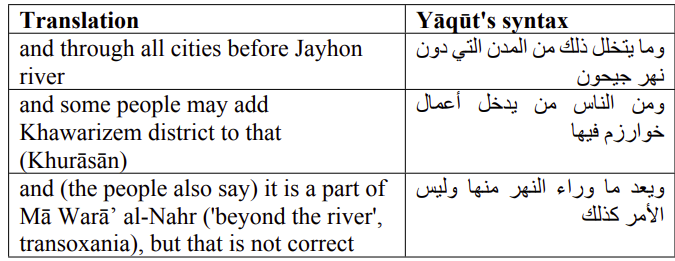
\includegraphics[width=0.7\linewidth]{figures/yaqut-with-translation} % Include the image with desired width
    \caption{Original, Arabic entries from Kitāb Mu'jam al-Buldān with their corresponding English tranlations~\cite{YaqutRB}} % Add a caption
    \label{fig:yaqut-entries} % Assign a label for referencing the figure in text
\end{figure}.

\subsection{Parsed Dataset - Places}
The layout of the gazetteer is highly structured, therefore, researchers were able to create a rule based method to parse
and expose the data in a tabular database~\cite{YaqutRB}.
This database provides serves as the primary datasource for this thesis.

\begin{figure}[h] % [h] attempts to place figure here, other options like [t]op, [b]ottom
    \centering % Centers the figure horizontally
    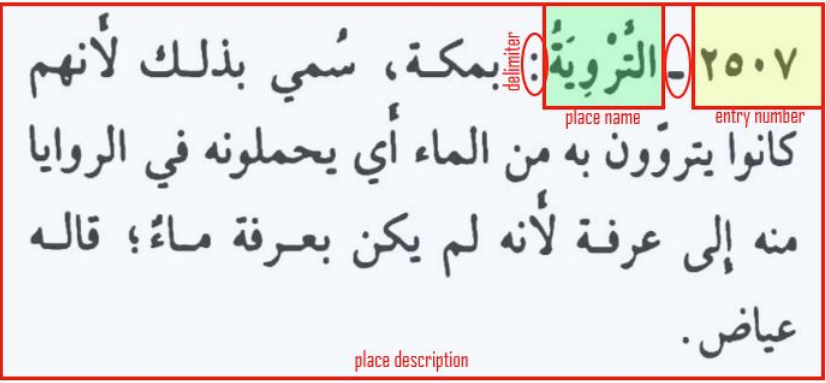
\includegraphics[width=0.8\linewidth]{figures/yaqut-layout} % Include the image with desired width
    \caption{Example of Muʿjam al-Buldān entry ~\cite{YaqutRB}} % Add a caption
    \label{fig:yaqut-structure} % Assign a label for referencing the figure in text
\end{figure}.

The primary, parsed datasource provided the following information:
\begin{itemize}
    \item Latitude
    \item Longitude
    \item Wikidata ID
    \item al-Turayyā ID~\cite{AlTurayya}
    \item Name (Arabic)
    \item Name (English)
    \item Type (lower hierarchy)
    \item Type (upper hierarchy)
    \item Metropolitan ID (reference to another place in the dataset)
    \item District ID (reference to another place in the dataset)
    \item Provincial ID (reference to another place in the dataset)
\end{itemize}


The only fields guaranteed to have data were the Arabic name and the unique identifier assigned based on the corresponding al-Turayyā gazetteer~\cite{AlTurayya}.

\subsubsection{al-Turayyā ID}
The IDs correspond to the database entries partially backing the al-Turayyā gazetteer project.
Namely, al-Turayyā used the same IDs to identify the OCR scanned entries.
A small caveat is that~\cite{YaqutRB} occasionally parsed multiple place descriptions from the same entry,
therefore, these entries have additional suffixes after the al-Turayyā ID to keep them unique.

\subsubsection{Wikidata ID}
Some more well known and easily identifiable place entries such as Baghdad were already enriched with Wikidata~\cite{Wikidata} IDs.
This information was initially used to build some graphs, but later iterations forewent its use due to the unreliability.
As an example, the entry for Mecca, which is a highly central and important node had the Wikidata ID of Q3289054
which refers to a city in the United States, not to the Saudi Arabian city.

\subsubsection{Categories}
The rule based parsing system also attempts to assign a category to each place entry.
The categories are selected from a pre-defined hand verified list.

The categories are split into a two level hierarchy.
For example, the level one category "town" has multiple sub-categories, like
village, small town, neighboring villages or abodes.

However, not all entries necessarily will have a secondary category.
In total there are 96 distinct categories.

\subsection{Parsed Dataset - Distances}
The other important block of data available in the parsed dataset are the distances.
There are over a thousand entries parsed from the original book, that express some spatial relationship
between two places.

The dataset this thesis works with, already contains this information in kilometres, but it is important
to keep in mind that the kilometer values provided are highly varying in terms of accuracy. This
is due to the fact that the original entries defined distance in terms of various non-standard methods
such as days of walking, travelling on camel back and so on.




\section{Relevant Concepts and Technologies}\label{sec:relevant-concepts}

\subsection{Knowledge Graphs}\label{subsec:introduction-knowledge-graphs}

\begin{wrapfigure}{r}{0.5\textwidth} % Float right, width half the text width
    \centering
    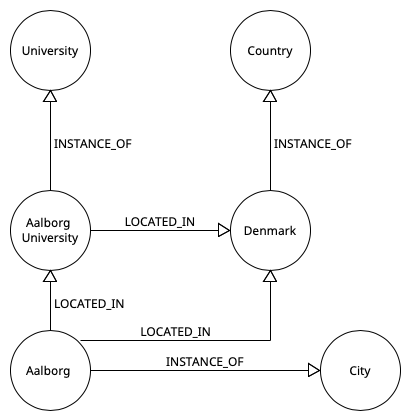
\includegraphics[width=\linewidth, scale=0.5]{figures/kg-example}
    \caption{Example of a knowledge graph.}
    \label{fig:kg-example}
\end{wrapfigure}
While there is no formal, widely accepted definition of Knowledge Graphs, one may think of them as a directed heterogeneous graphs
created with the intent of representing knowledge bases in a machine interpretable manner.

Nodes may (but not bound to) be objects, events, situations, abstract concepts or locations,
with the edges between the nodes representing conceptual relationships among the entities.

Knowledge graphs are often represented as lists of statements such that a statement is: $s = (h,r,t)$
where $h$ refers to the head entity, $t$ represents the tail entity and $r$ represents the
edge connecting the two entities.
These statements have also been called triplets.


Knowledge graphs are often backed by predefined ontologies.
Ontologies define entities and relationships referenced in the list of statements.
serving as their explicit schema, making the parsing of and
work with these graphs easier.

One may also think of knowledge graphs as the combination of the statements, and the relevant ontologies.

Some use cases of knowledge graphs include Google's enhanced contextual response to search queries~\cite{GoogleKnowledgeGraph} (using their internal
knowledge graph) or a more recent example: researchers have been experimenting with augmenting large language models
with knowledge graphs~\cite{LLMKG}, in order to ensure factual answers.

Examples of publicly available knowledge graphs are: Wikidata~\cite{Wikidata} a generic
knowledge graph backing the rest of the Wikimedia ecosystem, or WN18 dataset parsed from WordNet
introduced by~\cite{TransE} and is commonly used to evaluate the performance of various graph machine learning models.



\FloatBarrier
\subsection{Graph Representation Learning}\label{subsec:introduction-graph-representation-learning}
Graph Representation Learning is a research field dedicated to create various methods of embedding nodes of a graph into
a low dimensional vector space that may be used to perform various downstream tasks such as graph and node classification, or link prediction.

These GRL models rely on an encoder-decoder model.
"The intuition behind the encoder-decoder idea is the following:
if we can learn to decode high-dimensional graph information—such as the global positions of
nodes in the graph or the structure of local graph neighborhoods—from encoded low-dimensional embeddings, then, in principle,
these embeddings should contain all information necessary for downstream machine learning tasks"~\cite{RLGMandA}

In other words, while downstream tasks consume the vector representation, the decoder is used to create a well-trained encoder model.

The encoder may create either shallow embeddings, or deep embeddings.
Shallow embedding techniques are generally simpler and faster to train, but
may struggle to capture highly complex patterns and hierarchical relationships within the graph.

Example of shallow embedding methods include: Node2Vec~\cite{Node2vec} or DeepWalk~\cite{DeepWalk}

Deep embedding methods are commonly some variation of Graph Neural Networks detailed in section~\ref{subsec:introduction-graph-neural-networks}

\subsection{Graph Neural Networks}\label{subsec:introduction-graph-neural-networks}
The challenge in creating encoding models that capture deep insight into graph structures, is that graph structures are inherently variable ~\cite{GRLBook}.

For example, if one was to build a model that categorizes social networks using classical tools such as Convolutional Neural Networks or Recurring Neural Networks,
the model would be restricted to graphs with a set amount of nodes.

To address the above issue, and the leverage the structure of graphs Graph Neural Networks are used, which leverage the concept of Neural Message Passing.
The recent state-of-the art knowledge graph completion models are commonly based on some neural message passing framework~\cite{LPSOTA}, due to their inherent ability to capture
deeper neighborhood structures.

\begin{figure}[h] % [h] attempts to place figure here, other options like [t]op, [b]ottom
    \centering % Centers the figure horizontally
    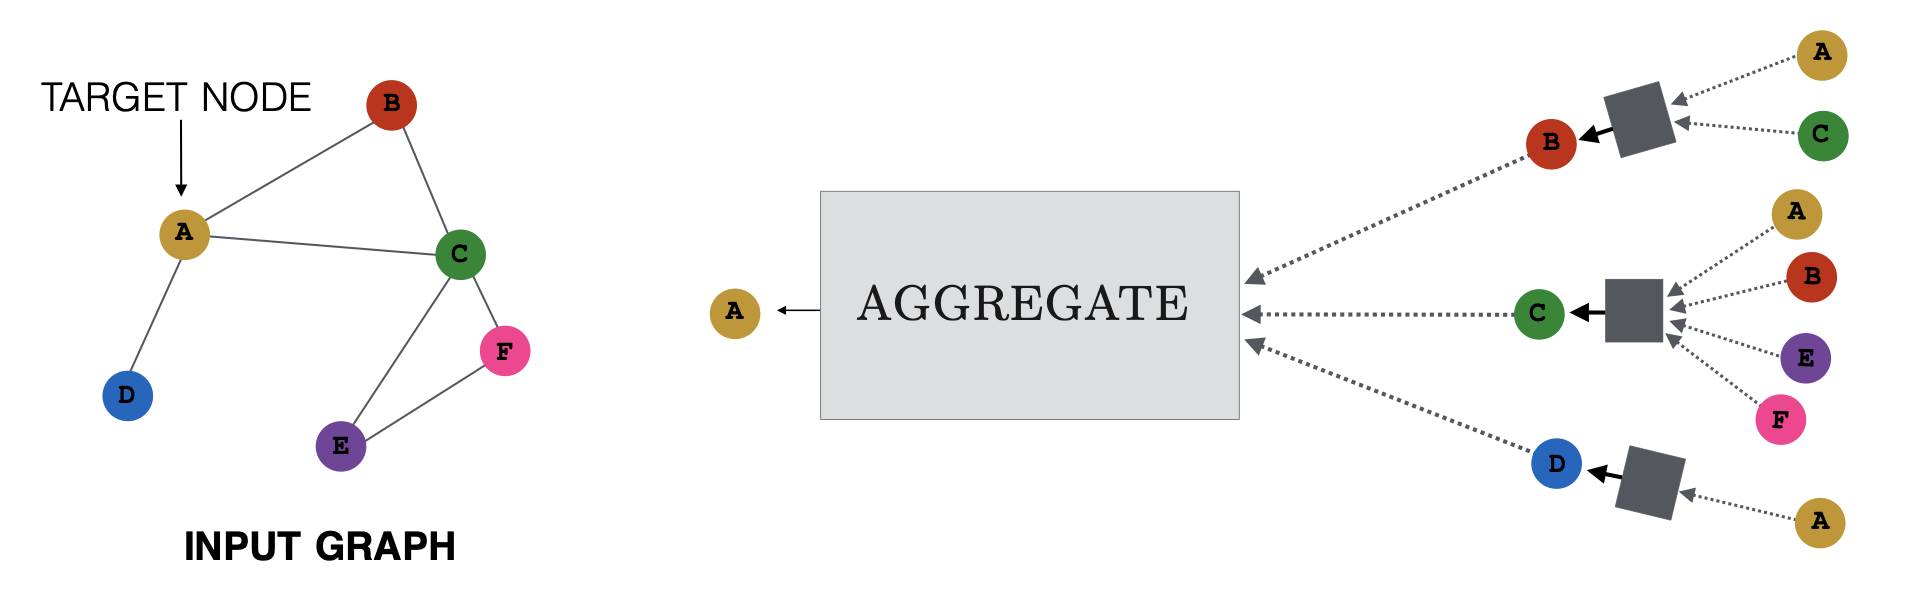
\includegraphics[width=0.9\linewidth]{figures/gnn} % Include the image with desired width
    \caption{A figure from the book, Graph Representation Learning~\cite{GRLBook} showcasing the general intuition behind neural message passing.} % Add a caption
    \label{fig:gnn} % Assign a label for referencing the figure in text
\end{figure}


\subsection{Wikidata}\label{subsec:introduction-wikidata}
"Wikidata is a free, collaborative, multilingual, secondary knowledge base, collecting structured data to provide support for Wikipedia, Wikimedia Commons, the other wikis of the Wikimedia movement,
and to anyone in the world."

"The Wikidata repository consists mainly of items, each one having a label, a description and any number of aliases.
Items are uniquely identified by a Q followed by a number, such as Douglas Adams (Q42).
Statements describe detailed characteristics of an Item and consist of a property and a value.
Properties in Wikidata have a P followed by a number, such as with educated at (P69)."~\cite{Wikidata}

As detailed later in section~\ref{sec:graph-building} the initial dataset that forms the basis of this thesis contains a number of nodes that have inferred Wikidata Ids.
Therefore, Wikidata will be used as a potential source for enriching the dataset, creating a denser network.

Moreover, a secondary object of this thesis is to represent Kitāb Mu'jam al-Buldān in a consumable knowledge graph format.
Therefore, it is easy to argue that using Wikidata's ontology will streamline such efforts.

\subsection{Neo4j}\label{subsec:introduction-neo4j}
During the development stages of this thesis, a heavily used tool was Neo4J~\cite{Neo4j}.
Neo4J is a No-SQL database engine, designed to store and manipulate graph-like structures.
The end user may access and modify the data via Neo4J's custom query language - Cypher.

While other similar graph database engines are available and would have been sufficient, this project uses Neo4J
due to its wide adoption and subsequent easy of access to relevant information.



\chapter{Building the Initial Graph and its Analysis}\label{ch:graph-analisys}

\section{Building the Graph}\label{sec:graph-building}
Within this thesis, there are two target edge categories that are valuable to predict: distance, and hierarchy.
Therefore, it is reasonable to create an initial investigative graph containing this information.

The graph will contain only place nodes, one node for each unique place ID. For simplicity, the distance edges
will not yet be binned, and each hierarchical relationship will explicitly be defined instead of relying on meta-paths.

The database engine storing the graph will be Neo4J, populated by a Python script while the analysis will be mainly done
with Gephi~\cite{Gephi}.

While building the graph, it became apparent that the number of disconnected nodes are exceedingly high (6289 nodes are orphans out of 14863 total nodes), therefore
the decision was made to only consider connected nodes as part of the graph, especially since the link prediction methods
require at least some connections.

\section{Initial Analysis}\label{sec:initial-analysis}
\subsection{Network Density and Connectivity}\label{subsec:network-density-and-connectivity}


Even with the disconnected nodes removed, the graph appears to be extremely sparse.
This is apparent from the density, which  may be calculated as follows:
\[
    D = \frac{2E}{N(N - 1)}
\]

With 8574 nodes and 10790 edges, the density is $~0.00029$.
Considering that a graph's density such that: ($0 \leq density \leq 1$), this graph is rather disconnected.

\subsection{Average Degree and Degree Distribution}\label{subsec:average-degree-and-degree-distribution}
The average degree of a node is 1.258, which again reinforces the perception of a sparse graph.
This low density may cause problems down the line, as link prediction methods commonly perform better on denser graphs.

The degree distribution (figure~\ref{fig:degree-distribution})
shows that there are a few nodes in the graph that are exceedingly central
(upwards of 6000 edges).
After some investigation,
it was found that these nodes generally correspond to large medieval cities or countries such as Baghdad,
Alexandria or Yemen.

Besides these highly central nodes, the degree distribution is fairly spread out.

\begin{figure}[h] % [h] attempts to place figure here, other options like [t]op, [b]ottom
    \centering % Centers the figure horizontally
    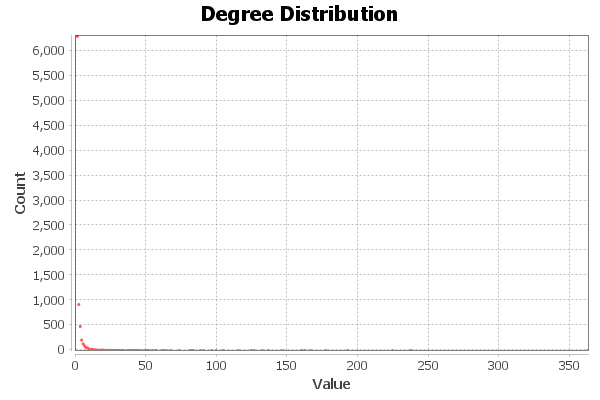
\includegraphics[width=1\linewidth]{figures/degree-distribution/degree-distribution} % Include the image with desired width
    \caption{Degree Distribution of the Initial Graph} % Add a caption
    \label{fig:degree-distribution} % Assign a label for referencing the figure in text
\end{figure}


\subsection{Modularity}\label{subsec:modularity}
Using Gephi's~\cite{Gephi} implementation of the Louvian method~\cite{Louvian} with a resolution of 5.0,
217 communities were found.

However, the high number of communities is only indicative of a highly disconnected graph, with many small, isolated node islands.
In practice there are 8 large groups accounting for 94.62\% of the nodes.

The modularity breakdown is shown on table:~\ref{tab:luv-communities}


\begin{table}[]
\centering
\begin{tabular}{|l|l|l|}
\hline
\textbf{Name} & \textbf{Population} & \textbf{Color on Figure ~\ref{fig:communities}} \\ \hline
Group 1       & 22.26\%             & Pink                     \\ \hline
Group 2       & 17.46\%             & Green                    \\ \hline
Group 3       & 15.13\%             & Blue                     \\ \hline
Group 4       & 9.41\%              & Black                    \\ \hline
Group 5       & 9\%                 & Orange                   \\ \hline
Group 6       & 8.69\%              & Red                      \\ \hline
Group 7       & 6.85\%                & Yellow                   \\ \hline
Group 8       & 5.82\%                & Cyan                     \\ \hline
\end{tabular}
\caption{Communities ratios detected by the Louvain method}
\label{tab:luv-communities}
\end{table}

Figure~\ref{fig:communities} shows that the detected, large communities are fairly easy to visually distinguish.
Moreover, it shows that the highly central nodes (visualized via larger diameter) are spread around the communities fairly evenly.

\begin{figure}[h] % [h] attempts to place figure here, other options like [t]op, [b]ottom
    \centering % Centers the figure horizontally
    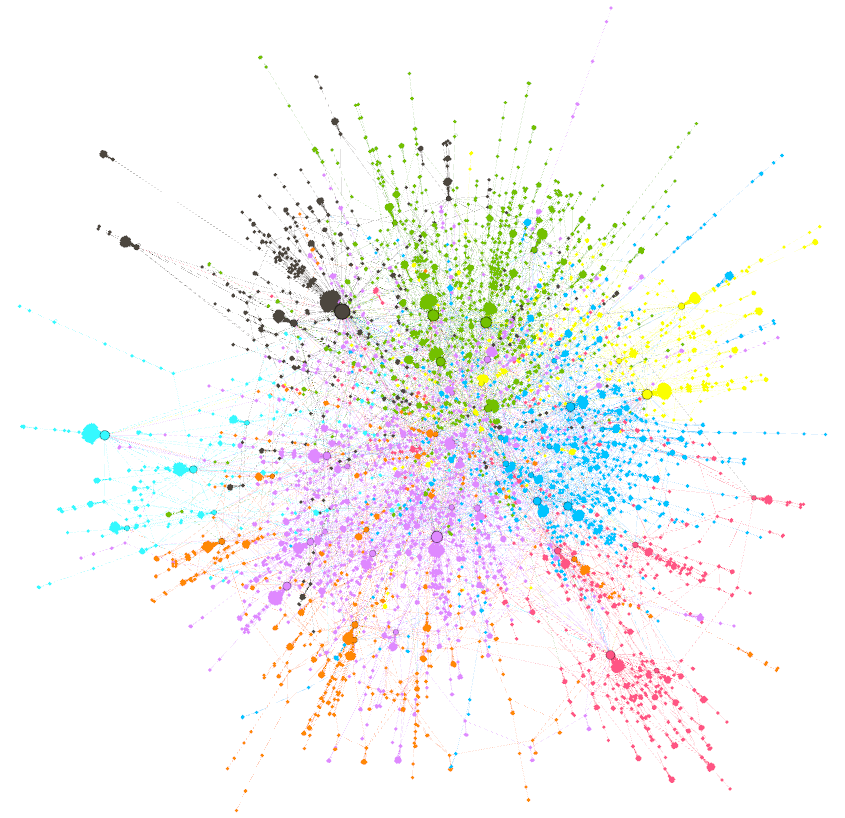
\includegraphics[width=0.7\linewidth]{figures/modules} % Include the image with desired width
    \caption{Graph visualization showing the communities listed on table~\ref{tab:luv-communities}} % Add a caption
    \label{fig:communities} % Assign a label for referencing the figure in text
\end{figure}.


\subsection{Unexpected Patterns}\label{subsec:odd-patterns}

While working with the parsed dataset, some odd patterns were found.
First, \textbf{DISTANCE} triplets were found, where both the head and tail entity were the same.
At the recommendation of the authors of ~\cite{YaqutRB} these triplets were discarded.



\begin{figure}[h] % [h] attempts to place figure here, other options like [t]op, [b]ottom
    \centering % Centers the figure horizontally
    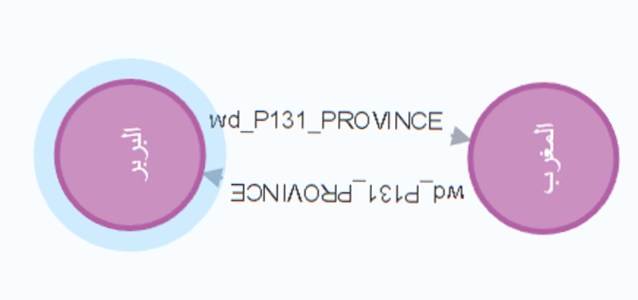
\includegraphics[width=0.5\linewidth]{figures/odd1} % Include the image with desired width
    \caption{Unusual hierarchical pattern where two nodes reference each other as their province.} % Add a caption
    \label{fig:odd1} % Assign a label for referencing the figure in text
\end{figure}

Secondly, during manual observation of the data, "odd" hierarchical patterns were observed;
that did not fit to the classical strict, unidirectional layout of other similar structures, shown on figure~\ref{fig:odd1} and ~\ref{fig:odd2} .

\begin{figure}[h] % [h] attempts to place figure here, other options like [t]op, [b]ottom
    \centering % Centers the figure horizontally
    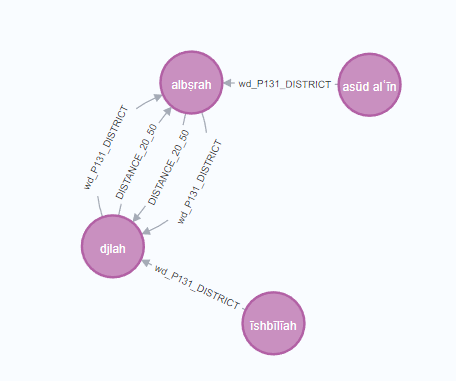
\includegraphics[width=0.5\linewidth]{figures/odd2} % Include the image with desired width
    \caption{Unusual hierarchical pattern where two nodes reference each other as their district.} % Add a caption
    \label{fig:odd2} % Assign a label for referencing the figure in text
\end{figure}

These patterns were extracted and forwarded to the Mehdie researchers using the following Neo4J query:
\begin{verbatim}
    MATCH (n)-[:{r1}]->(m)-[:{r2}]->(n) RETURN n,m
\end{verbatim}

Where r1 and r2 correspond to all potential pairwise combinations of the edge types:
\textbf{wd\_P131\_METROPOLITAN}, \textbf{wd\_P131\_DISTRICT} and \textbf{wd\_P131\_PROVINCE}


\chapter{Knowledge Graph Embedding Methods}\label{ch:knowledge-graph-embedding-methods}
The first broad classification of link prediction methods explored in this thesis are the knowledge graph embedding methods (KGE).
Since graph neural networks generate node embeddings as well, the terminology is somewhat ambiguous.
The following few paragraphs will attempt to clearly distinguish the class of methods detailed in this chapter.

KGE methods attempt to position each node in a vector space (figure~\ref{fig:vec-space-vis}).
In a well-trained model, nodes from the same neighborhood will be placed near each other within the vector space.
Moreover, these positions are strictly unique, i.e.\ two distinct nodes cannot occupy the same place.
From this, naturally follows that KGE methods are strictly transductive, and cannot generalize.

Fortunately, a transductive setting is not necessarily limiting for the purposes of this thesis.
(TODO: WorldKG), as all the link-predictions tasks are limited
to the domain of places mentioned in Kitāb Mu'jam al-Buldān.

While there are exceptions to this rule, such as the ComplEx~\cite{ComplEx} discussed in TODO: ComplexRef
KGE methods are generally more efficient and easily more scalable than their GNN counterparts.
\begin{figure}[h] % [h] attempts to place figure here, other options like [t]op, [b]ottom
    \centering % Centers the figure horizontally
    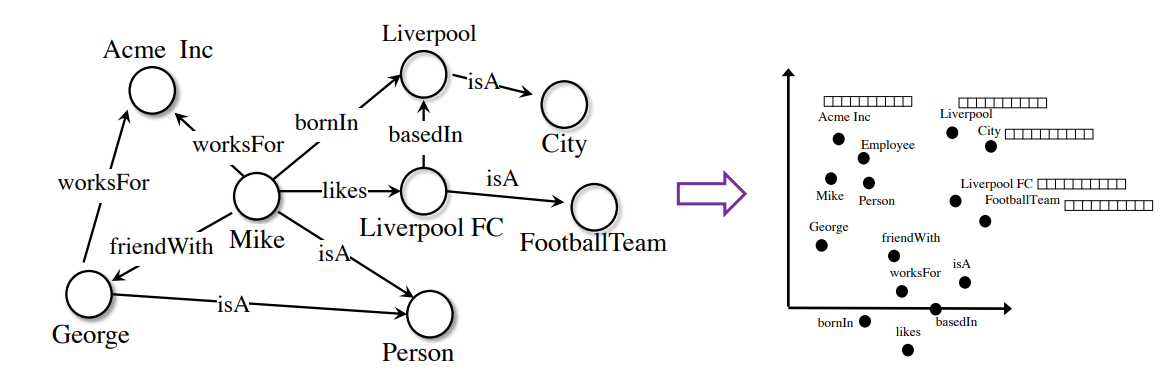
\includegraphics[width=1\linewidth]{figures/vector-space} % Include the image with desired width
    \caption{Visualization of Vector Space Embedding~\cite{KGETutorial}} % Add a caption
    \label{fig:vec-space-vis} % Assign a label for referencing the figure in text
\end{figure}.
\section{General Architecture}
Generally, KGE models, at least within the context of this thesis, fit into the same generic architecture (figure~\ref{fig:kge-architecture}).

\begin{figure}[h] % [h] attempts to place figure here, other options like [t]op, [b]ottom
    \centering % Centers the figure horizontally
    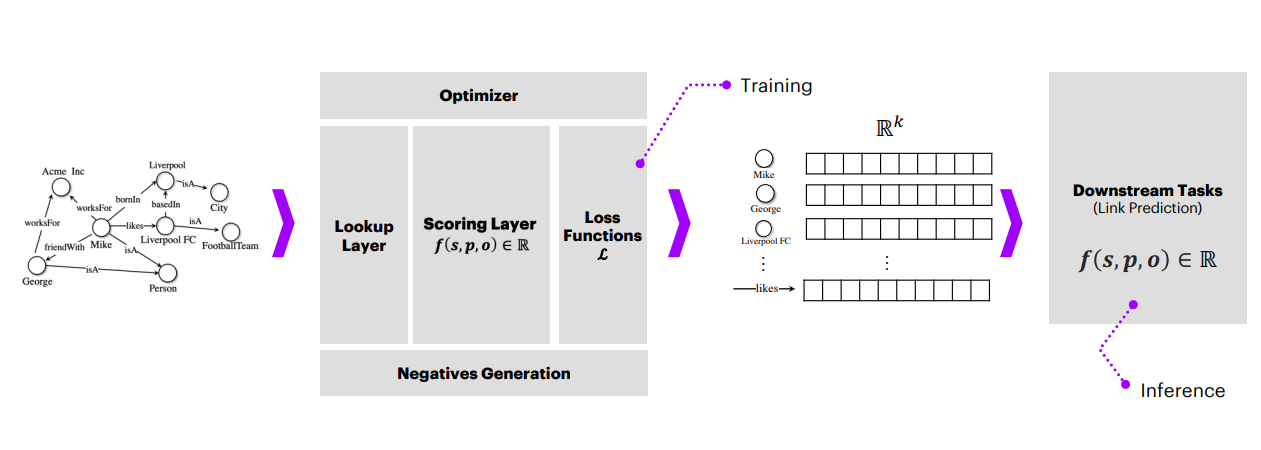
\includegraphics[width=1\linewidth]{figures/kge-architecture} % Include the image with desired width
    \caption{Generic KGE architecture~\cite{KGETutorial}} % Add a caption
    \label{fig:kge-architecture} % Assign a label for referencing the figure in text
\end{figure}.

\subsection{Lookup Layer}
The Lookup layer just simply functions as a dictionary between the individual nodes and relationships and their respective embeddings.
\subsection{Scoring Layer}
Colloquially, the heart of the architecture, the scoring layer takes the encoding of each member of the triplet
and assigns a score to the whole statement.
The higher the score, the more likely it is that the statement is a true statement.
The specific scoring functions are detailed in section~\ref{sec:embedding-methods}

\subsection{Loss Function}
As with all other neural models; the generic KGE architecture relies on a loss function, which is necessary to optimize the model.
In the KGE section of this thesis, two loss functions were used.

\subsubsection{Pairwise, Max-margin Loss}
This function penalizes the model if the score assigned by scoring function $f_{model}$
to a positive triple $t^+$ selected from the set of positives $\mathcal{G}$, is lower than the score assigned to a
negative triple $t^-$ selected from the set of corruptions $\mathcal{C}$
by margin $\gamma$

\begin{gather*}
    \mathcal{L}(\Theta) = \sum_{t^+ \in \mathcal{G}}\sum_{t^- \in \mathcal{C}}max(0, [\gamma + f_{model}(t^-;\Theta)
 - f_{model}(t^+;\Theta)])
\end{gather*}

\subsubsection{Negative Log-Likelihood Loss}
Another commonly used loss function, $y \in -1,1 $ dependent on whether the statement is positive or negative.
\begin{gather*}
    \mathcal{L}(\Theta) = \sum_{t \in \mathcal{G} \cup \mathcal{C}}log(1 + exp(-y \, f_{model}(t;\Theta)))
\end{gather*}

\subsection{Negatives Generation}\label{subsec:negatives-generation}
A very distinctive feature of the domain of knowledge graph link prediction is the (usual) lack of true negative data points.
Let's consider the domain of image recognition.
If someone were to train a model to detect the presence of a cat in a photo,
the negative data points could be any photos that do not contain a cat.
However, in the case of knowledge graphs, there are no negative facts.
A knowledge graph may contain the triplet \textit{<London,CapitalOf,UnitedKingdom>}

And even though for a human reader, this automatically means that \textit{<London, CapitalOf, Denmark>} is a false statement,
a normal knowledge graph will not contain such information explicitly.
Therefore, link prediction methods commonly rely on some form of synthetic negative triplet generation.

While there have been many strategies proposed~\cite{NegSamp}, in this thesis, a very simple method was chosen.
Given a true statement $s = (h,r,t)$, a negative sample will be generated by corrupting $t$ by randomly replacing it with another node from the graph.
Of course, corruption is done with consideration of the ground truth triplets.

This has a negative effect under the open world assumption
of potentially labeling unknown true positives as negative data points ~\cite{OpenWorld}.
However, due to its simplicity, this approach has the benefit of avoiding any potential bias in the training
and being computationally efficient.

\subsection{Optimizer}
Same concept as in other machine learning architectures, in this thesis two optimizers were used:
Adam~\cite{Adam} and AdaGrad~\cite{Adagrad}


\section{Embedding Methods}\label{sec:embedding-methods}
\subsection{Translating Embeddings (TransE)}
Commonly used benchmark, and one of the first KGE models.
This approach attempts to model relationships as translations between two points (nodes) in a vector space

Given a statement $s = (h,r,t)$, ideally $h$ and $t$ should be close to each other in the vector space,
with the difference being the translation of the relation $r$~\cite{TransE}.


\begin{figure}[h] % [h] attempts to place figure here, other options like [t]op, [b]ottom
    \centering % Centers the figure horizontally
    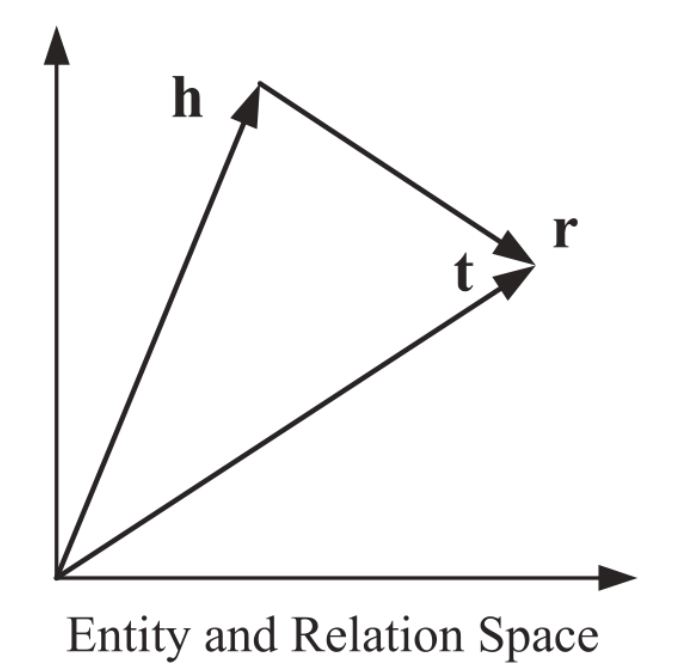
\includegraphics[width=0.35\linewidth]{figures/transe} % Include the image with desired width
    \caption{Visualization of TransE~\cite{TransEFig}}
    \label{fig:transe-example}
\end{figure}.

\FloatBarrier

\subsection{Relational Rotation Embeddings (RotatE)}
"The RotatE model maps
the entities and relations to the vector space and defines each relation as a rotation from
the source entity to the target entity."~\cite{RotatE}

The benefit of RotatE over TransE lies in expressiveness.
It is able to model more relationship patterns, such as symmetry, antisymmetry, inversion
and composition.

\begin{figure}[h] % [h] attempts to place figure here, other options like [t]op, [b]ottom
    \centering % Centers the figure horizontally
    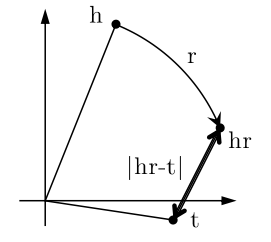
\includegraphics[width=0.35\linewidth]{figures/rotate} % Include the image with desired width
    \caption{Visualization of RotatE~\cite{RotatE}}
    \label{fig:rotate}
\end{figure}.

\FloatBarrier


\subsection{Holographic Embeddings (HolE)}

Holographic Embedding~\cite{HolE} is a model for learning representations of entities and relationships in a knowledge graph.
It uses the principles of holography and circular correlation to combine entity embeddings in a way that captures rich
interactions between entities and relations.

The main benefit of HolE over other approaches is the increased modeling power.

\subsection{The Bilinear Diagonal DistMult Model (DistMult)}

DistMult is a tensor factorization based model introduced in~\cite{DistMult} that uses,
trilinear dot product as its scoring function.

However, a big limitation of DistMult is that it cannot model asymmetric relationships.

\subsection{Complex Embeddings (ComplEx)}

ComplEx~\cite{ComplEx} is similar to DistMult in using the dot product of two vectors to calculate the score.
However, it uses the Hermitian dot product, which is able to handle asymmetrical relationships.

Moreover, instead of using real-valued vectors, DistMult uses a complex vector space for both entities and relations.
Allowing to capture richer information about the graph at the cost of increased computational cost.

\subsection{Benchmark Comparison of KGE Methods}
Table~\ref{tab:kge-perf-comp} shows the performance of the above detailed KGE methods on the FB15k benchmark dataset.


\begin{table}[!ht]
    \centering

    \begin{tabular}{|l|l|l|l|}
        \hline
         & MRR            & Hits@1                       & Hits@10               \\ \hline
TransE   & 0.463          & 0.29                         & 0.75                  \\ \hline
RotatE   & 0.797          & \textbf{0.746}               & 0.884                 \\ \hline
HolE     & 0.524          & 0.4                          & 0.73                  \\ \hline
DistMult & \textbf{0.841} &                              & \textbf{0.914}        \\ \hline
ComplEx  & 0.84           & 0.692 &  0.75                                        \\ \hline
\end{tabular}
\caption{Performance of Discussed KGE Methods on the FB15k Benchmark Dataset. Datasources~\cite{paperswithcode2024fb15k, HolE}}
\label{tab:kge-perf-comp}
\end{table}

\section{Methodology}
In the initial KGE experiments, the dataset generated in TODO was used as data for the models.
The dataset was split into train, test and validation dataset in a $80\%$, $10\%$ and $10\%$ ratio.
The split was done in a transductive manner, such that there are no, previously unseen nodes in the test and validation
dataset.

To find the best performing model and the most optimal hyperparameters, a grid search was performed, with the MRR score
being the basis of comparison.

For each method detailed in section TODO, the following hyperparameters were tuned:
\begin{itemize}
    \item \textbf{Batch size:} 128, 256, 512, 1024, 2048
    \item \textbf{Epochs:} 5, 25, 50, 100, 200, 250
    \item \textbf{Eta:} 5, 10, 15 (\textit{eta specifies the number of corruptions to generate per each positive})
    \item \textbf{Vector embedding size:} 50, 100, 150, 200
    \item \textbf{Loss function:} pairwise, nll
    \item \textbf{Optimizer:} AdaGrad, adam
\end{itemize}

The best performing model and hyperparameter combinations are shown on table~\ref{tab:kge-params}.

\begin{table}[!ht]
    \centering
    \begin{tabular}{|l|l|l|l|l|l|}
        \hline
        & \textbf{TransE} & \textbf{RotatE} & \textbf{HolE} & \textbf{DistMult} & \textbf{ComplEx} \\ \hline
        \textbf{Batch size} & 2048 & 1024 & 128 & 128 & 128 \\ \hline
        \textbf{Epochs} & 200 & 90 & 80 & 60 & 50 \\ \hline
        \textbf{k} & 150 & 150 & 200 & 200 & 200 \\ \hline
        \textbf{eta} & 5 & 15 & 5 & 5 & 5 \\ \hline
        \textbf{loss} & pairwise & nll & pairwise & pairwise & pairwise \\ \hline
        \textbf{optimizer} & adam & adam & adam & adam & adam \\ \hline
    \end{tabular}
    \caption{Best performing KGE hyperparameters}
    \label{tab:kge-params}
\end{table}
\section{Results}
Unfortunately, even with the tuned hyperparameters, the KGE models produced subpar results (table~\ref{tab:kge-res}).
With the highest MRR being $0.18$ produced by HolE, DistMult and ComplEx with DistMult slightly under-performing in
hits@10 compared to the other two.
\begin{table}[!ht]
    \centering
    \begin{tabular}{|l|l|l|l|l|}
        \hline
         & MRR & Hits@10 &  Hits@5 &  Hits@1 \\ \hline
        TransE & 0.11   & 0.24 & 0.14 & 0.04 \\ \hline
        RotatE & 0.16   & 0.21 & 0.17 & 0.13 \\ \hline
        HolE & 0.18     &  0.22 & 0.19 & 0.16 \\ \hline
        DistMult & 0.18 & 0.21 & 0.18 & 0.16 \\ \hline
        ComplEx & 0.18  & 0.22 & 0.19 & 0.16 \\ \hline
    \end{tabular}
    \caption{Performance of the hyperparameter tuned KGE models on a previously unseen test dataset}
    \label{tab:kge-res}
\end{table}

After some investigation, two apparent issues were found.
First, the kilometer values of distance edges range from ~1 kilometer to over 1000 kilometers.
Therefore, all the distance edges were binned into ranges.

Second, the model was incorrectly predicting not explicitly defined hierarchical information.
Since this information was available in the source dataset, it made sense to modify the training data
to include all available hierarchical information instead of expecting the model to learn the hierarchical meta-paths.

Finally, reverse edge types were introduced to increase the graph density.
These edges were only inserted after the train / test / validation split to avoid leakage.

The final edge composition in the data is shown on table~\ref{tab:kge-new-edges} (excluding the reverse edge counts
as they are obviously equal to their counterparts.).

\begin{table}[!ht]
    \centering
    \begin{tabular}{|l|l|}
        \hline
        \textbf{Edge Type } & \textbf{Count} \\ \hline
        DISTANCE\_0\_5 & 50 \\ \hline
        DISTANCE\_5\_10 & 48 \\ \hline
        DISTANCE\_10\_20 & 254 \\ \hline
        DISTANCE\_20\_50 & 690 \\ \hline
        DISTANCE\_50\_100 & 340 \\ \hline
        DISTANCE\_100\_200 & 294 \\ \hline
        DISTANCE\_200\_500 & 142 \\ \hline
        DISTANCE\_500\_1000 & 6 \\ \hline
        DISTANCE\_1000\_inf & 8 \\ \hline
        wd\_P17 & 3507 \\ \hline
        wd\_P31 & 13707 \\ \hline
        wd\_P131\_DISTRICT & 3124 \\ \hline
        wd\_P131\_METROPOLITAN & 4695 \\ \hline
        wd\_P131\_PROVINCE & 4252 \\ \hline
        wd\_P279 & 66 \\ \hline
        wd\_P206 & 223 \\ \hline
        wd\_P361 & 287 \\ \hline
        wd\_P706 & 57 \\ \hline
    \end{tabular}
    \caption{Edge Count of the Second Iteration of the KGE Experiments}
    \label{tab:kge-new-edges}
\end{table}

With the new training dataset, the hyperparameter tuning was repeated for each method.
Unfortunately it appears that the new dataset did not result in increased model performance.
In fact all across the board, the performance of the models decreased (table~\ref{tab:kge-new-res}).

However, it is important to point out that some of the reduction in performance may be attributed to the increased
difficulty in distance prediction.

\begin{table}[!ht]
    \centering
    \begin{tabular}{|l|l|l|l|l|}
        \hline
        & MRR & Hits@10 &  Hits@5 &  Hits@1 \\ \hline
        TransE & 0.09   & 0.24 & 0.12 & 0.037 \\ \hline
        RotatE & 0.07   & 0.14 & 0.09 & 0.039 \\ \hline
        HolE & 0.12     &  0.19 & 0.16 & 0.09 \\ \hline
        DistMult & 0.16 & 0.22 & 0.19 & 0.12 \\ \hline
        ComplEx & 0.16  & 0.22 & 0.2 & 0.13 \\ \hline
    \end{tabular}
    \caption{Performance of the hyperparameter tuned KGE models on a previously unseen test dataset}
    \label{tab:kge-new-res}
\end{table}

\chapter{Experiments with Neural Bellman-Ford Networks}\label{ch:nbfnet}


\section{Introduction}\label{sec:nbfnet-introduction}
After the lackluster result from the translation methods detailed in chapter~\ref{ch:knowledge-graph-embedding-methods}, the need for
experimentation with other approaches became apparent.

At the time of writing, the state-of-the art multi-relational link prediction methods~\cite{LPSOTA} are generally
based on, and expand on the message passing, Graph Neural network architecture.

Specifically, the top performing model, according to the Papers with Code benchmark on FB15k-237 link prediction~\cite{NBFNetSota}
are the Neural Bellman-Ford Networks (NBFNet).

Therefore, from now on, this thesis will focus on training an NBFNet model on the Kitāb Mu'jam al-Buldān dataset.


\section{Brief Overview of Neural Bellman-Ford Networks}\label{sec:nbfnet-description}
\subsection{Generalization of Graph Heuristics}\label{subsec:generalization-of-graph-heuristics}

The first intuition behind NBFNet is that many of the traditional graph heuristics such as Katz-Index, Personalized PageRank~\cite{Page1998PageRank}
or Graph Distance can be generalized into a \textit{multiplication} and a \textit{summation} step.

\begin{figure}[h] % [h] attempts to place figure here, other options like [t]op, [b]ottom
    \centering % Centers the figure horizontally
    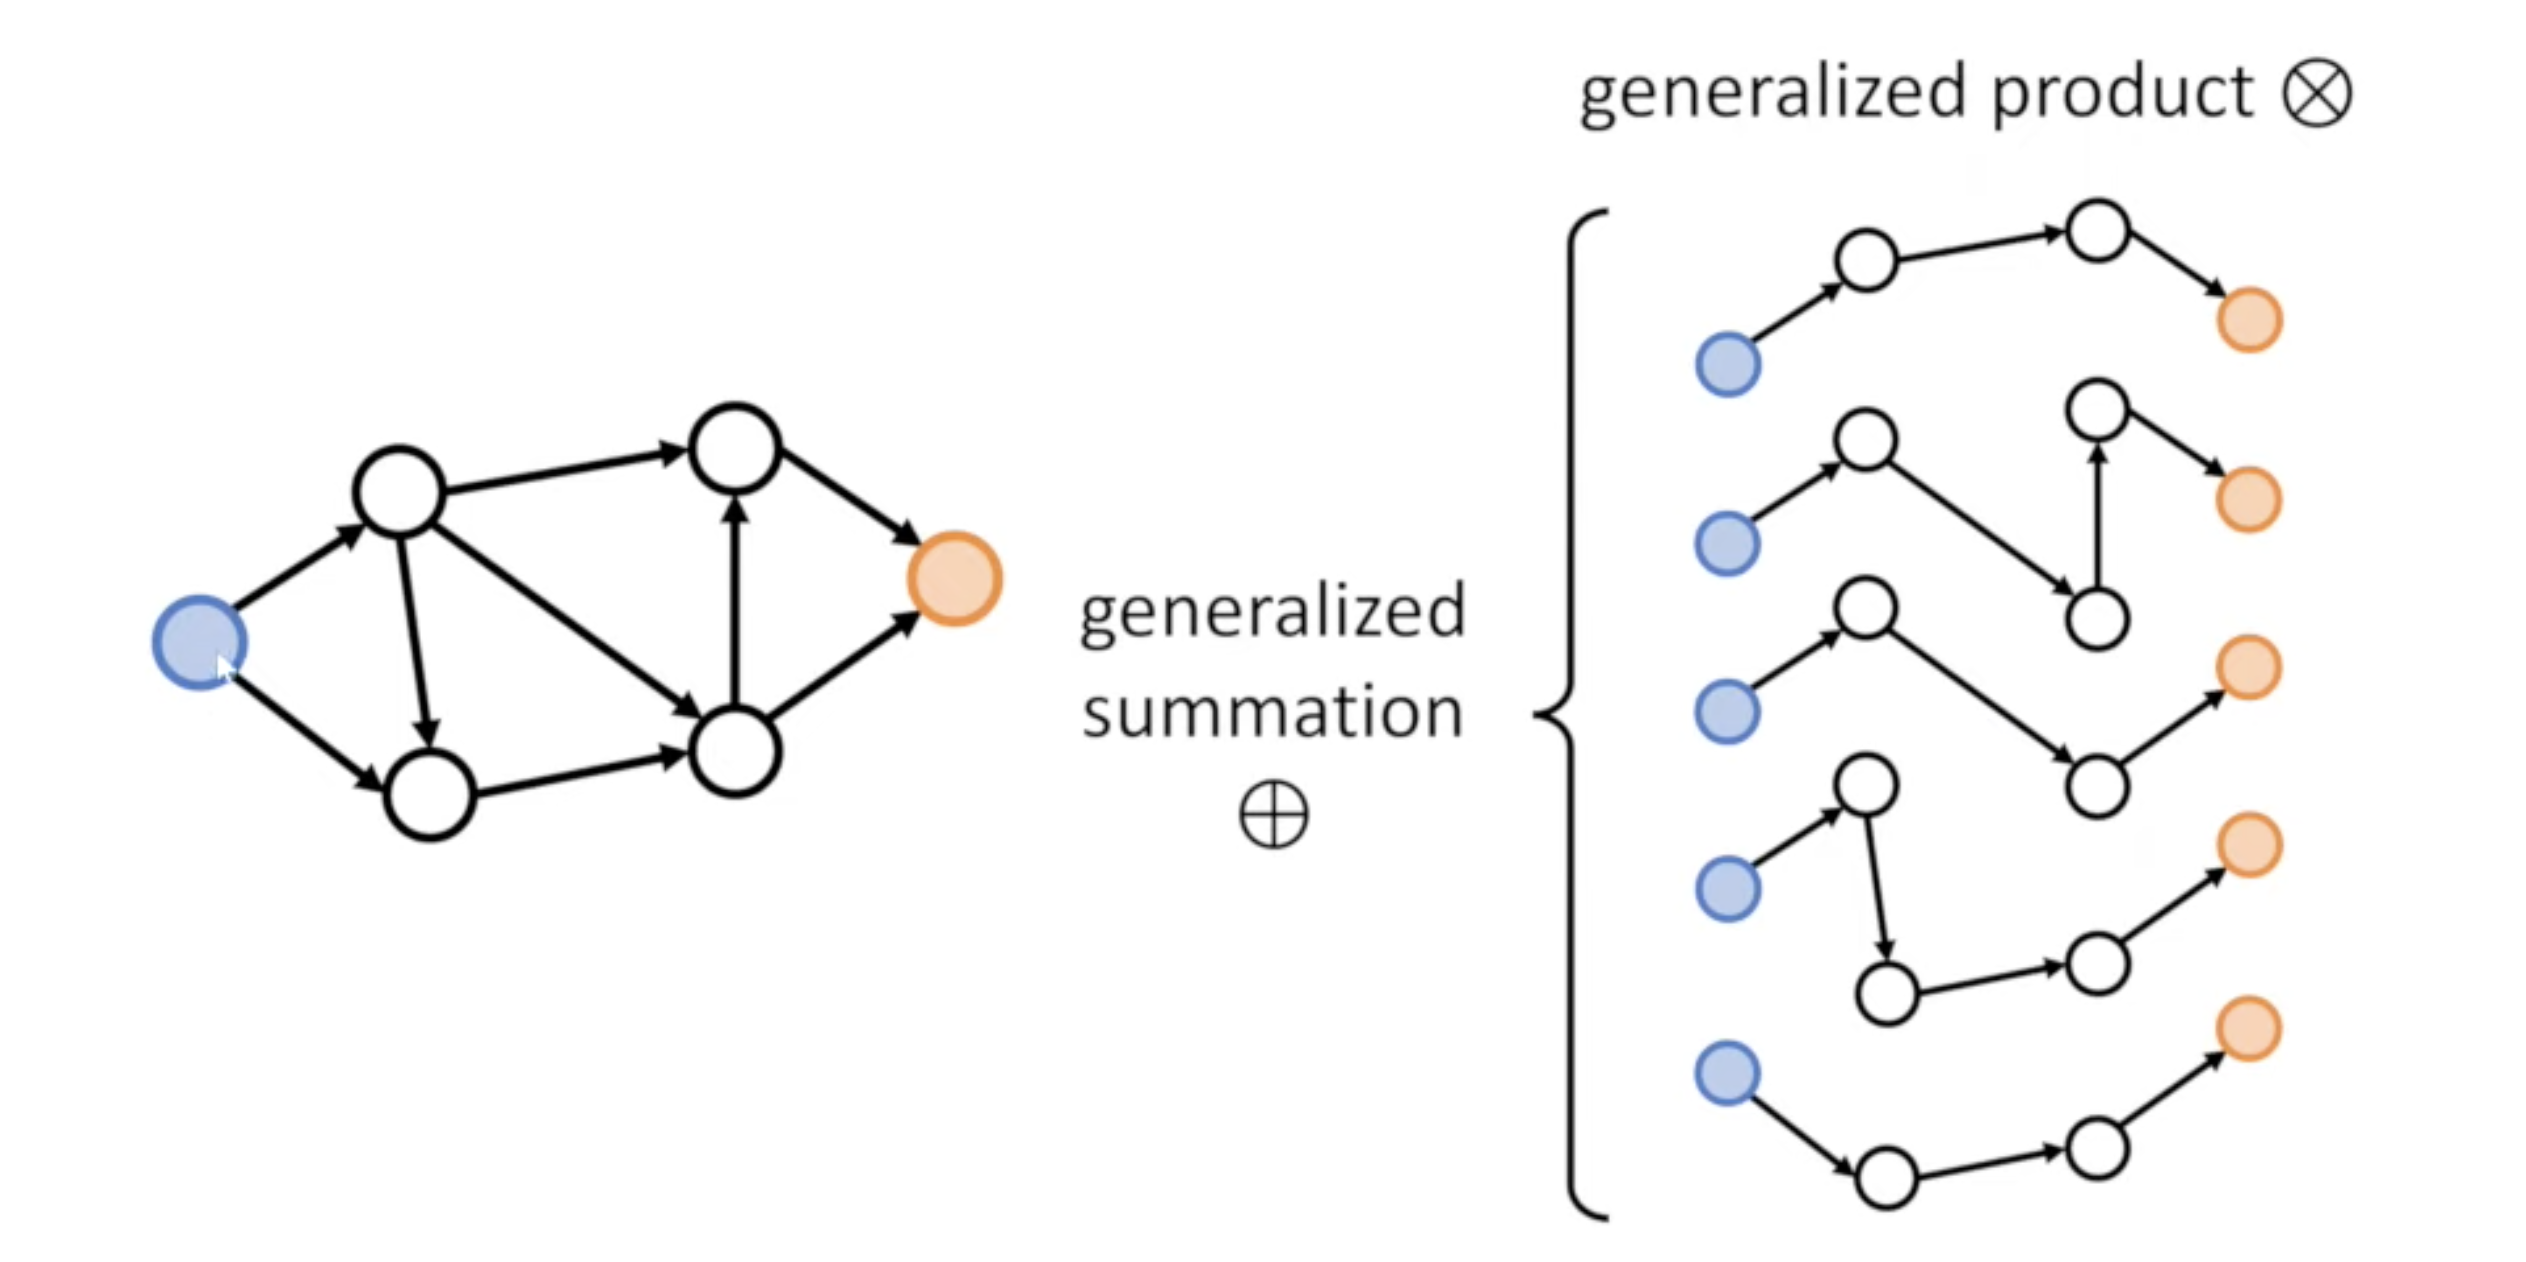
\includegraphics[width=0.8\linewidth]{figures/nbfnet-trad} % Include the image with desired width
    \caption{Generalized Graph Heuristic ~\cite{NBfnetPres}} % Add a caption
    \label{fig:nbfnet-trad} % Assign a label for referencing the figure in text
\end{figure}

For example, to find the shortest Graph Distance between two nodes, first we count the number of hops (generalized multiplication step by count) and then we select
the path with the fewest hop (generalized summation via the min function)

The second intuition behind NBFNet is that traditional link prediction methods that rely on encapsulating local neighborhoods~ ~\cite{RandomWalks, SubgraphExtraction}
perform random walks between the source and the target node.

Instead of these random walks, the pair representation can be formulated as "a generalized sum of path representations between u and v with a commutative
summation operator \bigoplus"~\cite{NBFNet}.

Within this summation, each path "is defined as a generalized product of the edge
representations in the path with the multiplication operator"~\cite{NBFNet}.

\subsection{Generalized Bellman-Ford Algorithm}\label{subsec:generalized-bellman-ford-algorithm}

Calculating such metrics for each node pair is computationally expensive due to its exponential nature.
As a solution, the NBFNet performs these calculations as part of a generalized Bellman-Ford algorithm, as that algorithm is highly
parallelizable (figure~\ref{fig:gen-bf}).

\begin{figure}[h] % [h] attempts to place figure here, other options like [t]op, [b]ottom
    \centering % Centers the figure horizontally
    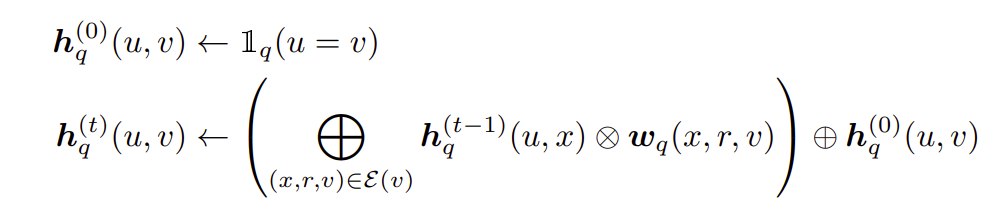
\includegraphics[width=0.8\linewidth]{figures/nbfnet-gen-bf} % Include the image with desired width
    \caption{Generalized Bellman-Ford Algorithm ~\cite{NBFNet}} % Add a caption
    \label{fig:gen-bf} % Assign a label for referencing the figure in text
\end{figure}

\subsection{Neural Bellman-Ford Networks}\label{subsec:neural-bellman-ford-networks}
Finally, to increase the potential of the models and detach from classical, handcrafted methods, the creators of NBFNet replaced
the generalized \textit{summation} and \textit{multiplication} operators with neural functions.

A Neural Bellman-Ford Network has three neural functions.

\subsubsection{The INDICATOR function}
"The INDICATOR function initializes a
representation on each node, which is
taken as the boundary condition of the generalized Bellman-Ford algorithm."~\cite{NBFNet}

It replaces the $\textbf{h}_q^{(0)}(u,v)\leftarrow\ \mathbbm{1}_q(u=v)$ step, seen on figure~\ref{fig:gen-bf}

\subsubsection{The MESSAGE function}
"The MESSAGE function replaces the binary multiplication operator \bigotimes"~\cite{NBFNet}


\subsubsection{The AGGREGATE function}
"The AGGREGATE function is a permutation invariant function
over sets that replaces the n-ary summation operator $\bigoplus$ \ldots
one may alternatively define AGGREGATE as the commutative binary operator $\bigoplus$ and apply it
to a sequence of messages." ~\cite{NBFNet}


The combination of the three neural function are shown on figure~\ref{fig:neural-bf}.

\begin{figure}[h] % [h] attempts to place figure here, other options like [t]op, [b]ottom
    \centering % Centers the figure horizontally
    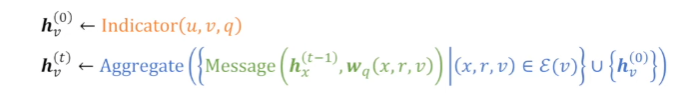
\includegraphics[width=0.65\linewidth]{figures/nbfnet-architecture} % Include the image with desired width
    \caption{Neural Bellman-Ford Network Architecture ~\cite{NBfnetPres}} % Add a caption
    \label{fig:neural-bf} % Assign a label for referencing the figure in text
\end{figure}


Finally, the learned vector representation is then fed into a multi-layer perceptron to predict the probability
of a tail node given a head node and a query relationship (figure~\ref{fig:nbfnet-mlp})

\begin{figure}[h] % [h] attempts to place figure here, other options like [t]op, [b]ottom
    \centering % Centers the figure horizontally
    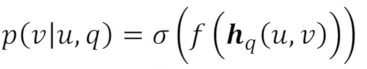
\includegraphics[width=0.4\linewidth]{figures/nbfnet-mlp} % Include the image with desired width
    \caption{Final Prediction Step in NBFNet ~\cite{NBfnetPres}} % Add a caption
    \label{fig:nbfnet-mlp} % Assign a label for referencing the figure in text
\end{figure}



\section{Methodology}\label{sec:nbfnet-methodology}
The training of the model was mainly done using the Pyg implementation of NBFNet, a codebase written by the original authors~\cite{NBFNet_PyG}.

PNA DIST mult

transductive 8-1-1 split

\section{Results}\label{sec:nbfnet-results}
Unfortunately,
the performance of the trained NBFNet model (table~\ref{tab:nbfnet-res})
on the previously unseen test dataset was comparable to
the performance of the initial KGE models.
It performed slightly worse in terms of MRR, but it achieved the highest score on Hits@10 and Hits@5

\begin{table}[!ht]
    \centering
    \begin{tabular}{|l|l|l|l|l|}
        \hline
        & MRR & Hits@10 & Hits@5 & Hits@1 \\ \hline
        TransE & 0.11   & 0.24 & 0.14 & 0.04 \\ \hline
        RotatE & 0.16   & 0.21 & 0.17 & 0.13 \\ \hline
        HolE & 0.18     &  0.22 & 0.19 & 0.16 \\ \hline
        DistMult & 0.18 & 0.21 & 0.18 & 0.16 \\ \hline
        ComplEx & 0.18  & 0.22 & 0.19 & 0.16 \\ \hline
        NBFNet & 0.17 & \textbf{0.27} & \textbf{0.21} & 0.11 \\ \hline
    \end{tabular}
    \caption{Performance of the KGE and NBFNet models}
    \label{tab:nbfnet-res}
\end{table}

A potential approach to improve the model's performance is discussed in the next chapter.
\chapter{Pretrained WorldKG NBFNet Model}\label{ch:worldkg}
The previous experiments in chapter TODO and chapter TODO show that regardless of the class of approach used,
there is a fundamental barrier when working with this thesis' knowledge graph.
Namely, there is a high chance that the sparsity of the graph prevents
any potential model from properly being able to generalize.

As a solution, this thesis proposes an alternate approach.
Instead of trying additional models, the previously used
NBFNet model could be pre-trained on a denser graph.
Since the Kitāb KG, ultimately is just the graph representation of a geospatial area,
it is relatively easy to create a synthetic dataset that mimics it.
Moreover, creating such a dataset allows for the introduction of specific distance edge biases, not generally present in Kitāb, that could provide valuable information to researchers.
Pre-training the NBFNet model on such a dataset could allow it to generalize significantly better.

A perfect source of data for creating such a synthetic dataset is WorldKG TODO cite - a research project that parsed OpenStreetMaps data into triplestore data.
The desired synthetic dataset could be created by sampling WorldKG and converting the relevant triples to use this thesis' ontology.

\section{What is WorldKG}\label{sec:what-is-worldkg}
\input{sections/chapters/worldkg/worldkg}

\section{Constructing The Dataset}\label{sec:constructing-dataset}
To construct the synthetic dataset, useful patterns need to be created first.
While it is entirely possible to create a fully connected graph, it would not represent the biases found Kitāb well.
Nodes like Alexandria are central because Yâqût found it important to define places in relation to big, central places.
Second, the local structures in Kitāb KG exist because Yâqût also found it important to define places in relation
to their surroundings.
These ideas may be boiled down into the following simple bullet points:
\begin{itemize}
    \item A nodes's local neighborhood should be well-connected.
    \item Each node should be connected to some central entity.
    \item Central entities should be connected to each other.
\end{itemize}

Following these simple rules, one could create a Kitāb KG-like synthetic dataset with higher density.
In theory, the entire WorldKG dataset could be used to create such a synthetic dataset, for practical purposes,
in reality, the data was heavily down-sampled.

\subsection{Selecting Relevant Nodes}
In WorldKG, there are over one thousand node types, most of them irrelevant to this thesis' purpose since, for example,
there were exceedingly few airports in the medieval arab world.
Instead, the categories discussed in subsection~\ref{subsec:categories} were mapped to their OSM equivalent.

Then, with Baghdad selected as the center point, all WorldKG place nodes (of relevant type) were selected in a 2000 km
radius, using the following SPARQL query:

\begin{verbatim}
SELECT ?subject ?type ?label ?wikidata ?subjectWKT ?distance
WHERE {
    # wkg:21034458 = Baghdad
    wkg:21034458 wkgs:spatialObject ?spatialObject .
   ?spatialObject geo:asWKT ?referenceWKT .

    ?subject rdf:type ?type .
    ?subject rdfs:label ?label .
    ?subject wkgs:spatialObject ?subjectSpatialObject .
    ?subjectSpatialObject geo:asWKT ?subjectWKT .
    OPTIONAL {{ ?subject wkgs:wikidata ?wikidata . }}

    FILTER (?type IN ({types}))
    BIND(geof:distance(?referenceWKT, ?subjectWKT, uom:metre) AS ?distance) .
    FILTER(?distance < 2000000).
}

\end{verbatim}
This query returned 238135 distinct nodes.
These nodes were then randomly down-sampled to 47627 entities (20\%).

\subsection{Generating Hierarchy Triplets}
The only piece of information that was not readily available in WorldKG was the hierarchical information.
Fortunately, for each node selected, there is a corresponding geometric point literal.
This point can be used to query an OSM Overpass API, such as~\cite{Overpass} to get all administrative objects
in which the point is contained.

\begin{verbatim}
is_in({x},{y})->.a;
rel(pivot.a)[boundary=administrative];
out tags center;
\end{verbatim}

The above query, written in Overpass API Query Language, among other things, gets the ID, administrative level, and
the geographical center of all enclosing administrative boundaries overlapping the parameter point.
In OpenStreetMaps, there are 11 levels of administrative hierarchy that try to represent every nation's system.
To construct the hierarchical data for the synthetic dataset, the levels were split as follows:

\begin{enumerate}
    \item $[4,3,2] \mapsto$ \textbf{wd\_P131\_PROVINCE}
    \item $[7,6,5] \mapsto$ \textbf{wd\_P131\_DISTRICT}
    \item $[11,10,9,8] \mapsto$ \textbf{wd\_P131\_METROPOLITAN}
\end{enumerate}

The logic was written such that it always tries to pick the level with the highest integer value; this was done
to increase granularity in the data.

\subsection{Generating Distance Edges}
In line with the above-detailed rules, for each node, its close neighborhood should be as dense as possible.
Therefore, for each node pair, a corresponding great circle distance was calculated.
Then, for each node, these distance edges were sampled, such that the further away the nodes were from each other,
the less likely to be sampled.

\subsection{Generating Distance Edges for Hierarchical Nodes}
To generate the distance edges between nodes that are higher in the hierarchy (i.e., more important places)
all possible pair combinations were selected.
These pairs then, without sampling, were written into triplets with the corresponding distance edge type,
selected based on the great circle distance.

\subsection{Generating Category Triplets}
In the original query, where all the nodes were selected, their types were also queried.
These can be mapped onto the Kitāb KG categories.

Finally, every node is then connected to the initial starting point, Baghdad, based on the
great circle distance.


\section{Methodology}\label{sec:worldkg-methodology}
In the initial KGE experiments, the dataset generated in TODO was used as data for the models.
The dataset was split into train, test and validation dataset in a $80\%$, $10\%$ and $10\%$ ratio.
The split was done in a transductive manner, such that there are no, previously unseen nodes in the test and validation
dataset.

To find the best performing model and the most optimal hyperparameters, a grid search was performed, with the MRR score
being the basis of comparison.

For each method detailed in section TODO, the following hyperparameters were tuned:
\begin{itemize}
    \item \textbf{Batch size:} 128, 256, 512, 1024, 2048
    \item \textbf{Epochs:} 5, 25, 50, 100, 200, 250
    \item \textbf{Eta:} 5, 10, 15 (\textit{eta specifies the number of corruptions to generate per each positive})
    \item \textbf{Vector embedding size:} 50, 100, 150, 200
    \item \textbf{Loss function:} pairwise, nll
    \item \textbf{Optimizer:} AdaGrad, adam
\end{itemize}

The best performing model and hyperparameter combinations are shown on table~\ref{tab:kge-params}.

\begin{table}[!ht]
    \centering
    \begin{tabular}{|l|l|l|l|l|l|}
        \hline
        & \textbf{TransE} & \textbf{RotatE} & \textbf{HolE} & \textbf{DistMult} & \textbf{ComplEx} \\ \hline
        \textbf{Batch size} & 2048 & 1024 & 128 & 128 & 128 \\ \hline
        \textbf{Epochs} & 200 & 90 & 80 & 60 & 50 \\ \hline
        \textbf{k} & 150 & 150 & 200 & 200 & 200 \\ \hline
        \textbf{eta} & 5 & 15 & 5 & 5 & 5 \\ \hline
        \textbf{loss} & pairwise & nll & pairwise & pairwise & pairwise \\ \hline
        \textbf{optimizer} & adam & adam & adam & adam & adam \\ \hline
    \end{tabular}
    \caption{Best performing KGE hyperparameters}
    \label{tab:kge-params}
\end{table}

\section{Results}\label{sec:worldkg-results}
Unfortunately,
the performance of the trained NBFNet model (table~\ref{tab:nbfnet-res})
on the previously unseen test dataset was comparable to
the performance of the initial KGE models.
It performed slightly worse in terms of MRR, but it achieved the highest score on Hits@10 and Hits@5

\begin{table}[!ht]
    \centering
    \begin{tabular}{|l|l|l|l|l|}
        \hline
        & MRR & Hits@10 & Hits@5 & Hits@1 \\ \hline
        TransE & 0.11   & 0.24 & 0.14 & 0.04 \\ \hline
        RotatE & 0.16   & 0.21 & 0.17 & 0.13 \\ \hline
        HolE & 0.18     &  0.22 & 0.19 & 0.16 \\ \hline
        DistMult & 0.18 & 0.21 & 0.18 & 0.16 \\ \hline
        ComplEx & 0.18  & 0.22 & 0.19 & 0.16 \\ \hline
        NBFNet & 0.17 & \textbf{0.27} & \textbf{0.21} & 0.11 \\ \hline
    \end{tabular}
    \caption{Performance of the KGE and NBFNet models}
    \label{tab:nbfnet-res}
\end{table}

A potential approach to improve the model's performance is discussed in the next chapter.
\chapter{Select Predictions and Interpretations}\label{ch:select-predictions-and-interpretations}
Although the performance metrics of the trained models fell short of the expectations.
The trained models could still potentially be used to generate valuable information,
especially in cases where the model is highly certain about the truth value of a triplet.

Moreover, due to how NBFNet works, the reasonings behind the models predictions are human-interpretable.
Understanding these reasonings may also be used to create hand-made rule-based link prediction algorithms.

Some of these results were also analyzed and evaluated by the first author of~\cite{YaqutRB}, the
explanations provided also offer an interesting insight into the blind-spots of the original rule-based model,
and why the NBFNet model struggled in some situations. 

\section{Generating New, Potentially Positive Triplets}\label{sec:generating-new-potentially-positive-triplets}
To generate previously unknown positive triplets, one needs to generate a set of candidates.
A generation strategy is necessary as trying all possible $(h,r,t)$ combinations is computationally expensive
with its cost increasing exponentially with the number of nodes and edge types.

In the case of hierarchical edges: first,
the nodes with missing hierarchical information were selected as the head entities.
Second, all place nodes within 2-hops of the head entity were selected as tail entity candidates.

For the distance type edges, such a hop limitation would not have beneficial as the kilometer value of the edges range from
1 kilometer to over 1000 kilometers.

Therefore, it was decided to randomly sample nodes with low centrality measurements.
This approach has the benefit of potentially providing the highest value information.

Predicting a new edge for an entity that only has 1--2 connections to the rest of the graph
increases the average node degree at a larger ratio than prediction a new edge for Baghdad, which is
already an extremely central node in the graph.

The Ampligraph~\cite{ampligraph} library exposes several strategies for finding such nodes.
These strategies are:
\begin{itemize}
    \item Entity Frequency
    \item \textbf{Entity connectedness:} Graph Degree, Cluster Coefficient
    \item  \textbf{Local Graph Structures:} Cluster Triangles, Cluster Squares
\end{itemize}


The Local Graph Structures Strategies rely on the idea that well-connected structures are less likely to have missing facts.
In this thesis, the Cluster Triangles approach was used to generate triplet candidates.

\subsection{Hierarchical Triplet Candidates}
The general feedback on the predicted hierarchical candidates was that the model is seemingly able to recognize hierarchical
ordering between two places, but struggles to correctly identify the exact level of hierarchy.
A false positive example highlighted in the evaluation was the prediction that
\RL{المراكب} (almrākb) a city in Tunisia was in the province of Tunisia.
However, Tunisia is not actually a province, but instead both Tunisia and \RL{المراكب} are in the province of North Africa.
Upon reviewing the graph, it was found that no node has a \textbf{wd\_P131\_PROVINCE} edge with Tunisia as the tail.

When making this prediction, the model's decision could be followed as:
\begin{verbatim}
weight: 3.33629:
<almrākb, wd_P131_DISTRICT, Tunisia>
\end{verbatim}
Which is to be interpreted such that the model's main reason for predicting this triplet to be true is
the known \textbf{wd\_P131\_DISTRICT} edge between the two entities.
This is a rather odd finding, as no similar patterns were found in the training dataset, where the district and
the province tail entity of a head node are the same.


\subsection{Distance Triplet Candidates}
The Distance predictions fail in a similar manner, the general feedback was that the model seems to be to capture
some form of semantic relation between places.
For example, the highest rated distance predictions are consistently of between places within the same
administrative area.
However, the types of distance edge chosen are often wildly inaccurate.
For example, a highly rated false positive triplet is between the Spanish city of Córdoba and the Spanish municipality
of Toledo.
The model, with high certainty predicted that these two entities should be within 5 kilometers of each other, when
in reality they are roughly 230 kilometers away from each other.



Compared to hierarchical triplet prediction,


Moran feedback (generally positive on false positives):

armīah is indeed next to a place named "al-Buheirah" but it's not the same id as the "al-Buheirah"  in this list
khrjān is indeed a higher hierarchy (district) of dilman
sūrā and sūrā () are both mentioned in the disrtict of Iraq, close to Baghdad, but they are not related according to the text
ḥqīl () is not geographically descibed in the text of the author.
However, there are stories that the auther mention taking place in the river "al-Ma'la".
The affilition is not to the place but to the story.
the heirarchy here is in the opposite direction.
Al-Kufah is a town in Babl (which is the old name of Iraq - Babylonia).
The text says sometimes they refer to Babl as "Babl al-Kufah", so it can make this confusion.
Bahr al-Sham is the mediteranian sea and although it is mentioned under Dimasq (Damascus) it is not heirarchial to it.
The text mentions that there are two settlements named al-Iskandiria,
the less known of them is a town on the Tigris River in today's Iraq 15 Parasangs (leagues) from Wast
I think they are not affiliated heirarchically


\section{False Positive Triplet Detection}
Besides generating new potential positive triplets, the training data was fed through the model once again as well.
The training triplets with the lowest certainty were then evaluated to check whether they were actually true statements.
Surprisingly, unlike in the domain of new triplet prediction, the model appeared to perform much better at recognizing
false negative triplets.

For example, the model flagged the \textbf{DISTANCE\_0\_5} relationship between armīah and al-Buheirah as a potential false
positive.
After reviewing the text snippet, from which these places were parsed from, it was found that there is another
place called al-Buheirah.


Another interesting example was the triplet of \RL{حقيل}, \textbf{wd\_P131\_METROPOLITAN} \RL{نهر المعلى}.
In this case, the text from which these places and relationships were parsed contained a story told by a shepherd.
And because the shepherd mentioned one of the places, the rule-based parser picked up on it and generated a false positive triplet.
The model apparently picked up the issue as the two nodes were in a different province.

The general feedback on the highlighted potential false positives was that the model marked a lot of
triplets where one of the members had a very generic name like mountain or lake.



\usepackage{listings}%  A simple AAU report template.
%  2015-05-08 v. 1.2.0
%  Copyright 2010-2015 by Jesper Kjær Nielsen <jkn@es.aau.dk>
%
%  This is free software: you can redistribute it and/or modify
%  it under the terms of the GNU General Public License as published by
%  the Free Software Foundation, either version 3 of the License, or
%  (at your option) any later version.
%
%  This is distributed in the hope that it will be useful,
%  but WITHOUT ANY WARRANTY; without even the implied warranty of
%  MERCHANTABILITY or FITNESS FOR A PARTICULAR PURPOSE.  See the
%  GNU General Public License for more details.
%
%  You can find the GNU General Public License at <http://www.gnu.org/licenses/>.
%
%  A simple AAU report template.
%  2015-05-08 v. 1.2.0
%  Copyright 2010-2015 by Jesper Kjær Nielsen <jkn@es.aau.dk>
%
%  This is free software: you can redistribute it and/or modify
%  it under the terms of the GNU General Public License as published by
%  the Free Software Foundation, either version 3 of the License, or
%  (at your option) any later version.
%
%  This is distributed in the hope that it will be useful,
%  but WITHOUT ANY WARRANTY; without even the implied warranty of
%  MERCHANTABILITY or FITNESS FOR A PARTICULAR PURPOSE.  See the
%  GNU General Public License for more details.
%
%  You can find the GNU General Public License at <http://www.gnu.org/licenses/>.
%
\documentclass[11pt,a4paper,openany]{report}
%%%%%%%%%%%%%%%%%%%%%%%%%%%%%%%%%%%%%%%%%%%%%%%%
% Language, Encoding and Fonts
% http://en.wikibooks.org/wiki/LaTeX/Internationalization
%%%%%%%%%%%%%%%%%%%%%%%%%%%%%%%%%%%%%%%%%%%%%%%%
% Select encoding of your inputs. Depends on
% your operating system and its default input
% encoding. Typically, you should use
%   Linux  : utf8 (most modern Linux distributions)
%            latin1 
%   Windows: ansinew
%            latin1 (works in most cases)
%   Mac    : applemac
% Notice that you can manually change the input
% encoding of your files by selecting "save as"
% an select the desired input encoding. 
\usepackage[utf8]{inputenc}
% Make latex understand and use the typographic
% rules of the language used in the document.
\usepackage[danish,english]{babel}
% Use the palatino font
\usepackage[sc]{mathpazo}
\linespread{1.05}         % Palatino needs more leading (space between lines)
% Choose the font encoding
\usepackage[T1]{fontenc}
%%%%%%%%%%%%%%%%%%%%%%%%%%%%%%%%%%%%%%%%%%%%%%%%
% Graphics and Tables
% http://en.wikibooks.org/wiki/LaTeX/Importing_Graphics
% http://en.wikibooks.org/wiki/LaTeX/Tables
% http://en.wikibooks.org/wiki/LaTeX/Colors
%%%%%%%%%%%%%%%%%%%%%%%%%%%%%%%%%%%%%%%%%%%%%%%%
% load a colour package
\usepackage{xcolor}
\definecolor{aaublue}{RGB}{33,26,82}% dark blue
% The standard graphics inclusion package
\usepackage{graphicx}
% Set up how figure and table captions are displayed
\usepackage{caption}
\captionsetup{%
  font=footnotesize,% set font size to footnotesize
  labelfont=bf % bold label (e.g., Figure 3.2) font
}
% Make the standard latex tables look so much better
\usepackage{array,booktabs}
% Enable the use of frames around, e.g., theorems
% The framed package is used in the example environment
\usepackage{framed}

\usepackage{float}


%%%%%%%%%%%%%%%%%%%%%%%%%%%%%%%%%%%%%%%%%%%%%%%%
% Mathematics
% http://en.wikibooks.org/wiki/LaTeX/Mathematics
%%%%%%%%%%%%%%%%%%%%%%%%%%%%%%%%%%%%%%%%%%%%%%%%
% Defines new environments such as equation,
% align and split 
\usepackage{amsmath}
% Adds new math symbols
\usepackage{amssymb}
% Use theorems in your document
% The ntheorem package is also used for the example environment
% When using thmmarks, amsmath must be an option as well. Otherwise \eqref doesn't work anymore.
\usepackage[framed,amsmath,thmmarks]{ntheorem}

%%%%%%%%%%%%%%%%%%%%%%%%%%%%%%%%%%%%%%%%%%%%%%%%
% Page Layout
% http://en.wikibooks.org/wiki/LaTeX/Page_Layout
%%%%%%%%%%%%%%%%%%%%%%%%%%%%%%%%%%%%%%%%%%%%%%%%
% Change margins, papersize, etc of the document
\usepackage[
  inner=28mm,% left margin
  outer=41mm,% right margin
  ]{geometry}
% Modify how \chapter, \section, etc. look
% The titlesec package is very configureable
\usepackage{titlesec}
\titleformat{\chapter}[display]{\normalfont\huge\bfseries}{\chaptertitlename\ \thechapter}{20pt}{\Huge}
\titleformat*{\section}{\normalfont\Large\bfseries}
\titleformat*{\subsection}{\normalfont\large\bfseries}
\titleformat*{\subsubsection}{\normalfont\normalsize\bfseries}
%\titleformat*{\paragraph}{\normalfont\normalsize\bfseries}
%\titleformat*{\subparagraph}{\normalfont\normalsize\bfseries}

% Clear empty pages between chapters
\let\origdoublepage\cleardoublepage
\newcommand{\clearemptydoublepage}{%
  \clearpage
  {\pagestyle{empty}\origdoublepage}%
}
\let\cleardoublepage\clearemptydoublepage

% Change the headers and footers
\usepackage{fancyhdr}
\pagestyle{fancy}
\fancyhf{} %delete everything
\renewcommand{\headrulewidth}{0pt} %remove the horizontal line in the header
\fancyhead[RE]{\small\nouppercase\leftmark} %even page - chapter title
\fancyhead[LO]{\small\nouppercase\rightmark} %uneven page - section title
\fancyhead[LE,RO]{\thepage} %page number on all pages
% Do not stretch the content of a page. Instead,
% insert white space at the bottom of the page
\raggedbottom
% Enable arithmetics with length. Useful when
% typesetting the layout.
\usepackage{calc}

%%%%%%%%%%%%%%%%%%%%%%%%%%%%%%%%%%%%%%%%%%%%%%%%
% Bibliography
% http://en.wikibooks.org/wiki/LaTeX/Bibliography_Management
%%%%%%%%%%%%%%%%%%%%%%%%%%%%%%%%%%%%%%%%%%%%%%%%
\usepackage[backend=biber,
  bibencoding=utf8
  ]{biblatex}
\addbibresource{bib/bibliography.bib}

%%%%%%%%%%%%%%%%%%%%%%%%%%%%%%%%%%%%%%%%%%%%%%%%
% Misc
%%%%%%%%%%%%%%%%%%%%%%%%%%%%%%%%%%%%%%%%%%%%%%%%
% Add bibliography and index to the table of
% contents
\usepackage[nottoc]{tocbibind}
% Add the command \pageref{LastPage} which refers to the
% page number of the last page
\usepackage{lastpage}
% Add todo notes in the margin of the document
\usepackage[
%  disable, %turn off todonotes
  colorinlistoftodos, %enable a coloured square in the list of todos
  textwidth=\marginparwidth, %set the width of the todonotes
  textsize=scriptsize, %size of the text in the todonotes
  ]{todonotes}

%%%%%%%%%%%%%%%%%%%%%%%%%%%%%%%%%%%%%%%%%%%%%%%%
% Hyperlinks
% http://en.wikibooks.org/wiki/LaTeX/Hyperlinks
%%%%%%%%%%%%%%%%%%%%%%%%%%%%%%%%%%%%%%%%%%%%%%%%
% Enable hyperlinks and insert info into the pdf
% file. Hypperref should be loaded as one of the 
% last packages
\usepackage{hyperref}
\hypersetup{%
	pdfpagelabels=true,%
	plainpages=false,%
	pdfauthor={Author(s)},%
	pdftitle={Title},%
	pdfsubject={Subject},%
	bookmarksnumbered=true,%
	colorlinks=false,%
	citecolor=black,%
	filecolor=black,%
	linkcolor=black,% you should probably change this to black before printing
	urlcolor=black,%
	pdfstartview=FitH%
}


\usepackage{listings}
\usepackage{color}

\definecolor{dkgreen}{rgb}{0,0.6,0}
\definecolor{gray}{rgb}{0.5,0.5,0.5}
\definecolor{mauve}{rgb}{0.58,0,0.82}

\definecolor{dkgreen}{rgb}{0,0.6,0}
\definecolor{gray}{rgb}{0.5,0.5,0.5}
\definecolor{mauve}{rgb}{0.58,0,0.82}

\documentclass{article}
\usepackage{graphicx}
\usepackage{wrapfig}
\usepackage{hyperref}
\usepackage{caption}

\lstset{frame=tb,
    language=Python,
    aboveskip=3mm,
    belowskip=3mm,
    showstringspaces=false,
    columns=flexible,
    basicstyle={\small\ttfamily},
    numbers=none,
    numberstyle=\tiny\color{gray},
    keywordstyle=\color{blue},
    commentstyle=\color{dkgreen},
    stringstyle=\color{mauve},
    breaklines=true,
    breakatwhitespace=true,
    tabsize=3
}% package inclusion and set up of the document
% see, e.g., http://en.wikibooks.org/wiki/LaTeX/Formatting#Hyphenation
% for more information on word hyphenation
\hyphenation{ex-am-ple hy-phen-a-tion short}
\hyphenation{long la-tex}%
%  A simple AAU report template.
%  2015-05-08 v. 1.2.0
%  Copyright 2010-2015 by Jesper Kjær Nielsen <jkn@es.aau.dk>
%
%  This is free software: you can redistribute it and/or modify
%  it under the terms of the GNU General Public License as published by
%  the Free Software Foundation, either version 3 of the License, or
%  (at your option) any later version.
%
%  This is distributed in the hope that it will be useful,
%  but WITHOUT ANY WARRANTY; without even the implied warranty of
%  MERCHANTABILITY or FITNESS FOR A PARTICULAR PURPOSE.  See the
%  GNU General Public License for more details.
%
%  You can find the GNU General Public License at <http://www.gnu.org/licenses/>.
%
%
%
% see, e.g., http://en.wikibooks.org/wiki/LaTeX/Customizing_LaTeX#New_commands
% for more information on how to create macros

%%%%%%%%%%%%%%%%%%%%%%%%%%%%%%%%%%%%%%%%%%%%%%%%
% Macros for the titlepage
%%%%%%%%%%%%%%%%%%%%%%%%%%%%%%%%%%%%%%%%%%%%%%%%
%Creates the aau titlepage
\newcommand{\aautitlepage}[3]{%
  {
    %set up various length
    \ifx\titlepageleftcolumnwidth\undefined
      \newlength{\titlepageleftcolumnwidth}
      \newlength{\titlepagerightcolumnwidth}
    \fi
    \setlength{\titlepageleftcolumnwidth}{0.5\textwidth-\tabcolsep}
    \setlength{\titlepagerightcolumnwidth}{\textwidth-2\tabcolsep-\titlepageleftcolumnwidth}
    %create title page
    \thispagestyle{empty}
    \noindent%
    \begin{tabular}{@{}ll@{}}
      \parbox{\titlepageleftcolumnwidth}{
        \iflanguage{danish}{%
          
\includegraphics[width=\titlepageleftcolumnwidth]{figures/aau_logo_da}
        }{%
          
\includegraphics[width=\titlepageleftcolumnwidth]{figures/aau_logo_en}
        }
      } &
      \parbox{\titlepagerightcolumnwidth}{\raggedleft\sf\small
        #2
      }\bigskip\\
       #1 &
      \parbox[t]{\titlepagerightcolumnwidth}{%
      \textbf{Abstract:}\bigskip\par
        \fbox{\parbox{\titlepagerightcolumnwidth-2\fboxsep-2\fboxrule}{%
          #3
        }}
      }\\
    \end{tabular}
    \vfill
    \clearpage
  }
}

%Create english project info
\newcommand{\englishprojectinfo}[8]{%
  \parbox[t]{\titlepageleftcolumnwidth}{
    \textbf{Title:}\\ #1\bigskip\par
    \textbf{Thesis Period:}\\ #3\bigskip\par
    \textbf{Student:}\\ #5\bigskip\par
    \textbf{Supervisor:}\\ #6\bigskip\par
    \textbf{Page Count:} \pageref{LastPage}\bigskip\par
    \textbf{Date of Completion:}\\ #8
  }
}

%Create danish project info
\newcommand{\danishprojectinfo}[8]{%
  \parbox[t]{\titlepageleftcolumnwidth}{
    \textbf{Titel:}\\ #1\bigskip\par
    \textbf{Tema:}\\ #2\bigskip\par
    \textbf{Projektperiode:}\\ #3\bigskip\par
    \textbf{Projektgruppe:}\\ #4\bigskip\par
    \textbf{Deltager(e):}\\ #5\bigskip\par
    \textbf{Vejleder(e):}\\ #6\bigskip\par
    \textbf{Oplagstal:} #7\bigskip\par
    \textbf{Sidetal:} \pageref{LastPage}\bigskip\par
    \textbf{Afleveringsdato:}\\ #8
  }
}

%%%%%%%%%%%%%%%%%%%%%%%%%%%%%%%%%%%%%%%%%%%%%%%%
% An example environment
%%%%%%%%%%%%%%%%%%%%%%%%%%%%%%%%%%%%%%%%%%%%%%%%
\theoremheaderfont{\normalfont\bfseries}
\theorembodyfont{\normalfont}
\theoremstyle{break}
\def\theoremframecommand{{\color{gray!50}\vrule width 5pt \hspace{5pt}}}
\newshadedtheorem{exa}{Example}[chapter]
\newenvironment{example}[1]{%
		\begin{exa}[#1]
}{%
		\end{exa}
}

%caption for the grammar snippets
\newcounter{foo}
\newcommand{\captionedgrammar}[1]{
        {
        \medskip
        \centering
        \setcounter{foo}{\thefoo}
        \addtocounter{foo}{1}
        Production rule \thefoo: #1


    }
}% my new macros

\begin{document}
%frontmatter
\pagestyle{empty} %disable headers and footers
\pagenumbering{roman} %use roman page numbering in the frontmatter
%  A simple AAU report template.
%  2015-05-08 v. 1.2.0
%  Copyright 2010-2015 by Jesper Kjær Nielsen <jkn@es.aau.dk>
%
%  This is free software: you can redistribute it and/or modify
%  it under the terms of the GNU General Public License as published by
%  the Free Software Foundation, either version 3 of the License, or
%  (at your option) any later version.
%
%  This is distributed in the hope that it will be useful,
%  but WITHOUT ANY WARRANTY; without even the implied warranty of
%  MERCHANTABILITY or FITNESS FOR A PARTICULAR PURPOSE.  See the
%  GNU General Public License for more details.
%
%  You can find the GNU General Public License at <http://www.gnu.org/licenses/>.
%
\pdfbookmark[0]{Front page}{label:frontpage}%
\begin{titlepage}
  \addtolength{\hoffset}{0.5\evensidemargin-0.5\oddsidemargin} %set equal margins on the frontpage - remove this line if you want default margins
  \noindent%
  \begin{tabular}{@{}p{\textwidth}@{}}
    \toprule[2pt]
    \midrule
    \vspace{0.2cm}
    \begin{center}
    \Huge{\textbf{
      Exploring Methods for Link Prediction on a Historical Geographic Knowledge Graph
    }}
    \end{center}
    \begin{center}
    \end{center}
    \vspace{0.2cm}\\
    \midrule
    \toprule[2pt]
  \end{tabular}
  \vspace{4 cm}
  \begin{center}
    {\large
      Master's thesis%Insert document type (e.g., Project Report)
    }\\
    \vspace{0.2cm}
    {\Large
    Balázs Márk Agárdi
    }
  \end{center}
  \vfill
  \begin{center}
  Aalborg University\\
  Department of Computer Science
  \end{center}
\end{titlepage}
\clearpage
\thispagestyle{empty}
{\small
\strut\vfill % push the content to the bottom of the page
\noindent Copyright \copyright{} Aalborg University 2024
}
\clearpage
\pdfbookmark[0]{English title page}{label:titlepage_en}
\aautitlepage{%
  \englishprojectinfo{
    Knowledge Graph Analysis and Completion: Transforming and Enhancing Geographical Data Parsed from Yâqût al-Hamawî's Kitāb Mu'jam al-Buldān %title
  }{%
    Scientific Theme %theme
  }{%
    Spring Semester of 2024 %project period
  }{%
  }{%
    %list of group members
    Balázs Márk Agárdi
  }{%
    %list of supervisors
    Tomer Sagi
  }{%
    1 % number of printed copies
  }{%
    \today % date of completion
  }%
}{%department and address
  \textbf{Department of Computer Science}\\
  Selma Lagerløfs Vej 300\\
  \href{http://www.cs.aau.dk/}{http://www.cs.aau.dk/}
}{% the abstract
  This thesis investigates rule-based and machine learning approaches for enhancing a knowledge graph constructed from data parsed from the medieval gazeteer,
  Kitāb Mu'jam al-Buldān written by Yâqût al-Hamawî. The research employs state-of-the-art graph neural networks alongside classical embedding and rule-based techniques.
  An iterative approach is used, with continuous analysis guiding the knowledge graph's improvement.
}
\pdfbookmark[0]{Contents}{label:contents}
\pagestyle{fancy} %enable headers and footers again
\tableofcontents
%mainmatter
\pagenumbering{arabic} %use arabic page numbering in the mainmatter


\chapter{Introduction}\label{ch:introduction}

\section{Problem Statement}\label{sec:problem-statement}
A common task of historians is to digitize, parse and categorize historical written records.
One such project us The Middle East Heritage Data Integration Endeavour (MEHDIE) ~\cite{MEHDIE}.
The aim of MEHDIE is to aggregate and align multilingual data generated in the medieval Middle East.

One such dataset is derived from Yaqut al-Hamawi's Dictionary of Countries ~\cite{Yaqut}.
This dataset was created by scanning a manuscript with OCR technology, and then using a rule based approach parsed the
available information.
The methodology and the creation of the dataset is described in ~\cite{YaqutRB}

The exact structure of the final dataset is described in section ~\ref{sec:yagut}.

However, this dataset has some shortcomings.
First, it is available in a non-standard format, making it difficult for subsequent researchers to consume the data.
Second, it is strictly based on the data parsed from the original manuscript.
This however hinders MEHDIE's data alignment initiatives.

This thesis addresses the former issue by experimenting with various knowledge graph representations of the original dataset,
and addresses the latter issue, by using these new representations to create link prediction models to expand the available
information.


\section{Kitāb Mu'jam al-Buldān}\label{sec:yagut}
Kitāb Mu'jam al-Buldān \cite{Yaqut} "Dictionary of Countries" was written by Yāqūt Shihāb al-Dīn ibn-ʿAbdullāh al-Rūmī al-Ḥamawī
between 1224 and 1228.

The Gazetteer is a "comprehensive index of places and places descriptions, mainly in the Muslim World ...
he (Yāqūt) depicted a semi-anachronistic look at the Muslim Caliphate in the 7th-10th centuries
"~\cite{YaqutRB}
At the time of writing, there's no exact number for the places detailed in the book, but there are at least 12,400 entries.

Some projects however distinguish multiple places, if they're mentioned within a different entry, lacking
their own dedicated one.~\cite{AlTurayya}.

Example entries are shown on figure~\ref{fig:yaqut-entries}


\begin{figure}[h] % [h] attempts to place figure here, other options like [t]op, [b]ottom
    \centering % Centers the figure horizontally
    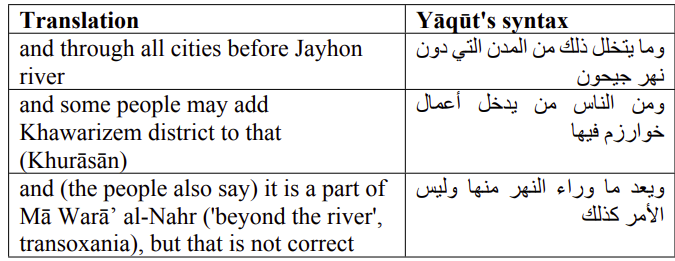
\includegraphics[width=0.7\linewidth]{figures/yaqut-with-translation} % Include the image with desired width
    \caption{Original, Arabic entries from Kitāb Mu'jam al-Buldān with their corresponding English tranlations~\cite{YaqutRB}} % Add a caption
    \label{fig:yaqut-entries} % Assign a label for referencing the figure in text
\end{figure}.

\subsection{Parsed Dataset - Places}
The layout of the gazetteer is highly structured, therefore, researchers were able to create a rule based method to parse
and expose the data in a tabular database~\cite{YaqutRB}.
This database provides serves as the primary datasource for this thesis.

\begin{figure}[h] % [h] attempts to place figure here, other options like [t]op, [b]ottom
    \centering % Centers the figure horizontally
    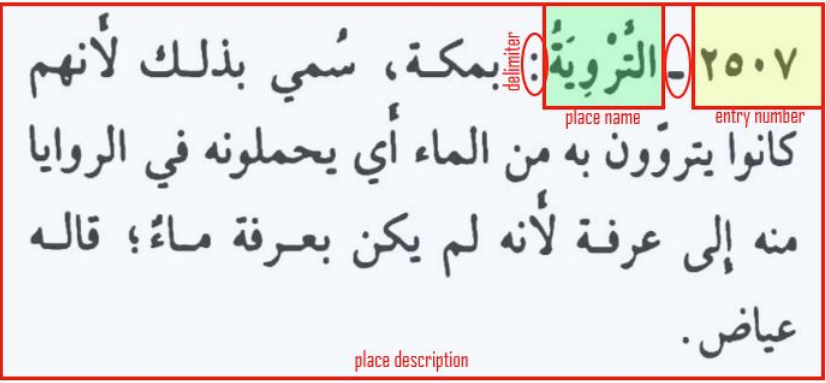
\includegraphics[width=0.8\linewidth]{figures/yaqut-layout} % Include the image with desired width
    \caption{Example of Muʿjam al-Buldān entry ~\cite{YaqutRB}} % Add a caption
    \label{fig:yaqut-structure} % Assign a label for referencing the figure in text
\end{figure}.

The primary, parsed datasource provided the following information:
\begin{itemize}
    \item Latitude
    \item Longitude
    \item Wikidata ID
    \item al-Turayyā ID~\cite{AlTurayya}
    \item Name (Arabic)
    \item Name (English)
    \item Type (lower hierarchy)
    \item Type (upper hierarchy)
    \item Metropolitan ID (reference to another place in the dataset)
    \item District ID (reference to another place in the dataset)
    \item Provincial ID (reference to another place in the dataset)
\end{itemize}


The only fields guaranteed to have data were the Arabic name and the unique identifier assigned based on the corresponding al-Turayyā gazetteer~\cite{AlTurayya}.

\subsubsection{al-Turayyā ID}
The IDs correspond to the database entries partially backing the al-Turayyā gazetteer project.
Namely, al-Turayyā used the same IDs to identify the OCR scanned entries.
A small caveat is that~\cite{YaqutRB} occasionally parsed multiple place descriptions from the same entry,
therefore, these entries have additional suffixes after the al-Turayyā ID to keep them unique.

\subsubsection{Wikidata ID}
Some more well known and easily identifiable place entries such as Baghdad were already enriched with Wikidata~\cite{Wikidata} IDs.
This information was initially used to build some graphs, but later iterations forewent its use due to the unreliability.
As an example, the entry for Mecca, which is a highly central and important node had the Wikidata ID of Q3289054
which refers to a city in the United States, not to the Saudi Arabian city.

\subsubsection{Categories}
The rule based parsing system also attempts to assign a category to each place entry.
The categories are selected from a pre-defined hand verified list.

The categories are split into a two level hierarchy.
For example, the level one category "town" has multiple sub-categories, like
village, small town, neighboring villages or abodes.

However, not all entries necessarily will have a secondary category.
In total there are 96 distinct categories.

\subsection{Parsed Dataset - Distances}
The other important block of data available in the parsed dataset are the distances.
There are over a thousand entries parsed from the original book, that express some spatial relationship
between two places.

The dataset this thesis works with, already contains this information in kilometres, but it is important
to keep in mind that the kilometer values provided are highly varying in terms of accuracy. This
is due to the fact that the original entries defined distance in terms of various non-standard methods
such as days of walking, travelling on camel back and so on.




\section{Relevant Concepts and Technologies}\label{sec:relevant-concepts}

\subsection{Knowledge Graphs}\label{subsec:introduction-knowledge-graphs}

\begin{wrapfigure}{r}{0.5\textwidth} % Float right, width half the text width
    \centering
    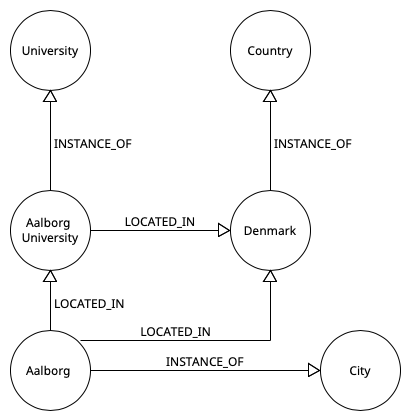
\includegraphics[width=\linewidth, scale=0.5]{figures/kg-example}
    \caption{Example of a knowledge graph.}
    \label{fig:kg-example}
\end{wrapfigure}
While there is no formal, widely accepted definition of Knowledge Graphs, one may think of them as a directed heterogeneous graphs
created with the intent of representing knowledge bases in a machine interpretable manner.

Nodes may (but not bound to) be objects, events, situations, abstract concepts or locations,
with the edges between the nodes representing conceptual relationships among the entities.

Knowledge graphs are often represented as lists of statements such that a statement is: $s = (h,r,t)$
where $h$ refers to the head entity, $t$ represents the tail entity and $r$ represents the
edge connecting the two entities.
These statements have also been called triplets.


Knowledge graphs are often backed by predefined ontologies.
Ontologies define entities and relationships referenced in the list of statements.
serving as their explicit schema, making the parsing of and
work with these graphs easier.

One may also think of knowledge graphs as the combination of the statements, and the relevant ontologies.

Some use cases of knowledge graphs include Google's enhanced contextual response to search queries~\cite{GoogleKnowledgeGraph} (using their internal
knowledge graph) or a more recent example: researchers have been experimenting with augmenting large language models
with knowledge graphs~\cite{LLMKG}, in order to ensure factual answers.

Examples of publicly available knowledge graphs are: Wikidata~\cite{Wikidata} a generic
knowledge graph backing the rest of the Wikimedia ecosystem, or WN18 dataset parsed from WordNet
introduced by~\cite{TransE} and is commonly used to evaluate the performance of various graph machine learning models.



\FloatBarrier
\subsection{Graph Representation Learning}\label{subsec:introduction-graph-representation-learning}
Graph Representation Learning is a research field dedicated to create various methods of embedding nodes of a graph into
a low dimensional vector space that may be used to perform various downstream tasks such as graph and node classification, or link prediction.

These GRL models rely on an encoder-decoder model.
"The intuition behind the encoder-decoder idea is the following:
if we can learn to decode high-dimensional graph information—such as the global positions of
nodes in the graph or the structure of local graph neighborhoods—from encoded low-dimensional embeddings, then, in principle,
these embeddings should contain all information necessary for downstream machine learning tasks"~\cite{RLGMandA}

In other words, while downstream tasks consume the vector representation, the decoder is used to create a well-trained encoder model.

The encoder may create either shallow embeddings, or deep embeddings.
Shallow embedding techniques are generally simpler and faster to train, but
may struggle to capture highly complex patterns and hierarchical relationships within the graph.

Example of shallow embedding methods include: Node2Vec~\cite{Node2vec} or DeepWalk~\cite{DeepWalk}

Deep embedding methods are commonly some variation of Graph Neural Networks detailed in section~\ref{subsec:introduction-graph-neural-networks}

\subsection{Graph Neural Networks}\label{subsec:introduction-graph-neural-networks}
The challenge in creating encoding models that capture deep insight into graph structures, is that graph structures are inherently variable ~\cite{GRLBook}.

For example, if one was to build a model that categorizes social networks using classical tools such as Convolutional Neural Networks or Recurring Neural Networks,
the model would be restricted to graphs with a set amount of nodes.

To address the above issue, and the leverage the structure of graphs Graph Neural Networks are used, which leverage the concept of Neural Message Passing.
The recent state-of-the art knowledge graph completion models are commonly based on some neural message passing framework~\cite{LPSOTA}, due to their inherent ability to capture
deeper neighborhood structures.

\begin{figure}[h] % [h] attempts to place figure here, other options like [t]op, [b]ottom
    \centering % Centers the figure horizontally
    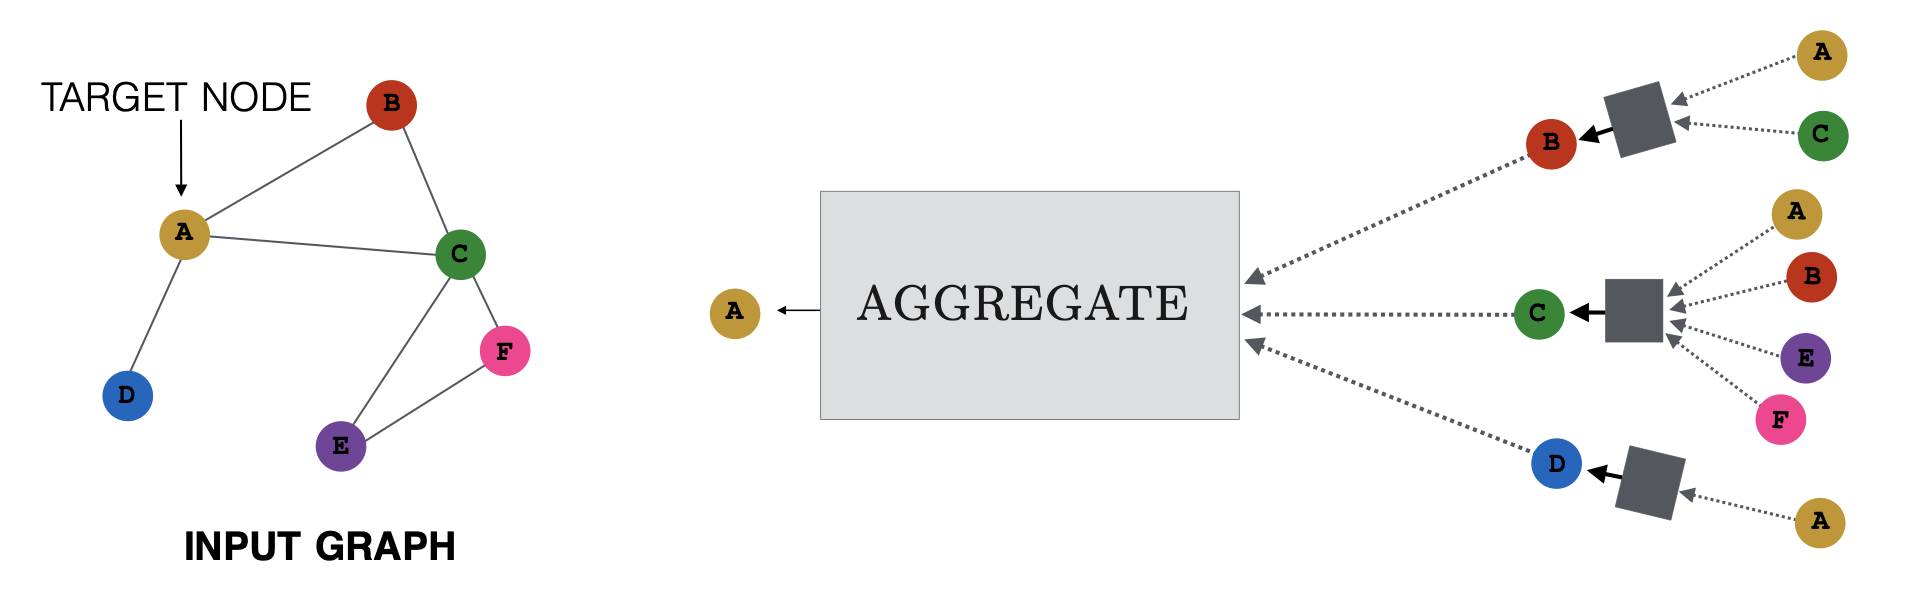
\includegraphics[width=0.9\linewidth]{figures/gnn} % Include the image with desired width
    \caption{A figure from the book, Graph Representation Learning~\cite{GRLBook} showcasing the general intuition behind neural message passing.} % Add a caption
    \label{fig:gnn} % Assign a label for referencing the figure in text
\end{figure}


\subsection{Wikidata}\label{subsec:introduction-wikidata}
"Wikidata is a free, collaborative, multilingual, secondary knowledge base, collecting structured data to provide support for Wikipedia, Wikimedia Commons, the other wikis of the Wikimedia movement,
and to anyone in the world."

"The Wikidata repository consists mainly of items, each one having a label, a description and any number of aliases.
Items are uniquely identified by a Q followed by a number, such as Douglas Adams (Q42).
Statements describe detailed characteristics of an Item and consist of a property and a value.
Properties in Wikidata have a P followed by a number, such as with educated at (P69)."~\cite{Wikidata}

As detailed later in section~\ref{sec:graph-building} the initial dataset that forms the basis of this thesis contains a number of nodes that have inferred Wikidata Ids.
Therefore, Wikidata will be used as a potential source for enriching the dataset, creating a denser network.

Moreover, a secondary object of this thesis is to represent Kitāb Mu'jam al-Buldān in a consumable knowledge graph format.
Therefore, it is easy to argue that using Wikidata's ontology will streamline such efforts.

\subsection{Neo4j}\label{subsec:introduction-neo4j}
During the development stages of this thesis, a heavily used tool was Neo4J~\cite{Neo4j}.
Neo4J is a No-SQL database engine, designed to store and manipulate graph-like structures.
The end user may access and modify the data via Neo4J's custom query language - Cypher.

While other similar graph database engines are available and would have been sufficient, this project uses Neo4J
due to its wide adoption and subsequent easy of access to relevant information.



\chapter{Building the Initial Graph and its Analysis}\label{ch:graph-analisys}

\section{Building the Graph}\label{sec:graph-building}
Within this thesis, there are two target edge categories that are valuable to predict: distance, and hierarchy.
Therefore, it is reasonable to create an initial investigative graph containing this information.

The graph will contain only place nodes, one node for each unique place ID. For simplicity, the distance edges
will not yet be binned, and each hierarchical relationship will explicitly be defined instead of relying on meta-paths.

The database engine storing the graph will be Neo4J, populated by a Python script while the analysis will be mainly done
with Gephi~\cite{Gephi}.

While building the graph, it became apparent that the number of disconnected nodes are exceedingly high (6289 nodes are orphans out of 14863 total nodes), therefore
the decision was made to only consider connected nodes as part of the graph, especially since the link prediction methods
require at least some connections.

\section{Initial Analysis}\label{sec:initial-analysis}
\subsection{Network Density and Connectivity}\label{subsec:network-density-and-connectivity}


Even with the disconnected nodes removed, the graph appears to be extremely sparse.
This is apparent from the density, which  may be calculated as follows:
\[
    D = \frac{2E}{N(N - 1)}
\]

With 8574 nodes and 10790 edges, the density is $~0.00029$.
Considering that a graph's density such that: ($0 \leq density \leq 1$), this graph is rather disconnected.

\subsection{Average Degree and Degree Distribution}\label{subsec:average-degree-and-degree-distribution}
The average degree of a node is 1.258, which again reinforces the perception of a sparse graph.
This low density may cause problems down the line, as link prediction methods commonly perform better on denser graphs.

The degree distribution (figure~\ref{fig:degree-distribution})
shows that there are a few nodes in the graph that are exceedingly central
(upwards of 6000 edges).
After some investigation,
it was found that these nodes generally correspond to large medieval cities or countries such as Baghdad,
Alexandria or Yemen.

Besides these highly central nodes, the degree distribution is fairly spread out.

\begin{figure}[h] % [h] attempts to place figure here, other options like [t]op, [b]ottom
    \centering % Centers the figure horizontally
    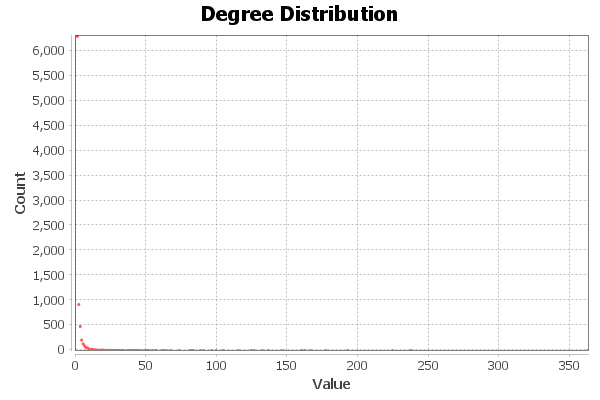
\includegraphics[width=1\linewidth]{figures/degree-distribution/degree-distribution} % Include the image with desired width
    \caption{Degree Distribution of the Initial Graph} % Add a caption
    \label{fig:degree-distribution} % Assign a label for referencing the figure in text
\end{figure}


\subsection{Modularity}\label{subsec:modularity}
Using Gephi's~\cite{Gephi} implementation of the Louvian method~\cite{Louvian} with a resolution of 5.0,
217 communities were found.

However, the high number of communities is only indicative of a highly disconnected graph, with many small, isolated node islands.
In practice there are 8 large groups accounting for 94.62\% of the nodes.

The modularity breakdown is shown on table:~\ref{tab:luv-communities}


\begin{table}[]
\centering
\begin{tabular}{|l|l|l|}
\hline
\textbf{Name} & \textbf{Population} & \textbf{Color on Figure ~\ref{fig:communities}} \\ \hline
Group 1       & 22.26\%             & Pink                     \\ \hline
Group 2       & 17.46\%             & Green                    \\ \hline
Group 3       & 15.13\%             & Blue                     \\ \hline
Group 4       & 9.41\%              & Black                    \\ \hline
Group 5       & 9\%                 & Orange                   \\ \hline
Group 6       & 8.69\%              & Red                      \\ \hline
Group 7       & 6.85\%                & Yellow                   \\ \hline
Group 8       & 5.82\%                & Cyan                     \\ \hline
\end{tabular}
\caption{Communities ratios detected by the Louvain method}
\label{tab:luv-communities}
\end{table}

Figure~\ref{fig:communities} shows that the detected, large communities are fairly easy to visually distinguish.
Moreover, it shows that the highly central nodes (visualized via larger diameter) are spread around the communities fairly evenly.

\begin{figure}[h] % [h] attempts to place figure here, other options like [t]op, [b]ottom
    \centering % Centers the figure horizontally
    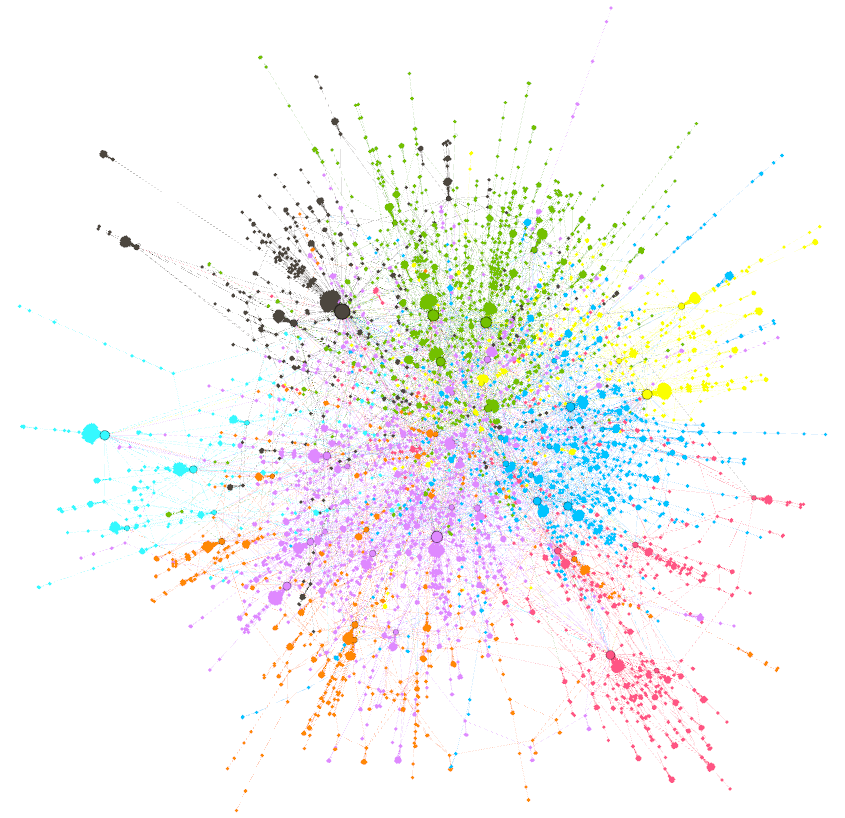
\includegraphics[width=0.7\linewidth]{figures/modules} % Include the image with desired width
    \caption{Graph visualization showing the communities listed on table~\ref{tab:luv-communities}} % Add a caption
    \label{fig:communities} % Assign a label for referencing the figure in text
\end{figure}.


\subsection{Unexpected Patterns}\label{subsec:odd-patterns}

While working with the parsed dataset, some odd patterns were found.
First, \textbf{DISTANCE} triplets were found, where both the head and tail entity were the same.
At the recommendation of the authors of ~\cite{YaqutRB} these triplets were discarded.



\begin{figure}[h] % [h] attempts to place figure here, other options like [t]op, [b]ottom
    \centering % Centers the figure horizontally
    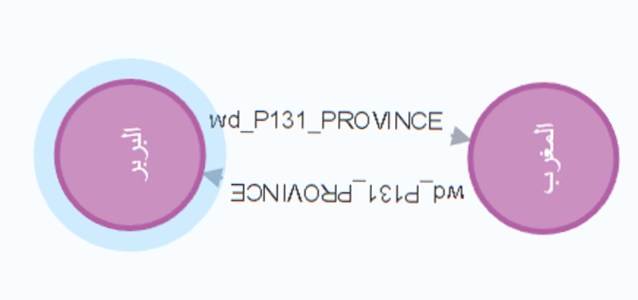
\includegraphics[width=0.5\linewidth]{figures/odd1} % Include the image with desired width
    \caption{Unusual hierarchical pattern where two nodes reference each other as their province.} % Add a caption
    \label{fig:odd1} % Assign a label for referencing the figure in text
\end{figure}

Secondly, during manual observation of the data, "odd" hierarchical patterns were observed;
that did not fit to the classical strict, unidirectional layout of other similar structures, shown on figure~\ref{fig:odd1} and ~\ref{fig:odd2} .

\begin{figure}[h] % [h] attempts to place figure here, other options like [t]op, [b]ottom
    \centering % Centers the figure horizontally
    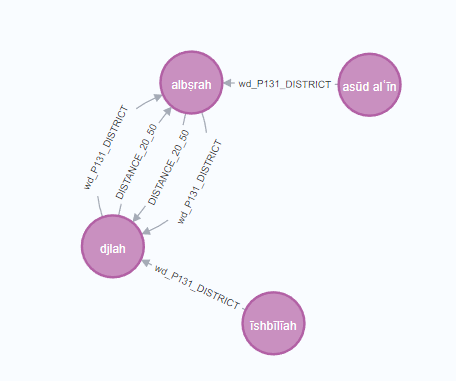
\includegraphics[width=0.5\linewidth]{figures/odd2} % Include the image with desired width
    \caption{Unusual hierarchical pattern where two nodes reference each other as their district.} % Add a caption
    \label{fig:odd2} % Assign a label for referencing the figure in text
\end{figure}

These patterns were extracted and forwarded to the Mehdie researchers using the following Neo4J query:
\begin{verbatim}
    MATCH (n)-[:{r1}]->(m)-[:{r2}]->(n) RETURN n,m
\end{verbatim}

Where r1 and r2 correspond to all potential pairwise combinations of the edge types:
\textbf{wd\_P131\_METROPOLITAN}, \textbf{wd\_P131\_DISTRICT} and \textbf{wd\_P131\_PROVINCE}


\chapter{Knowledge Graph Embedding Methods}\label{ch:knowledge-graph-embedding-methods}
The first broad classification of link prediction methods explored in this thesis are the knowledge graph embedding methods (KGE).
Since graph neural networks generate node embeddings as well, the terminology is somewhat ambiguous.
The following few paragraphs will attempt to clearly distinguish the class of methods detailed in this chapter.

KGE methods attempt to position each node in a vector space (figure~\ref{fig:vec-space-vis}).
In a well-trained model, nodes from the same neighborhood will be placed near each other within the vector space.
Moreover, these positions are strictly unique, i.e.\ two distinct nodes cannot occupy the same place.
From this, naturally follows that KGE methods are strictly transductive, and cannot generalize.

Fortunately, a transductive setting is not necessarily limiting for the purposes of this thesis.
(TODO: WorldKG), as all the link-predictions tasks are limited
to the domain of places mentioned in Kitāb Mu'jam al-Buldān.

While there are exceptions to this rule, such as the ComplEx~\cite{ComplEx} discussed in TODO: ComplexRef
KGE methods are generally more efficient and easily more scalable than their GNN counterparts.
\begin{figure}[h] % [h] attempts to place figure here, other options like [t]op, [b]ottom
    \centering % Centers the figure horizontally
    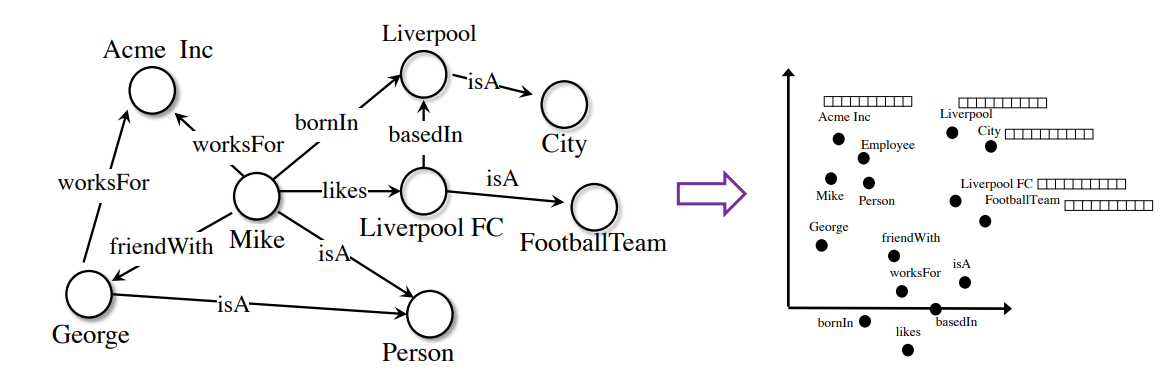
\includegraphics[width=1\linewidth]{figures/vector-space} % Include the image with desired width
    \caption{Visualization of Vector Space Embedding~\cite{KGETutorial}} % Add a caption
    \label{fig:vec-space-vis} % Assign a label for referencing the figure in text
\end{figure}.
\section{General Architecture}
Generally, KGE models, at least within the context of this thesis, fit into the same generic architecture (figure~\ref{fig:kge-architecture}).

\begin{figure}[h] % [h] attempts to place figure here, other options like [t]op, [b]ottom
    \centering % Centers the figure horizontally
    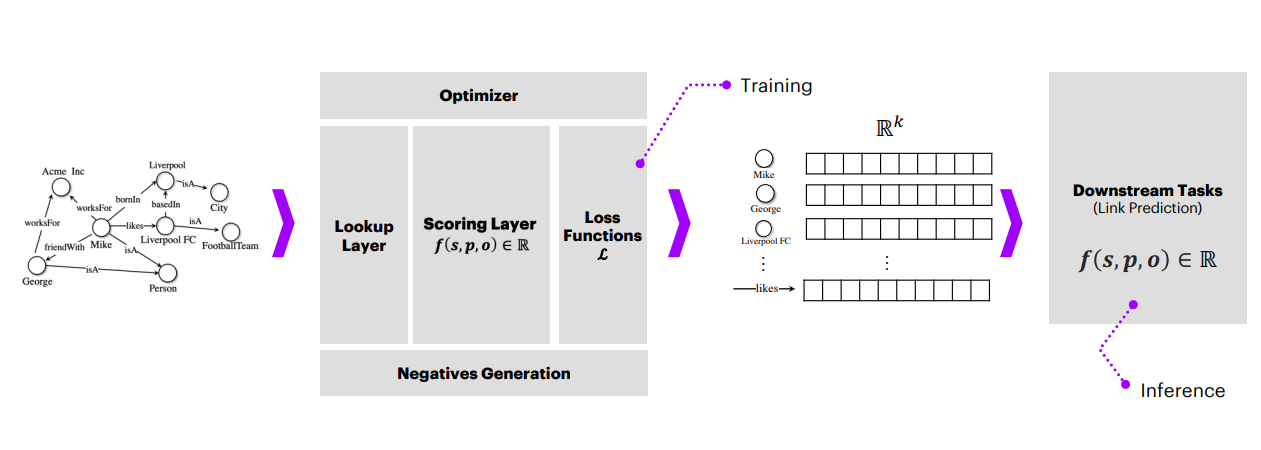
\includegraphics[width=1\linewidth]{figures/kge-architecture} % Include the image with desired width
    \caption{Generic KGE architecture~\cite{KGETutorial}} % Add a caption
    \label{fig:kge-architecture} % Assign a label for referencing the figure in text
\end{figure}.

\subsection{Lookup Layer}
The Lookup layer just simply functions as a dictionary between the individual nodes and relationships and their respective embeddings.
\subsection{Scoring Layer}
Colloquially, the heart of the architecture, the scoring layer takes the encoding of each member of the triplet
and assigns a score to the whole statement.
The higher the score, the more likely it is that the statement is a true statement.
The specific scoring functions are detailed in section~\ref{sec:embedding-methods}

\subsection{Loss Function}
As with all other neural models; the generic KGE architecture relies on a loss function, which is necessary to optimize the model.
In the KGE section of this thesis, two loss functions were used.

\subsubsection{Pairwise, Max-margin Loss}
This function penalizes the model if the score assigned by scoring function $f_{model}$
to a positive triple $t^+$ selected from the set of positives $\mathcal{G}$, is lower than the score assigned to a
negative triple $t^-$ selected from the set of corruptions $\mathcal{C}$
by margin $\gamma$

\begin{gather*}
    \mathcal{L}(\Theta) = \sum_{t^+ \in \mathcal{G}}\sum_{t^- \in \mathcal{C}}max(0, [\gamma + f_{model}(t^-;\Theta)
 - f_{model}(t^+;\Theta)])
\end{gather*}

\subsubsection{Negative Log-Likelihood Loss}
Another commonly used loss function, $y \in -1,1 $ dependent on whether the statement is positive or negative.
\begin{gather*}
    \mathcal{L}(\Theta) = \sum_{t \in \mathcal{G} \cup \mathcal{C}}log(1 + exp(-y \, f_{model}(t;\Theta)))
\end{gather*}

\subsection{Negatives Generation}\label{subsec:negatives-generation}
A very distinctive feature of the domain of knowledge graph link prediction is the (usual) lack of true negative data points.
Let's consider the domain of image recognition.
If someone were to train a model to detect the presence of a cat in a photo,
the negative data points could be any photos that do not contain a cat.
However, in the case of knowledge graphs, there are no negative facts.
A knowledge graph may contain the triplet \textit{<London,CapitalOf,UnitedKingdom>}

And even though for a human reader, this automatically means that \textit{<London, CapitalOf, Denmark>} is a false statement,
a normal knowledge graph will not contain such information explicitly.
Therefore, link prediction methods commonly rely on some form of synthetic negative triplet generation.

While there have been many strategies proposed~\cite{NegSamp}, in this thesis, a very simple method was chosen.
Given a true statement $s = (h,r,t)$, a negative sample will be generated by corrupting $t$ by randomly replacing it with another node from the graph.
Of course, corruption is done with consideration of the ground truth triplets.

This has a negative effect under the open world assumption
of potentially labeling unknown true positives as negative data points ~\cite{OpenWorld}.
However, due to its simplicity, this approach has the benefit of avoiding any potential bias in the training
and being computationally efficient.

\subsection{Optimizer}
Same concept as in other machine learning architectures, in this thesis two optimizers were used:
Adam~\cite{Adam} and AdaGrad~\cite{Adagrad}


\section{Embedding Methods}\label{sec:embedding-methods}
\subsection{Translating Embeddings (TransE)}
Commonly used benchmark, and one of the first KGE models.
This approach attempts to model relationships as translations between two points (nodes) in a vector space

Given a statement $s = (h,r,t)$, ideally $h$ and $t$ should be close to each other in the vector space,
with the difference being the translation of the relation $r$~\cite{TransE}.


\begin{figure}[h] % [h] attempts to place figure here, other options like [t]op, [b]ottom
    \centering % Centers the figure horizontally
    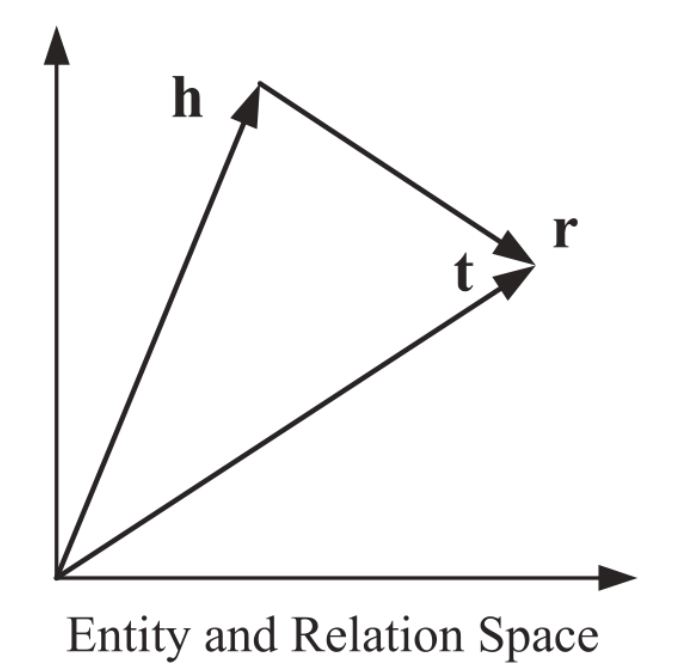
\includegraphics[width=0.35\linewidth]{figures/transe} % Include the image with desired width
    \caption{Visualization of TransE~\cite{TransEFig}}
    \label{fig:transe-example}
\end{figure}.

\FloatBarrier

\subsection{Relational Rotation Embeddings (RotatE)}
"The RotatE model maps
the entities and relations to the vector space and defines each relation as a rotation from
the source entity to the target entity."~\cite{RotatE}

The benefit of RotatE over TransE lies in expressiveness.
It is able to model more relationship patterns, such as symmetry, antisymmetry, inversion
and composition.

\begin{figure}[h] % [h] attempts to place figure here, other options like [t]op, [b]ottom
    \centering % Centers the figure horizontally
    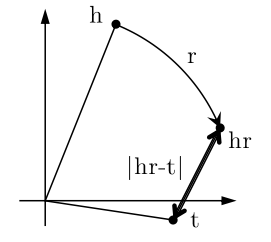
\includegraphics[width=0.35\linewidth]{figures/rotate} % Include the image with desired width
    \caption{Visualization of RotatE~\cite{RotatE}}
    \label{fig:rotate}
\end{figure}.

\FloatBarrier


\subsection{Holographic Embeddings (HolE)}

Holographic Embedding~\cite{HolE} is a model for learning representations of entities and relationships in a knowledge graph.
It uses the principles of holography and circular correlation to combine entity embeddings in a way that captures rich
interactions between entities and relations.

The main benefit of HolE over other approaches is the increased modeling power.

\subsection{The Bilinear Diagonal DistMult Model (DistMult)}

DistMult is a tensor factorization based model introduced in~\cite{DistMult} that uses,
trilinear dot product as its scoring function.

However, a big limitation of DistMult is that it cannot model asymmetric relationships.

\subsection{Complex Embeddings (ComplEx)}

ComplEx~\cite{ComplEx} is similar to DistMult in using the dot product of two vectors to calculate the score.
However, it uses the Hermitian dot product, which is able to handle asymmetrical relationships.

Moreover, instead of using real-valued vectors, DistMult uses a complex vector space for both entities and relations.
Allowing to capture richer information about the graph at the cost of increased computational cost.

\subsection{Benchmark Comparison of KGE Methods}
Table~\ref{tab:kge-perf-comp} shows the performance of the above detailed KGE methods on the FB15k benchmark dataset.


\begin{table}[!ht]
    \centering

    \begin{tabular}{|l|l|l|l|}
        \hline
         & MRR            & Hits@1                       & Hits@10               \\ \hline
TransE   & 0.463          & 0.29                         & 0.75                  \\ \hline
RotatE   & 0.797          & \textbf{0.746}               & 0.884                 \\ \hline
HolE     & 0.524          & 0.4                          & 0.73                  \\ \hline
DistMult & \textbf{0.841} &                              & \textbf{0.914}        \\ \hline
ComplEx  & 0.84           & 0.692 &  0.75                                        \\ \hline
\end{tabular}
\caption{Performance of Discussed KGE Methods on the FB15k Benchmark Dataset. Datasources~\cite{paperswithcode2024fb15k, HolE}}
\label{tab:kge-perf-comp}
\end{table}

\section{Methodology}
In the initial KGE experiments, the dataset generated in TODO was used as data for the models.
The dataset was split into train, test and validation dataset in a $80\%$, $10\%$ and $10\%$ ratio.
The split was done in a transductive manner, such that there are no, previously unseen nodes in the test and validation
dataset.

To find the best performing model and the most optimal hyperparameters, a grid search was performed, with the MRR score
being the basis of comparison.

For each method detailed in section TODO, the following hyperparameters were tuned:
\begin{itemize}
    \item \textbf{Batch size:} 128, 256, 512, 1024, 2048
    \item \textbf{Epochs:} 5, 25, 50, 100, 200, 250
    \item \textbf{Eta:} 5, 10, 15 (\textit{eta specifies the number of corruptions to generate per each positive})
    \item \textbf{Vector embedding size:} 50, 100, 150, 200
    \item \textbf{Loss function:} pairwise, nll
    \item \textbf{Optimizer:} AdaGrad, adam
\end{itemize}

The best performing model and hyperparameter combinations are shown on table~\ref{tab:kge-params}.

\begin{table}[!ht]
    \centering
    \begin{tabular}{|l|l|l|l|l|l|}
        \hline
        & \textbf{TransE} & \textbf{RotatE} & \textbf{HolE} & \textbf{DistMult} & \textbf{ComplEx} \\ \hline
        \textbf{Batch size} & 2048 & 1024 & 128 & 128 & 128 \\ \hline
        \textbf{Epochs} & 200 & 90 & 80 & 60 & 50 \\ \hline
        \textbf{k} & 150 & 150 & 200 & 200 & 200 \\ \hline
        \textbf{eta} & 5 & 15 & 5 & 5 & 5 \\ \hline
        \textbf{loss} & pairwise & nll & pairwise & pairwise & pairwise \\ \hline
        \textbf{optimizer} & adam & adam & adam & adam & adam \\ \hline
    \end{tabular}
    \caption{Best performing KGE hyperparameters}
    \label{tab:kge-params}
\end{table}
\section{Results}
Unfortunately, even with the tuned hyperparameters, the KGE models produced subpar results (table~\ref{tab:kge-res}).
With the highest MRR being $0.18$ produced by HolE, DistMult and ComplEx with DistMult slightly under-performing in
hits@10 compared to the other two.
\begin{table}[!ht]
    \centering
    \begin{tabular}{|l|l|l|l|l|}
        \hline
         & MRR & Hits@10 &  Hits@5 &  Hits@1 \\ \hline
        TransE & 0.11   & 0.24 & 0.14 & 0.04 \\ \hline
        RotatE & 0.16   & 0.21 & 0.17 & 0.13 \\ \hline
        HolE & 0.18     &  0.22 & 0.19 & 0.16 \\ \hline
        DistMult & 0.18 & 0.21 & 0.18 & 0.16 \\ \hline
        ComplEx & 0.18  & 0.22 & 0.19 & 0.16 \\ \hline
    \end{tabular}
    \caption{Performance of the hyperparameter tuned KGE models on a previously unseen test dataset}
    \label{tab:kge-res}
\end{table}

After some investigation, two apparent issues were found.
First, the kilometer values of distance edges range from ~1 kilometer to over 1000 kilometers.
Therefore, all the distance edges were binned into ranges.

Second, the model was incorrectly predicting not explicitly defined hierarchical information.
Since this information was available in the source dataset, it made sense to modify the training data
to include all available hierarchical information instead of expecting the model to learn the hierarchical meta-paths.

Finally, reverse edge types were introduced to increase the graph density.
These edges were only inserted after the train / test / validation split to avoid leakage.

The final edge composition in the data is shown on table~\ref{tab:kge-new-edges} (excluding the reverse edge counts
as they are obviously equal to their counterparts.).

\begin{table}[!ht]
    \centering
    \begin{tabular}{|l|l|}
        \hline
        \textbf{Edge Type } & \textbf{Count} \\ \hline
        DISTANCE\_0\_5 & 50 \\ \hline
        DISTANCE\_5\_10 & 48 \\ \hline
        DISTANCE\_10\_20 & 254 \\ \hline
        DISTANCE\_20\_50 & 690 \\ \hline
        DISTANCE\_50\_100 & 340 \\ \hline
        DISTANCE\_100\_200 & 294 \\ \hline
        DISTANCE\_200\_500 & 142 \\ \hline
        DISTANCE\_500\_1000 & 6 \\ \hline
        DISTANCE\_1000\_inf & 8 \\ \hline
        wd\_P17 & 3507 \\ \hline
        wd\_P31 & 13707 \\ \hline
        wd\_P131\_DISTRICT & 3124 \\ \hline
        wd\_P131\_METROPOLITAN & 4695 \\ \hline
        wd\_P131\_PROVINCE & 4252 \\ \hline
        wd\_P279 & 66 \\ \hline
        wd\_P206 & 223 \\ \hline
        wd\_P361 & 287 \\ \hline
        wd\_P706 & 57 \\ \hline
    \end{tabular}
    \caption{Edge Count of the Second Iteration of the KGE Experiments}
    \label{tab:kge-new-edges}
\end{table}

With the new training dataset, the hyperparameter tuning was repeated for each method.
Unfortunately it appears that the new dataset did not result in increased model performance.
In fact all across the board, the performance of the models decreased (table~\ref{tab:kge-new-res}).

However, it is important to point out that some of the reduction in performance may be attributed to the increased
difficulty in distance prediction.

\begin{table}[!ht]
    \centering
    \begin{tabular}{|l|l|l|l|l|}
        \hline
        & MRR & Hits@10 &  Hits@5 &  Hits@1 \\ \hline
        TransE & 0.09   & 0.24 & 0.12 & 0.037 \\ \hline
        RotatE & 0.07   & 0.14 & 0.09 & 0.039 \\ \hline
        HolE & 0.12     &  0.19 & 0.16 & 0.09 \\ \hline
        DistMult & 0.16 & 0.22 & 0.19 & 0.12 \\ \hline
        ComplEx & 0.16  & 0.22 & 0.2 & 0.13 \\ \hline
    \end{tabular}
    \caption{Performance of the hyperparameter tuned KGE models on a previously unseen test dataset}
    \label{tab:kge-new-res}
\end{table}

\chapter{Experiments with Neural Bellman-Ford Networks}\label{ch:nbfnet}


\section{Introduction}\label{sec:nbfnet-introduction}
After the lackluster result from the translation methods detailed in chapter~\ref{ch:knowledge-graph-embedding-methods}, the need for
experimentation with other approaches became apparent.

At the time of writing, the state-of-the art multi-relational link prediction methods~\cite{LPSOTA} are generally
based on, and expand on the message passing, Graph Neural network architecture.

Specifically, the top performing model, according to the Papers with Code benchmark on FB15k-237 link prediction~\cite{NBFNetSota}
are the Neural Bellman-Ford Networks (NBFNet).

Therefore, from now on, this thesis will focus on training an NBFNet model on the Kitāb Mu'jam al-Buldān dataset.


\section{Brief Overview of Neural Bellman-Ford Networks}\label{sec:nbfnet-description}
\subsection{Generalization of Graph Heuristics}\label{subsec:generalization-of-graph-heuristics}

The first intuition behind NBFNet is that many of the traditional graph heuristics such as Katz-Index, Personalized PageRank~\cite{Page1998PageRank}
or Graph Distance can be generalized into a \textit{multiplication} and a \textit{summation} step.

\begin{figure}[h] % [h] attempts to place figure here, other options like [t]op, [b]ottom
    \centering % Centers the figure horizontally
    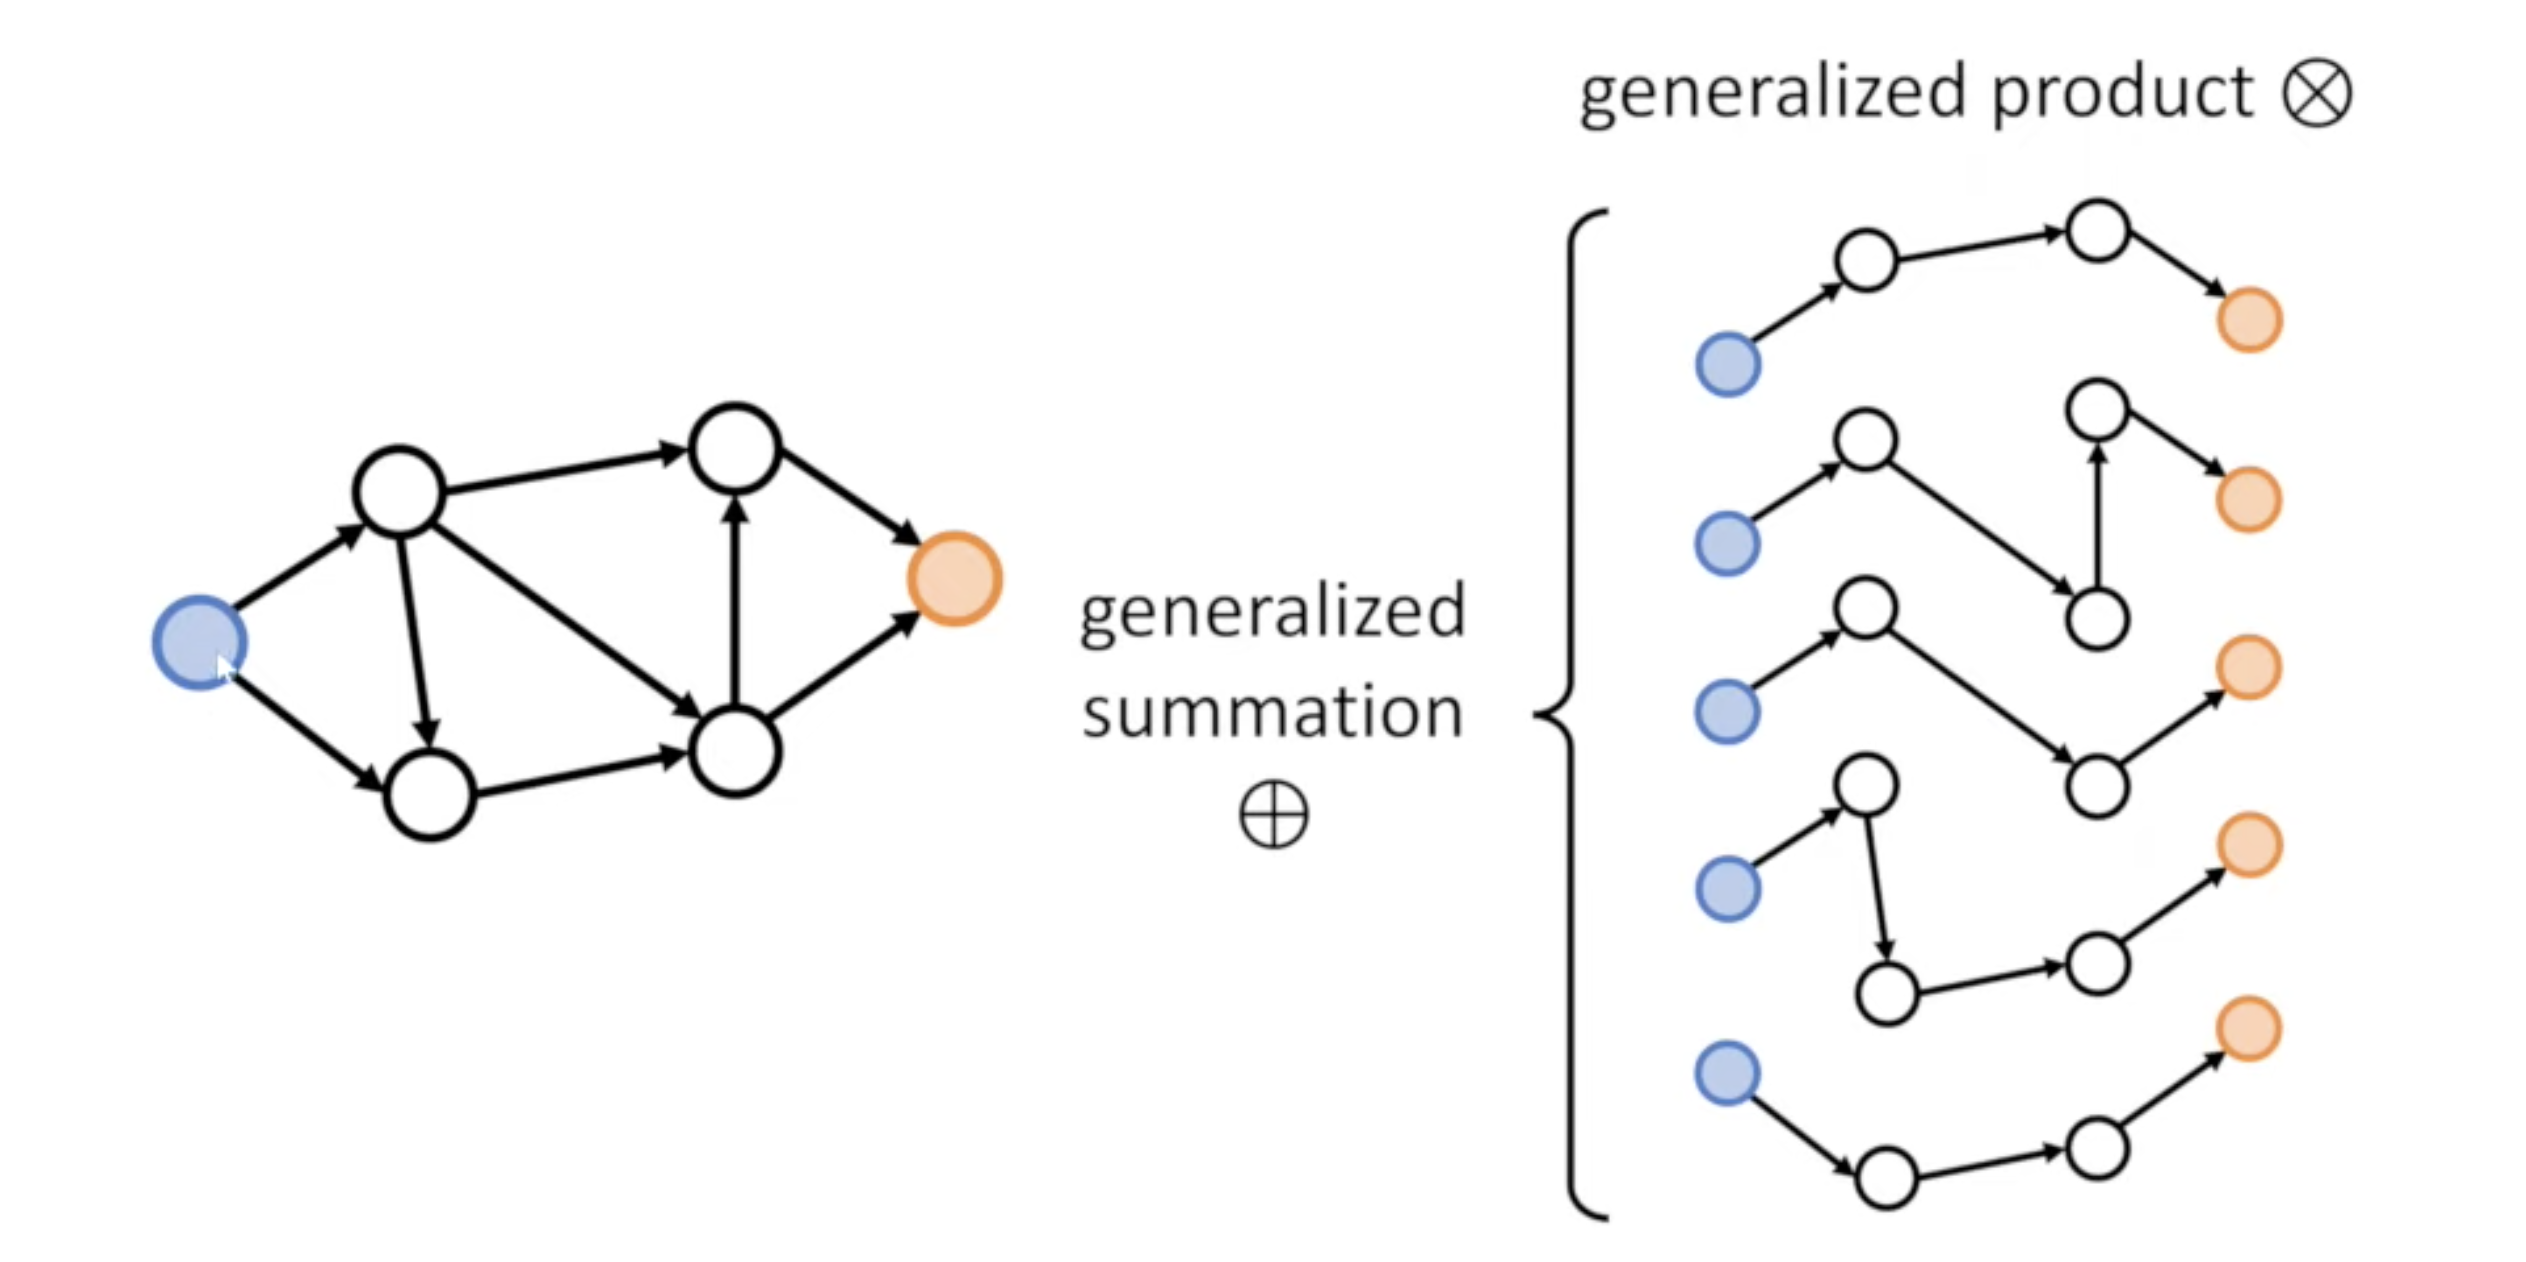
\includegraphics[width=0.8\linewidth]{figures/nbfnet-trad} % Include the image with desired width
    \caption{Generalized Graph Heuristic ~\cite{NBfnetPres}} % Add a caption
    \label{fig:nbfnet-trad} % Assign a label for referencing the figure in text
\end{figure}

For example, to find the shortest Graph Distance between two nodes, first we count the number of hops (generalized multiplication step by count) and then we select
the path with the fewest hop (generalized summation via the min function)

The second intuition behind NBFNet is that traditional link prediction methods that rely on encapsulating local neighborhoods~ ~\cite{RandomWalks, SubgraphExtraction}
perform random walks between the source and the target node.

Instead of these random walks, the pair representation can be formulated as "a generalized sum of path representations between u and v with a commutative
summation operator \bigoplus"~\cite{NBFNet}.

Within this summation, each path "is defined as a generalized product of the edge
representations in the path with the multiplication operator"~\cite{NBFNet}.

\subsection{Generalized Bellman-Ford Algorithm}\label{subsec:generalized-bellman-ford-algorithm}

Calculating such metrics for each node pair is computationally expensive due to its exponential nature.
As a solution, the NBFNet performs these calculations as part of a generalized Bellman-Ford algorithm, as that algorithm is highly
parallelizable (figure~\ref{fig:gen-bf}).

\begin{figure}[h] % [h] attempts to place figure here, other options like [t]op, [b]ottom
    \centering % Centers the figure horizontally
    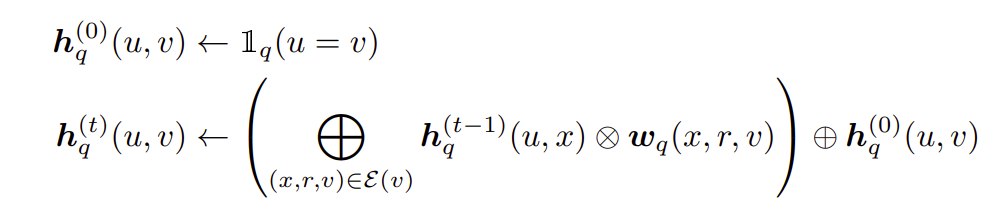
\includegraphics[width=0.8\linewidth]{figures/nbfnet-gen-bf} % Include the image with desired width
    \caption{Generalized Bellman-Ford Algorithm ~\cite{NBFNet}} % Add a caption
    \label{fig:gen-bf} % Assign a label for referencing the figure in text
\end{figure}

\subsection{Neural Bellman-Ford Networks}\label{subsec:neural-bellman-ford-networks}
Finally, to increase the potential of the models and detach from classical, handcrafted methods, the creators of NBFNet replaced
the generalized \textit{summation} and \textit{multiplication} operators with neural functions.

A Neural Bellman-Ford Network has three neural functions.

\subsubsection{The INDICATOR function}
"The INDICATOR function initializes a
representation on each node, which is
taken as the boundary condition of the generalized Bellman-Ford algorithm."~\cite{NBFNet}

It replaces the $\textbf{h}_q^{(0)}(u,v)\leftarrow\ \mathbbm{1}_q(u=v)$ step, seen on figure~\ref{fig:gen-bf}

\subsubsection{The MESSAGE function}
"The MESSAGE function replaces the binary multiplication operator \bigotimes"~\cite{NBFNet}


\subsubsection{The AGGREGATE function}
"The AGGREGATE function is a permutation invariant function
over sets that replaces the n-ary summation operator $\bigoplus$ \ldots
one may alternatively define AGGREGATE as the commutative binary operator $\bigoplus$ and apply it
to a sequence of messages." ~\cite{NBFNet}


The combination of the three neural function are shown on figure~\ref{fig:neural-bf}.

\begin{figure}[h] % [h] attempts to place figure here, other options like [t]op, [b]ottom
    \centering % Centers the figure horizontally
    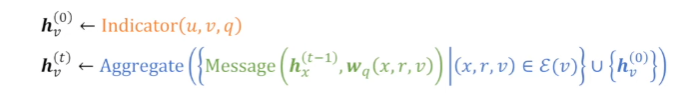
\includegraphics[width=0.65\linewidth]{figures/nbfnet-architecture} % Include the image with desired width
    \caption{Neural Bellman-Ford Network Architecture ~\cite{NBfnetPres}} % Add a caption
    \label{fig:neural-bf} % Assign a label for referencing the figure in text
\end{figure}


Finally, the learned vector representation is then fed into a multi-layer perceptron to predict the probability
of a tail node given a head node and a query relationship (figure~\ref{fig:nbfnet-mlp})

\begin{figure}[h] % [h] attempts to place figure here, other options like [t]op, [b]ottom
    \centering % Centers the figure horizontally
    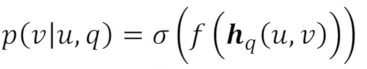
\includegraphics[width=0.4\linewidth]{figures/nbfnet-mlp} % Include the image with desired width
    \caption{Final Prediction Step in NBFNet ~\cite{NBfnetPres}} % Add a caption
    \label{fig:nbfnet-mlp} % Assign a label for referencing the figure in text
\end{figure}



\section{Methodology}\label{sec:nbfnet-methodology}
The training of the model was mainly done using the Pyg implementation of NBFNet, a codebase written by the original authors~\cite{NBFNet_PyG}.

PNA DIST mult

transductive 8-1-1 split

\section{Results}\label{sec:nbfnet-results}
Unfortunately,
the performance of the trained NBFNet model (table~\ref{tab:nbfnet-res})
on the previously unseen test dataset was comparable to
the performance of the initial KGE models.
It performed slightly worse in terms of MRR, but it achieved the highest score on Hits@10 and Hits@5

\begin{table}[!ht]
    \centering
    \begin{tabular}{|l|l|l|l|l|}
        \hline
        & MRR & Hits@10 & Hits@5 & Hits@1 \\ \hline
        TransE & 0.11   & 0.24 & 0.14 & 0.04 \\ \hline
        RotatE & 0.16   & 0.21 & 0.17 & 0.13 \\ \hline
        HolE & 0.18     &  0.22 & 0.19 & 0.16 \\ \hline
        DistMult & 0.18 & 0.21 & 0.18 & 0.16 \\ \hline
        ComplEx & 0.18  & 0.22 & 0.19 & 0.16 \\ \hline
        NBFNet & 0.17 & \textbf{0.27} & \textbf{0.21} & 0.11 \\ \hline
    \end{tabular}
    \caption{Performance of the KGE and NBFNet models}
    \label{tab:nbfnet-res}
\end{table}

A potential approach to improve the model's performance is discussed in the next chapter.
\chapter{Pretrained WorldKG NBFNet Model}\label{ch:worldkg}
The previous experiments in chapter TODO and chapter TODO show that regardless of the class of approach used,
there is a fundamental barrier when working with this thesis' knowledge graph.
Namely, there is a high chance that the sparsity of the graph prevents
any potential model from properly being able to generalize.

As a solution, this thesis proposes an alternate approach.
Instead of trying additional models, the previously used
NBFNet model could be pre-trained on a denser graph.
Since the Kitāb KG, ultimately is just the graph representation of a geospatial area,
it is relatively easy to create a synthetic dataset that mimics it.
Moreover, creating such a dataset allows for the introduction of specific distance edge biases, not generally present in Kitāb, that could provide valuable information to researchers.
Pre-training the NBFNet model on such a dataset could allow it to generalize significantly better.

A perfect source of data for creating such a synthetic dataset is WorldKG TODO cite - a research project that parsed OpenStreetMaps data into triplestore data.
The desired synthetic dataset could be created by sampling WorldKG and converting the relevant triples to use this thesis' ontology.

\section{What is WorldKG}\label{sec:what-is-worldkg}
\input{sections/chapters/worldkg/worldkg}

\section{Constructing The Dataset}\label{sec:constructing-dataset}
To construct the synthetic dataset, useful patterns need to be created first.
While it is entirely possible to create a fully connected graph, it would not represent the biases found Kitāb well.
Nodes like Alexandria are central because Yâqût found it important to define places in relation to big, central places.
Second, the local structures in Kitāb KG exist because Yâqût also found it important to define places in relation
to their surroundings.
These ideas may be boiled down into the following simple bullet points:
\begin{itemize}
    \item A nodes's local neighborhood should be well-connected.
    \item Each node should be connected to some central entity.
    \item Central entities should be connected to each other.
\end{itemize}

Following these simple rules, one could create a Kitāb KG-like synthetic dataset with higher density.
In theory, the entire WorldKG dataset could be used to create such a synthetic dataset, for practical purposes,
in reality, the data was heavily down-sampled.

\subsection{Selecting Relevant Nodes}
In WorldKG, there are over one thousand node types, most of them irrelevant to this thesis' purpose since, for example,
there were exceedingly few airports in the medieval arab world.
Instead, the categories discussed in subsection~\ref{subsec:categories} were mapped to their OSM equivalent.

Then, with Baghdad selected as the center point, all WorldKG place nodes (of relevant type) were selected in a 2000 km
radius, using the following SPARQL query:

\begin{verbatim}
SELECT ?subject ?type ?label ?wikidata ?subjectWKT ?distance
WHERE {
    # wkg:21034458 = Baghdad
    wkg:21034458 wkgs:spatialObject ?spatialObject .
   ?spatialObject geo:asWKT ?referenceWKT .

    ?subject rdf:type ?type .
    ?subject rdfs:label ?label .
    ?subject wkgs:spatialObject ?subjectSpatialObject .
    ?subjectSpatialObject geo:asWKT ?subjectWKT .
    OPTIONAL {{ ?subject wkgs:wikidata ?wikidata . }}

    FILTER (?type IN ({types}))
    BIND(geof:distance(?referenceWKT, ?subjectWKT, uom:metre) AS ?distance) .
    FILTER(?distance < 2000000).
}

\end{verbatim}
This query returned 238135 distinct nodes.
These nodes were then randomly down-sampled to 47627 entities (20\%).

\subsection{Generating Hierarchy Triplets}
The only piece of information that was not readily available in WorldKG was the hierarchical information.
Fortunately, for each node selected, there is a corresponding geometric point literal.
This point can be used to query an OSM Overpass API, such as~\cite{Overpass} to get all administrative objects
in which the point is contained.

\begin{verbatim}
is_in({x},{y})->.a;
rel(pivot.a)[boundary=administrative];
out tags center;
\end{verbatim}

The above query, written in Overpass API Query Language, among other things, gets the ID, administrative level, and
the geographical center of all enclosing administrative boundaries overlapping the parameter point.
In OpenStreetMaps, there are 11 levels of administrative hierarchy that try to represent every nation's system.
To construct the hierarchical data for the synthetic dataset, the levels were split as follows:

\begin{enumerate}
    \item $[4,3,2] \mapsto$ \textbf{wd\_P131\_PROVINCE}
    \item $[7,6,5] \mapsto$ \textbf{wd\_P131\_DISTRICT}
    \item $[11,10,9,8] \mapsto$ \textbf{wd\_P131\_METROPOLITAN}
\end{enumerate}

The logic was written such that it always tries to pick the level with the highest integer value; this was done
to increase granularity in the data.

\subsection{Generating Distance Edges}
In line with the above-detailed rules, for each node, its close neighborhood should be as dense as possible.
Therefore, for each node pair, a corresponding great circle distance was calculated.
Then, for each node, these distance edges were sampled, such that the further away the nodes were from each other,
the less likely to be sampled.

\subsection{Generating Distance Edges for Hierarchical Nodes}
To generate the distance edges between nodes that are higher in the hierarchy (i.e., more important places)
all possible pair combinations were selected.
These pairs then, without sampling, were written into triplets with the corresponding distance edge type,
selected based on the great circle distance.

\subsection{Generating Category Triplets}
In the original query, where all the nodes were selected, their types were also queried.
These can be mapped onto the Kitāb KG categories.

Finally, every node is then connected to the initial starting point, Baghdad, based on the
great circle distance.


\section{Methodology}\label{sec:worldkg-methodology}
In the initial KGE experiments, the dataset generated in TODO was used as data for the models.
The dataset was split into train, test and validation dataset in a $80\%$, $10\%$ and $10\%$ ratio.
The split was done in a transductive manner, such that there are no, previously unseen nodes in the test and validation
dataset.

To find the best performing model and the most optimal hyperparameters, a grid search was performed, with the MRR score
being the basis of comparison.

For each method detailed in section TODO, the following hyperparameters were tuned:
\begin{itemize}
    \item \textbf{Batch size:} 128, 256, 512, 1024, 2048
    \item \textbf{Epochs:} 5, 25, 50, 100, 200, 250
    \item \textbf{Eta:} 5, 10, 15 (\textit{eta specifies the number of corruptions to generate per each positive})
    \item \textbf{Vector embedding size:} 50, 100, 150, 200
    \item \textbf{Loss function:} pairwise, nll
    \item \textbf{Optimizer:} AdaGrad, adam
\end{itemize}

The best performing model and hyperparameter combinations are shown on table~\ref{tab:kge-params}.

\begin{table}[!ht]
    \centering
    \begin{tabular}{|l|l|l|l|l|l|}
        \hline
        & \textbf{TransE} & \textbf{RotatE} & \textbf{HolE} & \textbf{DistMult} & \textbf{ComplEx} \\ \hline
        \textbf{Batch size} & 2048 & 1024 & 128 & 128 & 128 \\ \hline
        \textbf{Epochs} & 200 & 90 & 80 & 60 & 50 \\ \hline
        \textbf{k} & 150 & 150 & 200 & 200 & 200 \\ \hline
        \textbf{eta} & 5 & 15 & 5 & 5 & 5 \\ \hline
        \textbf{loss} & pairwise & nll & pairwise & pairwise & pairwise \\ \hline
        \textbf{optimizer} & adam & adam & adam & adam & adam \\ \hline
    \end{tabular}
    \caption{Best performing KGE hyperparameters}
    \label{tab:kge-params}
\end{table}

\section{Results}\label{sec:worldkg-results}
Unfortunately,
the performance of the trained NBFNet model (table~\ref{tab:nbfnet-res})
on the previously unseen test dataset was comparable to
the performance of the initial KGE models.
It performed slightly worse in terms of MRR, but it achieved the highest score on Hits@10 and Hits@5

\begin{table}[!ht]
    \centering
    \begin{tabular}{|l|l|l|l|l|}
        \hline
        & MRR & Hits@10 & Hits@5 & Hits@1 \\ \hline
        TransE & 0.11   & 0.24 & 0.14 & 0.04 \\ \hline
        RotatE & 0.16   & 0.21 & 0.17 & 0.13 \\ \hline
        HolE & 0.18     &  0.22 & 0.19 & 0.16 \\ \hline
        DistMult & 0.18 & 0.21 & 0.18 & 0.16 \\ \hline
        ComplEx & 0.18  & 0.22 & 0.19 & 0.16 \\ \hline
        NBFNet & 0.17 & \textbf{0.27} & \textbf{0.21} & 0.11 \\ \hline
    \end{tabular}
    \caption{Performance of the KGE and NBFNet models}
    \label{tab:nbfnet-res}
\end{table}

A potential approach to improve the model's performance is discussed in the next chapter.
\chapter{Select Predictions and Interpretations}\label{ch:select-predictions-and-interpretations}
Although the performance metrics of the trained models fell short of the expectations.
The trained models could still potentially be used to generate valuable information,
especially in cases where the model is highly certain about the truth value of a triplet.

Moreover, due to how NBFNet works, the reasonings behind the models predictions are human-interpretable.
Understanding these reasonings may also be used to create hand-made rule-based link prediction algorithms.

Some of these results were also analyzed and evaluated by the first author of~\cite{YaqutRB}, the
explanations provided also offer an interesting insight into the blind-spots of the original rule-based model,
and why the NBFNet model struggled in some situations. 

\section{Generating New, Potentially Positive Triplets}\label{sec:generating-new-potentially-positive-triplets}
To generate previously unknown positive triplets, one needs to generate a set of candidates.
A generation strategy is necessary as trying all possible $(h,r,t)$ combinations is computationally expensive
with its cost increasing exponentially with the number of nodes and edge types.

In the case of hierarchical edges: first,
the nodes with missing hierarchical information were selected as the head entities.
Second, all place nodes within 2-hops of the head entity were selected as tail entity candidates.

For the distance type edges, such a hop limitation would not have beneficial as the kilometer value of the edges range from
1 kilometer to over 1000 kilometers.

Therefore, it was decided to randomly sample nodes with low centrality measurements.
This approach has the benefit of potentially providing the highest value information.

Predicting a new edge for an entity that only has 1--2 connections to the rest of the graph
increases the average node degree at a larger ratio than prediction a new edge for Baghdad, which is
already an extremely central node in the graph.

The Ampligraph~\cite{ampligraph} library exposes several strategies for finding such nodes.
These strategies are:
\begin{itemize}
    \item Entity Frequency
    \item \textbf{Entity connectedness:} Graph Degree, Cluster Coefficient
    \item  \textbf{Local Graph Structures:} Cluster Triangles, Cluster Squares
\end{itemize}


The Local Graph Structures Strategies rely on the idea that well-connected structures are less likely to have missing facts.
In this thesis, the Cluster Triangles approach was used to generate triplet candidates.

\subsection{Hierarchical Triplet Candidates}
The general feedback on the predicted hierarchical candidates was that the model is seemingly able to recognize hierarchical
ordering between two places, but struggles to correctly identify the exact level of hierarchy.
A false positive example highlighted in the evaluation was the prediction that
\RL{المراكب} (almrākb) a city in Tunisia was in the province of Tunisia.
However, Tunisia is not actually a province, but instead both Tunisia and \RL{المراكب} are in the province of North Africa.
Upon reviewing the graph, it was found that no node has a \textbf{wd\_P131\_PROVINCE} edge with Tunisia as the tail.

When making this prediction, the model's decision could be followed as:
\begin{verbatim}
weight: 3.33629:
<almrākb, wd_P131_DISTRICT, Tunisia>
\end{verbatim}
Which is to be interpreted such that the model's main reason for predicting this triplet to be true is
the known \textbf{wd\_P131\_DISTRICT} edge between the two entities.
This is a rather odd finding, as no similar patterns were found in the training dataset, where the district and
the province tail entity of a head node are the same.


\subsection{Distance Triplet Candidates}
The Distance predictions fail in a similar manner, the general feedback was that the model seems to be to capture
some form of semantic relation between places.
For example, the highest rated distance predictions are consistently of between places within the same
administrative area.
However, the types of distance edge chosen are often wildly inaccurate.
For example, a highly rated false positive triplet is between the Spanish city of Córdoba and the Spanish municipality
of Toledo.
The model, with high certainty predicted that these two entities should be within 5 kilometers of each other, when
in reality they are roughly 230 kilometers away from each other.



Compared to hierarchical triplet prediction,


Moran feedback (generally positive on false positives):

armīah is indeed next to a place named "al-Buheirah" but it's not the same id as the "al-Buheirah"  in this list
khrjān is indeed a higher hierarchy (district) of dilman
sūrā and sūrā () are both mentioned in the disrtict of Iraq, close to Baghdad, but they are not related according to the text
ḥqīl () is not geographically descibed in the text of the author.
However, there are stories that the auther mention taking place in the river "al-Ma'la".
The affilition is not to the place but to the story.
the heirarchy here is in the opposite direction.
Al-Kufah is a town in Babl (which is the old name of Iraq - Babylonia).
The text says sometimes they refer to Babl as "Babl al-Kufah", so it can make this confusion.
Bahr al-Sham is the mediteranian sea and although it is mentioned under Dimasq (Damascus) it is not heirarchial to it.
The text mentions that there are two settlements named al-Iskandiria,
the less known of them is a town on the Tigris River in today's Iraq 15 Parasangs (leagues) from Wast
I think they are not affiliated heirarchically


\section{False Positive Triplet Detection}
Besides generating new potential positive triplets, the training data was fed through the model once again as well.
The training triplets with the lowest certainty were then evaluated to check whether they were actually true statements.
Surprisingly, unlike in the domain of new triplet prediction, the model appeared to perform much better at recognizing
false negative triplets.

For example, the model flagged the \textbf{DISTANCE\_0\_5} relationship between armīah and al-Buheirah as a potential false
positive.
After reviewing the text snippet, from which these places were parsed from, it was found that there is another
place called al-Buheirah.


Another interesting example was the triplet of \RL{حقيل}, \textbf{wd\_P131\_METROPOLITAN} \RL{نهر المعلى}.
In this case, the text from which these places and relationships were parsed contained a story told by a shepherd.
And because the shepherd mentioned one of the places, the rule-based parser picked up on it and generated a false positive triplet.
The model apparently picked up the issue as the two nodes were in a different province.

The general feedback on the highlighted potential false positives was that the model marked a lot of
triplets where one of the members had a very generic name like mountain or lake.



\usepackage{listings}%  A simple AAU report template.
%  2015-05-08 v. 1.2.0
%  Copyright 2010-2015 by Jesper Kjær Nielsen <jkn@es.aau.dk>
%
%  This is free software: you can redistribute it and/or modify
%  it under the terms of the GNU General Public License as published by
%  the Free Software Foundation, either version 3 of the License, or
%  (at your option) any later version.
%
%  This is distributed in the hope that it will be useful,
%  but WITHOUT ANY WARRANTY; without even the implied warranty of
%  MERCHANTABILITY or FITNESS FOR A PARTICULAR PURPOSE.  See the
%  GNU General Public License for more details.
%
%  You can find the GNU General Public License at <http://www.gnu.org/licenses/>.
%
%  A simple AAU report template.
%  2015-05-08 v. 1.2.0
%  Copyright 2010-2015 by Jesper Kjær Nielsen <jkn@es.aau.dk>
%
%  This is free software: you can redistribute it and/or modify
%  it under the terms of the GNU General Public License as published by
%  the Free Software Foundation, either version 3 of the License, or
%  (at your option) any later version.
%
%  This is distributed in the hope that it will be useful,
%  but WITHOUT ANY WARRANTY; without even the implied warranty of
%  MERCHANTABILITY or FITNESS FOR A PARTICULAR PURPOSE.  See the
%  GNU General Public License for more details.
%
%  You can find the GNU General Public License at <http://www.gnu.org/licenses/>.
%
\documentclass[11pt,a4paper,openany]{report}
%%%%%%%%%%%%%%%%%%%%%%%%%%%%%%%%%%%%%%%%%%%%%%%%
% Language, Encoding and Fonts
% http://en.wikibooks.org/wiki/LaTeX/Internationalization
%%%%%%%%%%%%%%%%%%%%%%%%%%%%%%%%%%%%%%%%%%%%%%%%
% Select encoding of your inputs. Depends on
% your operating system and its default input
% encoding. Typically, you should use
%   Linux  : utf8 (most modern Linux distributions)
%            latin1 
%   Windows: ansinew
%            latin1 (works in most cases)
%   Mac    : applemac
% Notice that you can manually change the input
% encoding of your files by selecting "save as"
% an select the desired input encoding. 
\usepackage[utf8]{inputenc}
% Make latex understand and use the typographic
% rules of the language used in the document.
\usepackage[danish,english]{babel}
% Use the palatino font
\usepackage[sc]{mathpazo}
\linespread{1.05}         % Palatino needs more leading (space between lines)
% Choose the font encoding
\usepackage[T1]{fontenc}
%%%%%%%%%%%%%%%%%%%%%%%%%%%%%%%%%%%%%%%%%%%%%%%%
% Graphics and Tables
% http://en.wikibooks.org/wiki/LaTeX/Importing_Graphics
% http://en.wikibooks.org/wiki/LaTeX/Tables
% http://en.wikibooks.org/wiki/LaTeX/Colors
%%%%%%%%%%%%%%%%%%%%%%%%%%%%%%%%%%%%%%%%%%%%%%%%
% load a colour package
\usepackage{xcolor}
\definecolor{aaublue}{RGB}{33,26,82}% dark blue
% The standard graphics inclusion package
\usepackage{graphicx}
% Set up how figure and table captions are displayed
\usepackage{caption}
\captionsetup{%
  font=footnotesize,% set font size to footnotesize
  labelfont=bf % bold label (e.g., Figure 3.2) font
}
% Make the standard latex tables look so much better
\usepackage{array,booktabs}
% Enable the use of frames around, e.g., theorems
% The framed package is used in the example environment
\usepackage{framed}

\usepackage{float}


%%%%%%%%%%%%%%%%%%%%%%%%%%%%%%%%%%%%%%%%%%%%%%%%
% Mathematics
% http://en.wikibooks.org/wiki/LaTeX/Mathematics
%%%%%%%%%%%%%%%%%%%%%%%%%%%%%%%%%%%%%%%%%%%%%%%%
% Defines new environments such as equation,
% align and split 
\usepackage{amsmath}
% Adds new math symbols
\usepackage{amssymb}
% Use theorems in your document
% The ntheorem package is also used for the example environment
% When using thmmarks, amsmath must be an option as well. Otherwise \eqref doesn't work anymore.
\usepackage[framed,amsmath,thmmarks]{ntheorem}

%%%%%%%%%%%%%%%%%%%%%%%%%%%%%%%%%%%%%%%%%%%%%%%%
% Page Layout
% http://en.wikibooks.org/wiki/LaTeX/Page_Layout
%%%%%%%%%%%%%%%%%%%%%%%%%%%%%%%%%%%%%%%%%%%%%%%%
% Change margins, papersize, etc of the document
\usepackage[
  inner=28mm,% left margin
  outer=41mm,% right margin
  ]{geometry}
% Modify how \chapter, \section, etc. look
% The titlesec package is very configureable
\usepackage{titlesec}
\titleformat{\chapter}[display]{\normalfont\huge\bfseries}{\chaptertitlename\ \thechapter}{20pt}{\Huge}
\titleformat*{\section}{\normalfont\Large\bfseries}
\titleformat*{\subsection}{\normalfont\large\bfseries}
\titleformat*{\subsubsection}{\normalfont\normalsize\bfseries}
%\titleformat*{\paragraph}{\normalfont\normalsize\bfseries}
%\titleformat*{\subparagraph}{\normalfont\normalsize\bfseries}

% Clear empty pages between chapters
\let\origdoublepage\cleardoublepage
\newcommand{\clearemptydoublepage}{%
  \clearpage
  {\pagestyle{empty}\origdoublepage}%
}
\let\cleardoublepage\clearemptydoublepage

% Change the headers and footers
\usepackage{fancyhdr}
\pagestyle{fancy}
\fancyhf{} %delete everything
\renewcommand{\headrulewidth}{0pt} %remove the horizontal line in the header
\fancyhead[RE]{\small\nouppercase\leftmark} %even page - chapter title
\fancyhead[LO]{\small\nouppercase\rightmark} %uneven page - section title
\fancyhead[LE,RO]{\thepage} %page number on all pages
% Do not stretch the content of a page. Instead,
% insert white space at the bottom of the page
\raggedbottom
% Enable arithmetics with length. Useful when
% typesetting the layout.
\usepackage{calc}

%%%%%%%%%%%%%%%%%%%%%%%%%%%%%%%%%%%%%%%%%%%%%%%%
% Bibliography
% http://en.wikibooks.org/wiki/LaTeX/Bibliography_Management
%%%%%%%%%%%%%%%%%%%%%%%%%%%%%%%%%%%%%%%%%%%%%%%%
\usepackage[backend=biber,
  bibencoding=utf8
  ]{biblatex}
\addbibresource{bib/bibliography.bib}

%%%%%%%%%%%%%%%%%%%%%%%%%%%%%%%%%%%%%%%%%%%%%%%%
% Misc
%%%%%%%%%%%%%%%%%%%%%%%%%%%%%%%%%%%%%%%%%%%%%%%%
% Add bibliography and index to the table of
% contents
\usepackage[nottoc]{tocbibind}
% Add the command \pageref{LastPage} which refers to the
% page number of the last page
\usepackage{lastpage}
% Add todo notes in the margin of the document
\usepackage[
%  disable, %turn off todonotes
  colorinlistoftodos, %enable a coloured square in the list of todos
  textwidth=\marginparwidth, %set the width of the todonotes
  textsize=scriptsize, %size of the text in the todonotes
  ]{todonotes}

%%%%%%%%%%%%%%%%%%%%%%%%%%%%%%%%%%%%%%%%%%%%%%%%
% Hyperlinks
% http://en.wikibooks.org/wiki/LaTeX/Hyperlinks
%%%%%%%%%%%%%%%%%%%%%%%%%%%%%%%%%%%%%%%%%%%%%%%%
% Enable hyperlinks and insert info into the pdf
% file. Hypperref should be loaded as one of the 
% last packages
\usepackage{hyperref}
\hypersetup{%
	pdfpagelabels=true,%
	plainpages=false,%
	pdfauthor={Author(s)},%
	pdftitle={Title},%
	pdfsubject={Subject},%
	bookmarksnumbered=true,%
	colorlinks=false,%
	citecolor=black,%
	filecolor=black,%
	linkcolor=black,% you should probably change this to black before printing
	urlcolor=black,%
	pdfstartview=FitH%
}


\usepackage{listings}
\usepackage{color}

\definecolor{dkgreen}{rgb}{0,0.6,0}
\definecolor{gray}{rgb}{0.5,0.5,0.5}
\definecolor{mauve}{rgb}{0.58,0,0.82}

\definecolor{dkgreen}{rgb}{0,0.6,0}
\definecolor{gray}{rgb}{0.5,0.5,0.5}
\definecolor{mauve}{rgb}{0.58,0,0.82}

\documentclass{article}
\usepackage{graphicx}
\usepackage{wrapfig}
\usepackage{hyperref}
\usepackage{caption}

\lstset{frame=tb,
    language=Python,
    aboveskip=3mm,
    belowskip=3mm,
    showstringspaces=false,
    columns=flexible,
    basicstyle={\small\ttfamily},
    numbers=none,
    numberstyle=\tiny\color{gray},
    keywordstyle=\color{blue},
    commentstyle=\color{dkgreen},
    stringstyle=\color{mauve},
    breaklines=true,
    breakatwhitespace=true,
    tabsize=3
}% package inclusion and set up of the document
% see, e.g., http://en.wikibooks.org/wiki/LaTeX/Formatting#Hyphenation
% for more information on word hyphenation
\hyphenation{ex-am-ple hy-phen-a-tion short}
\hyphenation{long la-tex}%
%  A simple AAU report template.
%  2015-05-08 v. 1.2.0
%  Copyright 2010-2015 by Jesper Kjær Nielsen <jkn@es.aau.dk>
%
%  This is free software: you can redistribute it and/or modify
%  it under the terms of the GNU General Public License as published by
%  the Free Software Foundation, either version 3 of the License, or
%  (at your option) any later version.
%
%  This is distributed in the hope that it will be useful,
%  but WITHOUT ANY WARRANTY; without even the implied warranty of
%  MERCHANTABILITY or FITNESS FOR A PARTICULAR PURPOSE.  See the
%  GNU General Public License for more details.
%
%  You can find the GNU General Public License at <http://www.gnu.org/licenses/>.
%
%
%
% see, e.g., http://en.wikibooks.org/wiki/LaTeX/Customizing_LaTeX#New_commands
% for more information on how to create macros

%%%%%%%%%%%%%%%%%%%%%%%%%%%%%%%%%%%%%%%%%%%%%%%%
% Macros for the titlepage
%%%%%%%%%%%%%%%%%%%%%%%%%%%%%%%%%%%%%%%%%%%%%%%%
%Creates the aau titlepage
\newcommand{\aautitlepage}[3]{%
  {
    %set up various length
    \ifx\titlepageleftcolumnwidth\undefined
      \newlength{\titlepageleftcolumnwidth}
      \newlength{\titlepagerightcolumnwidth}
    \fi
    \setlength{\titlepageleftcolumnwidth}{0.5\textwidth-\tabcolsep}
    \setlength{\titlepagerightcolumnwidth}{\textwidth-2\tabcolsep-\titlepageleftcolumnwidth}
    %create title page
    \thispagestyle{empty}
    \noindent%
    \begin{tabular}{@{}ll@{}}
      \parbox{\titlepageleftcolumnwidth}{
        \iflanguage{danish}{%
          
\includegraphics[width=\titlepageleftcolumnwidth]{figures/aau_logo_da}
        }{%
          
\includegraphics[width=\titlepageleftcolumnwidth]{figures/aau_logo_en}
        }
      } &
      \parbox{\titlepagerightcolumnwidth}{\raggedleft\sf\small
        #2
      }\bigskip\\
       #1 &
      \parbox[t]{\titlepagerightcolumnwidth}{%
      \textbf{Abstract:}\bigskip\par
        \fbox{\parbox{\titlepagerightcolumnwidth-2\fboxsep-2\fboxrule}{%
          #3
        }}
      }\\
    \end{tabular}
    \vfill
    \clearpage
  }
}

%Create english project info
\newcommand{\englishprojectinfo}[8]{%
  \parbox[t]{\titlepageleftcolumnwidth}{
    \textbf{Title:}\\ #1\bigskip\par
    \textbf{Thesis Period:}\\ #3\bigskip\par
    \textbf{Student:}\\ #5\bigskip\par
    \textbf{Supervisor:}\\ #6\bigskip\par
    \textbf{Page Count:} \pageref{LastPage}\bigskip\par
    \textbf{Date of Completion:}\\ #8
  }
}

%Create danish project info
\newcommand{\danishprojectinfo}[8]{%
  \parbox[t]{\titlepageleftcolumnwidth}{
    \textbf{Titel:}\\ #1\bigskip\par
    \textbf{Tema:}\\ #2\bigskip\par
    \textbf{Projektperiode:}\\ #3\bigskip\par
    \textbf{Projektgruppe:}\\ #4\bigskip\par
    \textbf{Deltager(e):}\\ #5\bigskip\par
    \textbf{Vejleder(e):}\\ #6\bigskip\par
    \textbf{Oplagstal:} #7\bigskip\par
    \textbf{Sidetal:} \pageref{LastPage}\bigskip\par
    \textbf{Afleveringsdato:}\\ #8
  }
}

%%%%%%%%%%%%%%%%%%%%%%%%%%%%%%%%%%%%%%%%%%%%%%%%
% An example environment
%%%%%%%%%%%%%%%%%%%%%%%%%%%%%%%%%%%%%%%%%%%%%%%%
\theoremheaderfont{\normalfont\bfseries}
\theorembodyfont{\normalfont}
\theoremstyle{break}
\def\theoremframecommand{{\color{gray!50}\vrule width 5pt \hspace{5pt}}}
\newshadedtheorem{exa}{Example}[chapter]
\newenvironment{example}[1]{%
		\begin{exa}[#1]
}{%
		\end{exa}
}

%caption for the grammar snippets
\newcounter{foo}
\newcommand{\captionedgrammar}[1]{
        {
        \medskip
        \centering
        \setcounter{foo}{\thefoo}
        \addtocounter{foo}{1}
        Production rule \thefoo: #1


    }
}% my new macros

\begin{document}
%frontmatter
\pagestyle{empty} %disable headers and footers
\pagenumbering{roman} %use roman page numbering in the frontmatter
%  A simple AAU report template.
%  2015-05-08 v. 1.2.0
%  Copyright 2010-2015 by Jesper Kjær Nielsen <jkn@es.aau.dk>
%
%  This is free software: you can redistribute it and/or modify
%  it under the terms of the GNU General Public License as published by
%  the Free Software Foundation, either version 3 of the License, or
%  (at your option) any later version.
%
%  This is distributed in the hope that it will be useful,
%  but WITHOUT ANY WARRANTY; without even the implied warranty of
%  MERCHANTABILITY or FITNESS FOR A PARTICULAR PURPOSE.  See the
%  GNU General Public License for more details.
%
%  You can find the GNU General Public License at <http://www.gnu.org/licenses/>.
%
\pdfbookmark[0]{Front page}{label:frontpage}%
\begin{titlepage}
  \addtolength{\hoffset}{0.5\evensidemargin-0.5\oddsidemargin} %set equal margins on the frontpage - remove this line if you want default margins
  \noindent%
  \begin{tabular}{@{}p{\textwidth}@{}}
    \toprule[2pt]
    \midrule
    \vspace{0.2cm}
    \begin{center}
    \Huge{\textbf{
      Exploring Methods for Link Prediction on a Historical Geographic Knowledge Graph
    }}
    \end{center}
    \begin{center}
    \end{center}
    \vspace{0.2cm}\\
    \midrule
    \toprule[2pt]
  \end{tabular}
  \vspace{4 cm}
  \begin{center}
    {\large
      Master's thesis%Insert document type (e.g., Project Report)
    }\\
    \vspace{0.2cm}
    {\Large
    Balázs Márk Agárdi
    }
  \end{center}
  \vfill
  \begin{center}
  Aalborg University\\
  Department of Computer Science
  \end{center}
\end{titlepage}
\clearpage
\thispagestyle{empty}
{\small
\strut\vfill % push the content to the bottom of the page
\noindent Copyright \copyright{} Aalborg University 2024
}
\clearpage
\pdfbookmark[0]{English title page}{label:titlepage_en}
\aautitlepage{%
  \englishprojectinfo{
    Knowledge Graph Analysis and Completion: Transforming and Enhancing Geographical Data Parsed from Yâqût al-Hamawî's Kitāb Mu'jam al-Buldān %title
  }{%
    Scientific Theme %theme
  }{%
    Spring Semester of 2024 %project period
  }{%
  }{%
    %list of group members
    Balázs Márk Agárdi
  }{%
    %list of supervisors
    Tomer Sagi
  }{%
    1 % number of printed copies
  }{%
    \today % date of completion
  }%
}{%department and address
  \textbf{Department of Computer Science}\\
  Selma Lagerløfs Vej 300\\
  \href{http://www.cs.aau.dk/}{http://www.cs.aau.dk/}
}{% the abstract
  This thesis investigates rule-based and machine learning approaches for enhancing a knowledge graph constructed from data parsed from the medieval gazeteer,
  Kitāb Mu'jam al-Buldān written by Yâqût al-Hamawî. The research employs state-of-the-art graph neural networks alongside classical embedding and rule-based techniques.
  An iterative approach is used, with continuous analysis guiding the knowledge graph's improvement.
}
\pdfbookmark[0]{Contents}{label:contents}
\pagestyle{fancy} %enable headers and footers again
\tableofcontents
%mainmatter
\pagenumbering{arabic} %use arabic page numbering in the mainmatter


\chapter{Introduction}\label{ch:introduction}

\section{Problem Statement}\label{sec:problem-statement}
\input{sections/chapters/introduction/problem_statement}

\section{Kitāb Mu'jam al-Buldān}\label{sec:yagut}
\input{sections/chapters/introduction/yaqut}

\section{Relevant Concepts and Technologies}\label{sec:relevant-concepts}
\input{sections/chapters/introduction/relevant_concepts}


\chapter{Building the Initial Graph and its Analysis}\label{ch:graph-analisys}

\section{Building the Graph}\label{sec:graph-building}
\input{sections/chapters/graph_analysis/building}

\section{Initial Analysis}\label{sec:initial-analysis}
\input{sections/chapters/graph_analysis/initial_analysis}
\chapter{Knowledge Graph Embedding Methods}\label{ch:knowledge-graph-embedding-methods}
\input{sections/chapters/embedding_models/introduction}
\section{General Architecture}
\input{sections/chapters/embedding_models/architecture}
\section{Embedding Methods}\label{sec:embedding-methods}
\input{sections/chapters/embedding_models/embedding_methods}
\section{Methodology}
\input{sections/chapters/embedding_models/methodology}
\section{Results}
\input{sections/chapters/embedding_models/results}

\chapter{Experiments with Neural Bellman-Ford Networks}\label{ch:nbfnet}


\section{Introduction}\label{sec:nbfnet-introduction}
\input{sections/chapters/nbfnet/introduction}

\section{Brief Overview of Neural Bellman-Ford Networks}\label{sec:nbfnet-description}
\input{sections/chapters/nbfnet/nbfnet}


\section{Methodology}\label{sec:nbfnet-methodology}
\input{sections/chapters/nbfnet/methodology}

\section{Results}\label{sec:nbfnet-results}
\input{sections/chapters/nbfnet/results}
\chapter{Pretrained WorldKG NBFNet Model}\label{ch:worldkg}
\input{sections/chapters/worldkg/introduction}

\section{What is WorldKG}\label{sec:what-is-worldkg}
\input{sections/chapters/worldkg/worldkg}

\section{Constructing The Dataset}\label{sec:constructing-dataset}
\input{sections/chapters/worldkg/constructing_dataset}

\section{Methodology}\label{sec:worldkg-methodology}
\input{sections/chapters/worldkg/methodology}

\section{Results}\label{sec:worldkg-results}
\input{sections/chapters/worldkg/results}
\chapter{Select Predictions and Interpretations}\label{ch:select-predictions-and-interpretations}
\input{sections/chapters/predictions/introduction}

\section{Generating New, Potentially Positive Triplets}\label{sec:generating-new-potentially-positive-triplets}
\input{sections/chapters/predictions/new_positives}

\section{False Positive Triplet Detection}
\input{sections/chapters/predictions/false_positive}



\usepackage{listings}%  A simple AAU report template.
%  2015-05-08 v. 1.2.0
%  Copyright 2010-2015 by Jesper Kjær Nielsen <jkn@es.aau.dk>
%
%  This is free software: you can redistribute it and/or modify
%  it under the terms of the GNU General Public License as published by
%  the Free Software Foundation, either version 3 of the License, or
%  (at your option) any later version.
%
%  This is distributed in the hope that it will be useful,
%  but WITHOUT ANY WARRANTY; without even the implied warranty of
%  MERCHANTABILITY or FITNESS FOR A PARTICULAR PURPOSE.  See the
%  GNU General Public License for more details.
%
%  You can find the GNU General Public License at <http://www.gnu.org/licenses/>.
%
\input{setup/preamble}% package inclusion and set up of the document
\input{setup/hyphenations}%
\input{setup/macros}% my new macros

\begin{document}
%frontmatter
\pagestyle{empty} %disable headers and footers
\pagenumbering{roman} %use roman page numbering in the frontmatter
\input{sections/frontpage}
\input{sections/colophon}
\input{sections/titlepages}
\pdfbookmark[0]{Contents}{label:contents}
\pagestyle{fancy} %enable headers and footers again
\tableofcontents
%mainmatter
\pagenumbering{arabic} %use arabic page numbering in the mainmatter


\input{sections/chapters/introduction/master}
\input{sections/chapters/graph_analysis/master}
\input{sections/chapters/embedding_models/master}
\input{sections/chapters/nbfnet/master}
\input{sections/chapters/worldkg/master}
\input{sections/chapters/predictions/master}
\input{sections/chapters/conclusion//master}
\input{sections/chapters/appendix/master}

%\cite{Madsen2010}
\printbibliography[heading=bibintoc]
\end{document}
\chapter{Appendix}\label{ch:appendix}

\section{Parsed Categories}
\input{sections/chapters/appendix/categories}


%\cite{Madsen2010}
\printbibliography[heading=bibintoc]
\end{document}
\chapter{Appendix}\label{ch:appendix}

\section{Parsed Categories}
\begin{verbatim}
categories_dict = {
    'mehdie_01': 'islamic longitude',
    'Q3024290': 'descent',
    'mehdie_02': 'two mountains',
    'Q149621': 'district',
    'Q8085493': 'borders',
    'Q39715': 'lighthouse',
    'Q23442': 'island',
    'Q23397': 'lake',
    'Q32815': 'mosque',
    'mehdie_03': 'palaces',
    'Q16560': 'palace',
    'mehdie_04': 'neighboring villages',
    'Q34442': 'road',
    'mehdie_05': 'neighboring castles',
    'Q12819564': 'station',
    'Q47499118': 'date palm orchard',
    'Q8514': 'desert',
    'mehdie_06': 'small abodes',
    'Q131401': "caliphate's country",
    'mehdie_07': 'neighboring forts',
    'Q2472587': 'people',
    'mehdie_08': 'cultivated low terrain',
    'Q133311': 'tribe',
    'Q3957': 'town',
    'Q34876': 'province',
    'mehdie_09': 'two rivers',
    'mehdie_10': 'small town',
    'mehdie_11': 'kasbah (city center)',
    'Q34770': 'language',
    'Q54050': 'hill',
    'Q1907114': 'metropolitan area',
    'Q8384057': "yemeni districts",
    'Q236371': 'orchard',
    'Q580112': 'military district',
    'mehdie_12': 'two valleys',
    'Q4026570': 'countries',
    'Q98929991': 'place',
    'Q811979': 'structure',
    'mehdie_13': 'inhabited wide valley',
    'mehdie_14': 'frontier town',
    'mehdie_15': 'neighboring towns',
    'mehdie_16': 'neighboring places',
    'Q44782': 'port',
    'Q133346': 'border',
    'Q515': 'city',
    'Q30892871': 'inhabited region',
    'mehdie_17': 'pole',
    'mehdie_18': 'fortified round tower',
    'Q1355821': 'frontier',
    'Q80018988': 'idol',
    'Q330284': 'market',
    'Q75520': 'plateau',
    'Q1785071': 'fort',
    'Q6256': 'country',
    'mehdie_19': 'frontier district',
    'mehdie_20': 'border sign',
    'mehdie_21': 'travelers station',
    'mehdie_22': 'roof shed',
    'mehdie_23': 'low place',
    'Q6617100': 'yemeni district',
    'Q5620504': 'provinces',
    'Q8502': 'mountain',
    'Q4022': 'river',
    'Q33829': 'population',
    'Q6493590': 'castles',
    'Q11081619': 'land',
    'mehdie_24': 'non-arab province',
    'mehdie_25': 'inhabited valley',
    'Q12518': 'tower',
    'Q165': 'sea',
    'Q532': 'village',
    'mehdie_26': 'cultivated populated lands',
    'mehdie_27': 'cultivated populated land',
    'Q39816': 'valley',
    'Q6394918': 'islands',
    'Q7163803': 'valleys',
    'Q12280': 'bridge',
    'mehdie_28': 'abodes',
    'Q124714': 'spring',
    'Q43742': 'oasis',
    'Q5461006': 'villages',
    'Q82794': 'region',
    'mehdie_29': 'suburbs',
    'Q188509': 'suburb',
    'Q9126476': 'cities',
    'mehdie_30': 'small village',
    'Q5741923': 'mountains',
    'mehdie_31': 'khan',
    'Q89468': 'kasbah',
    'Q23413': 'castle',
    'Q7481476': 'places',
    'Q93352': 'coast',
    'Q43483': 'well',
    'Q27862014': 'forts',
    'Q15324': 'water',
    'mehdie_32': 'sand (desert)'
}


\end{verbatim}


%\cite{Madsen2010}
\printbibliography[heading=bibintoc]
\end{document}
\chapter{Appendix}\label{ch:appendix}

\section{Parsed Categories}
\begin{verbatim}
categories_dict = {
    'mehdie_01': 'islamic longitude',
    'Q3024290': 'descent',
    'mehdie_02': 'two mountains',
    'Q149621': 'district',
    'Q8085493': 'borders',
    'Q39715': 'lighthouse',
    'Q23442': 'island',
    'Q23397': 'lake',
    'Q32815': 'mosque',
    'mehdie_03': 'palaces',
    'Q16560': 'palace',
    'mehdie_04': 'neighboring villages',
    'Q34442': 'road',
    'mehdie_05': 'neighboring castles',
    'Q12819564': 'station',
    'Q47499118': 'date palm orchard',
    'Q8514': 'desert',
    'mehdie_06': 'small abodes',
    'Q131401': "caliphate's country",
    'mehdie_07': 'neighboring forts',
    'Q2472587': 'people',
    'mehdie_08': 'cultivated low terrain',
    'Q133311': 'tribe',
    'Q3957': 'town',
    'Q34876': 'province',
    'mehdie_09': 'two rivers',
    'mehdie_10': 'small town',
    'mehdie_11': 'kasbah (city center)',
    'Q34770': 'language',
    'Q54050': 'hill',
    'Q1907114': 'metropolitan area',
    'Q8384057': "yemeni districts",
    'Q236371': 'orchard',
    'Q580112': 'military district',
    'mehdie_12': 'two valleys',
    'Q4026570': 'countries',
    'Q98929991': 'place',
    'Q811979': 'structure',
    'mehdie_13': 'inhabited wide valley',
    'mehdie_14': 'frontier town',
    'mehdie_15': 'neighboring towns',
    'mehdie_16': 'neighboring places',
    'Q44782': 'port',
    'Q133346': 'border',
    'Q515': 'city',
    'Q30892871': 'inhabited region',
    'mehdie_17': 'pole',
    'mehdie_18': 'fortified round tower',
    'Q1355821': 'frontier',
    'Q80018988': 'idol',
    'Q330284': 'market',
    'Q75520': 'plateau',
    'Q1785071': 'fort',
    'Q6256': 'country',
    'mehdie_19': 'frontier district',
    'mehdie_20': 'border sign',
    'mehdie_21': 'travelers station',
    'mehdie_22': 'roof shed',
    'mehdie_23': 'low place',
    'Q6617100': 'yemeni district',
    'Q5620504': 'provinces',
    'Q8502': 'mountain',
    'Q4022': 'river',
    'Q33829': 'population',
    'Q6493590': 'castles',
    'Q11081619': 'land',
    'mehdie_24': 'non-arab province',
    'mehdie_25': 'inhabited valley',
    'Q12518': 'tower',
    'Q165': 'sea',
    'Q532': 'village',
    'mehdie_26': 'cultivated populated lands',
    'mehdie_27': 'cultivated populated land',
    'Q39816': 'valley',
    'Q6394918': 'islands',
    'Q7163803': 'valleys',
    'Q12280': 'bridge',
    'mehdie_28': 'abodes',
    'Q124714': 'spring',
    'Q43742': 'oasis',
    'Q5461006': 'villages',
    'Q82794': 'region',
    'mehdie_29': 'suburbs',
    'Q188509': 'suburb',
    'Q9126476': 'cities',
    'mehdie_30': 'small village',
    'Q5741923': 'mountains',
    'mehdie_31': 'khan',
    'Q89468': 'kasbah',
    'Q23413': 'castle',
    'Q7481476': 'places',
    'Q93352': 'coast',
    'Q43483': 'well',
    'Q27862014': 'forts',
    'Q15324': 'water',
    'mehdie_32': 'sand (desert)'
}


\end{verbatim}


%\cite{Madsen2010}
\printbibliography[heading=bibintoc]
\end{document}